\chapter{Learning Power Compensations}
\label{cha:learning_power_compensations}

\minitoc

\section{Introduction}

This chapter proposes the introduction of Reinforcement Learning (RL) to choose the best compensation policy. We previously saw that the heuristics proposed (Next, Peak, Last, and Workload) have good results compared to just following the plan. The best heuristic depends on the workload and power production. So, the idea is to let RL algorithms learn which are the best policies to use at each different moment inside the three-day time window. We expect that the global result will be good by improving decisions locally. The following sections will describe our approach for solving the compensation problem. First, we describe the model, detailing the states, actions, and rewards. Then, we define the algorithms used in this section to compare with the previous results. Finally, we present the results and a discussion.

\section{Reinforcement Learning}

As mentioned in Chapter \ref{cha:related_work}, Reinforcement Learning (RL) performs a trial-and-error approach, where an agent explores an environment, takes actions, and receives feedback \cite{kaelbling1996reinforcement}. We chose RL algorithms, such as Q-Learning and Multi-Armed Bandit, because they are fast, have a simple implementation, and are lightweight compared, for example, to Deep neural networks \cite{yang2017method}. So, a RL algorithm, for each time step $t$ should evaluate the state $S_t$ and define an action $a_t$. After applying the action $a_t$, it receives a reward $r_t$. These notations are used for our RL algorithms.
% Three components compose an RL model: \textbf{state}, \textbf{action}, and \textbf{reward}. Let's exemplify it by using RL to define the website content. A website can apply RL to define which content to display for the user. The idea is to discover the user's subject preferences (e.g., sports, politics, technology, etc.) The \textbf{state} is the information about the user, such as age, previous subjects read, etc. Using this \textbf{state}, the RL evaluates it and chooses the articles to show to the user. The chosen articles' subjects are the \textbf{actions}. Finally, the \textbf{reward} can be 1 if the user clicked on the article and 0 if the user did not click on it. RL algorithm tries to maximize (in this case) the \textbf{reward}, increasing the number of clicks. Since RL does not know the user's behavior, it tries some articles. The clicked articles reinforce the user's subject preferences. Then, the following process is performed at each decision moment (see Figure \ref{fig:reinforcement}):
% \begin{enumerate}
%     \item RL receives a state from the environment;
%     \item RL verifies which action to take for this state;
%     \item RL applies the action in the environment;
%     \item The environment returns a reward for this action;
%     \item RL uses the reward to calculate the relation between state and action;
%     \item The environment goes to a new state, restarting the process.
% \end{enumerate}
% The RL interacts with the environment in this way several times. RL uses the feedback (reward) to learn which are the best actions for the states. Another important aspect is the exploration-exploitation. Since the RL agent does not know the environment in the early interactions, it starts exploring the different actions in the state. After some interactions, the agent stops the exploration and starts to exploit the actions with higher rewards in the past. Different approaches can be used to model the exploration-exploitation transition, which also depends on the RL algorithm. 
We used two reinforcement learning algorithms in this thesis: Q-Learning and Contextual Multi-Armed Bandit. Section \ref{sec:RL_algos} presents them. However, before presenting the algorithms, we describe our state, action, and rewards model. Our objective with RL is to define: \textit{where to compensate the power difference (positive or negative) for each step within a three-day time window.} For example, the best actions in the early steps can be to put the power in the steps with a higher power deficit, but not too much to not dry the battery too fast. So, RL must find a balance between the actions. For ease the comprehension, this chapter uses the following terms:
\begin{itemize}
    \item \textit{Decision step}: The step that takes action to modify the power of a future step. It will receive a reward according to the impact of this action. It can impact only one future step;
    \item \textit{Future step}: The step that receives more or less power from one or several decision steps. When this future step finishes, it is possible to give back a reward for the decision step(s);
    \item \textit{Iterations}: During the learning process, an iteration is the re-execution of an experiment without changing the workload and production but using the previous knowledge.
\end{itemize}

\section{States}

In our problem, the state must englobe three aspects: \textit{moment of the decision}, \textit{how far we are from the plan}, and the \textit{energy to compensate}. The \textit{moment of the decision} is the decision step. For example, for a three-day time window divided into 5-minutes steps, we have an integer from 0 to 863. The idea of this aspect is that the best decisions depend on the moment inside the time window. For example, the best decision at the beginning of the time window can be different from the best decision at the end of the time window. For \textit{how far we are from the plan} aspect, we calculate the difference between the actual and predicted state of charge at the moment of decision $t$:

\begin{equation}
    \Delta SoC_t = SoC^{actual}_{t} - SoC^{plan}_{t}
\end{equation}

$\Delta SoC_t$ indicates if the battery is close to the offline PDM plan ($\Delta SoC_t$ close to 0), has less energy than predicted ($\Delta SoC_t < 0$), or has more energy than predicted ($\Delta SoC_t > 0$). For example, if the battery has less energy than predicted, it is better to reduce the usage in the next steps. Finally, the \textit{energy to compensate} is given by energy needed to compensate to make $SoC^{plan}_{t}$ at the end of the time window equal to the target (given by Equation \ref{equ:energy_battery}). This can be positive (we need to discharge the battery) or negative (we need to charge the battery). This variable can indicate, for example, that a big positive energy compensation must be done in the \emph{Last} step, instead of \emph{Load} (avoiding drying the battery too fast). So, our state is composed by:

\begin{itemize}
    \item Decision step: Integer from 0 to 863;
    \item \(\Delta SoC_t\): Difference from the actual and planned SoC;
    \item Energy compensation: The power to compensate;
\end{itemize}

\section{Actions}

Since our problem is to define where to compensate the power, our actions are in which future step to compensate. Here, we have a big difference between RL and the previous heuristics. Previously, at each decision step, we compensate the energy entirely. This means that one decision step can change several future steps. In RL, we will choose only one step, letting the remaining power to compensate in the future. Let the future step be $t'$. We define two ways to choose $t'$. The first way is similar to our heuristics from Chapter \ref{cha:power_compensations}. In this way, RL has four actions: Next, Peak, Last, and Workload. Figure \ref{fig:compensation} shows these heuristics. The second way is to decide at which hour to compensate. This way gives more freedom to RL to define the best step. The hour action includes 72 possible actions (a three-day time window has 72 hours). Therefore, the RL algorithm takes a step inside the hour chosen. To specify exactly which step inside the hour, it applies the peak policy (takes the higher usage to negative compensation and lower usage to positive compensation). Another possibility would be to choose the exact step to compensate. However, this would increase the action space (864 possible actions), demanding higher learning time. So, we have the following actions:
\begin{itemize}
    \item Heuristic: We choose next, peak, workload, or last;
    \item Hour: We choose the hour inside the time window.
\end{itemize}

\section{Rewards}

The reward is one of the most important elements in RL because it drives the learning process. We have defined two rewards linked to Quality of Service (QoS). We focus on the QoS to direct the actions to make better QoS decisions. Mainly, we consider started, finished, and killed jobs in our rewards. The two rewards are called \emph{started jobs} and \emph{finished jobs}. 

\subsubsection{Started Jobs Reward}

The \emph{started jobs} reward considers the number of started jobs. The reward given by an action is defined as:
\begin{itemize}
    \item If the future step $t'$ kills at least one job: -1 multiplied by the number of the jobs killed;
    \item If the sum of compensations on step $t'$ is positive and step $t'$ does not kill any job: 1 multiplied by the number of the jobs started;
\end{itemize}

Since we can have more than one decision step changing the future step $t'$, we must distribute this reward between the decision steps. To do so, we spread the reward according to how much each decision step impacts the future step $t'$. Furthermore, we consider only the decision steps that helped to arrive at the reward. For example, when we have a negative reward, we take only the decision steps that reduce the energy at the step. For example, if we have only three decision steps that reduced the energy in the future step $t'$ with -1500 Wh, -1000 Wh, and -500 Wh (sum of -3000 Wh), respectively, and the scheduler killed one job in the future step $t'$, the reward (-1) will be:
\begin{itemize}
    \item Decision step 1: \(\frac{-1}{3000} \times 1500 = -0.5\)
    \item Decision step 2: \(\frac{-1}{3000} \times 1000 = -0.333333333\)
    \item Decision step 3: \(\frac{-1}{3000} \times 500 = -0.166666667\)
\end{itemize}

\subsubsection{Finished Jobs Reward}

The second reward uses the number of finished jobs. This reward gives the reward for all decision steps that impacted the job. It is defined as:
\begin{itemize}
    \item If a job is killed: -1;
    \item If a job is finished: 1;
\end{itemize}

We distribute the reward between the decision steps in the same way as the previous reward. The only difference here is that we consider all steps that the job passed by. For example, if a job is killed, we give a proportion of -1 for each decision step that decreases the power in the steps that the job was running, according to how much it impacted. The same is done for finished jobs. This approach aims to reinforce the decisions that help to finish jobs and discourage the ones that kill jobs. 
% The last reward is quite similar to the previous one, but in this new one, every time we kill a job, we spread -1 for all previous steps. So, we divide -1 by the number of steps and give the same reward portion value for every step. Our idea here is to solve the problem of the RL avoiding steps with a high number of killed jobs (we present this problem later).
Since the environment can calculate the reward only after executing the future step (to know how many started, finished, and killed jobs in the step $t'$), the RL algorithm will not receive the reward right after the decisions. For example, in iteration 0, the RL algorithm does not have prior knowledge, choosing only random actions. We standardized the reward update at the end of the iteration, reducing the bias (e.g., giving a reward earlier for \emph{Next} action than \emph{Last} can make \emph{Next} be chosen more times). So, at the end of iteration 0, we calculate all rewards for all actions in this iteration. Then, iteration 1 uses the knowledge from iteration 0 in the decision-making process, updating the reward at the end of iteration 1.

\section{Algorithms}
\label{sec:RL_algos}
In this section, we present the algorithms used in this section. We compare the following algorithms with the baselines and heuristics from the previous chapter.

\subsection{Random}
Before describing the RL algorithms, we present two random algorithms. We used these random algorithms to verify the RL results. We expect the rewards from random actions to be equal to RL in the first steps, but, after some iterations, the RL must improve its reward. Since we have two possible actions (heuristic and hour), we proposed two random algorithms. The first is the \emph{Random heuristic} which chooses a heuristic from Chapter \ref{cha:power_compensations} randomly (\emph{Peak}, \emph{Next}, \emph{Last}, or \emph{Load}). The second is named \emph{Random step}, choosing a random step. Both random algorithms compensate only in one future step, in the same way as the RL.

\subsection{Q-Learning}
Q-Learning can be understood as a table where the rows are the states, the columns are the actions, and the values are the Q-values. Therefore, for each row (state) and column (action), a Q-value is calculated using the Bellman equation:

\begin{equation}
    Q^{new}(S_t, a_t) = (1 - \alpha)\ Q(S_t, a_t) + \alpha (r_t + \gamma \max_a Q(S_{t+1}, a) )
\end{equation}

Where:
\begin{itemize}
    \item $Q^{new}(S_t, a_t)$: New Q-value;
    \item $S_t$: State;
    \item $a_t$: Action;
    \item $r_t$: Reward observed;
    \item $Q(S_t, a_t)$: Actual Q-value;
    \item $\alpha$: Learning factor;
    \item $\gamma$: Discount factor;
    \item $S_{t+1}$: New state after taking action $a_t$ at state $S_t$;
    \item $\max_a Q(S_{t+1}, a)$: Best expected future reward.
\end{itemize}

Q-Learning updates the Q-value using this equation for every action taken in a state. $Q(S_t, a_t)$ is the Q-Value before the action is taken. $\alpha$ indicates how the new information overrides the old information. $\alpha = 0$ makes the agent exploits prior knowledge exclusively, while $\alpha = 1$ makes the agent consider only the most recent information. $\gamma$ determines the importance of the expected future reward. $\gamma = 0$ makes the agent ignore future rewards, while $\gamma = 1$ makes the agent makes it attempt for a long-term high reward. As presented before, we calculate the reward only at the end of the iteration. Therefore, at the end of each iteration, we use the Bellman equation to update the Q-values of all actions taken in this iteration. Since we updated the reward in the end, we know the state transition (from $S_{t}$ to $S_{t+1}$).

A Q-Learning limitation is that both state and action must be discrete because having state or action as continuous would demand an infinite table. Hence, we simplified some of the state variables (action is discrete already). The Decision step variable is discrete (from 0 to 863), so there is no need to change it. Considering the Power compensation, we calculate the percentage of the power compensation according to the battery size, splitting the result into slices of 10\% (from -100\% to 100\%). For example, if the compensation is 140000 Wh and the battery size is 800000 Wh, the compensation is 17.5\% of the battery, which puts it in the slice between 10\% and 19.99999\%. Each slice has an index, discretizing this value. We did the same for the delta SoC variable (also from -100\% to 100\%).

We use the epsilon-greedy policy for the exploration-exploitation model (or $\epsilon-greedy$). We start with $\epsilon = 1$, reducing it for every new iteration. Using $\epsilon$, we verify if we take the higher $Q(S_t, a_t)$ or a random action:

\begin{equation}
    a_t = \begin{cases}
        \max Q(S_t, a_t), & with\ probability\ 1 - \epsilon \\
        random\ a_t, & with\ probability\ \epsilon \\
    \end{cases}
\end{equation}

So, iteration 0 has $\epsilon = 1$, choosing random actions for every state. At the end of every iteration, we reduce $\epsilon$ by $0.0125$. For example, iteration 1 will have $\epsilon = 0.9875$, allowing it to use a little from prior knowledge. $\epsilon$ will be $0.975$ in iteration 2, $0.9625$ in iteration 3, and so on. We define the learning factor $\alpha = 0.1$ and discount factor $\gamma = 0.9$. These were the values with better results in our different tests.

\subsection{Contextual Multi-Armed Bandit with LinUCB}

While Q-Learning works with a table creating the relationship between states, actions, and rewards, Contextual Multi-Armed Bandit (especially using the LinUCB algorithm) tries to find a linear relation between them \cite{li2010contextual}. LinUCB (Linear Upper Confidence Bound) algorithm learns the correlation between the state (named context in Multi-Armed Bandit) and the reward using linear regression. Each arm (action) has its linear model of context (state) and reward. This algorithm estimates the upper confidence bound, using the standard deviation of previous rewards. So, the algorithm chooses the arm (action) with higher upper confidence bound, taking the arm with the higher possible return. Figure \ref{fig:linucb} illustrates this behavior, even if action (arm) 3 has a higher average, it chooses action 2 because of the higher UCB.

\begin{figure}[!htb]
    \centering
    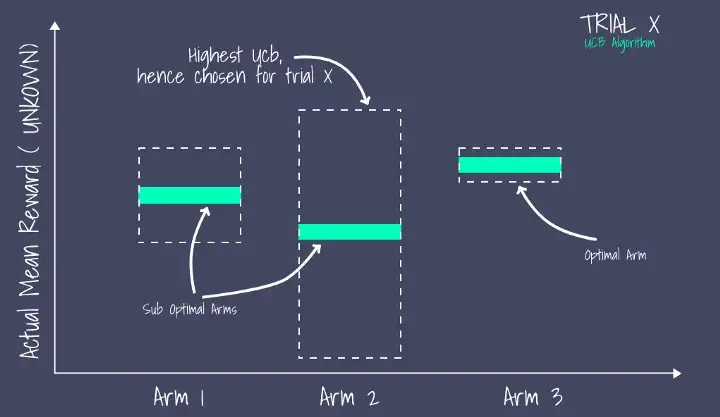
\includegraphics[scale=0.58]{Images/Learning_compensations/linucb.jpg}
    \caption[LinUCB algorithm for choosing the best arm.]{LinUCB algorithm for choosing the best arm \cite{recommender2020}.}
    \label{fig:linucb}
\end{figure}

We implemented the LinUCB algorithm from \ref{alg:linucb} \cite{recommender2020}. Let $d$ be the number of variables of the context $x_{t,a}$ (state). In our experiments, $d=3$. $A_a$ and $b_a$ are the variables used in ridge regression. This regression tries to find the correlation between state and reward. Lines 2-5 initialize both $A_a$ and $b_a$ for all actions in the set of possible actions $A_t$. This initialization makes all arms (actions) start with a very high UCB, forcing each arm to be chosen at least once. So, it calculates the UCB for every arm at each step $t$ (lines 6-10). To do so, line 8 calculates the ridge regression ($\hat{\theta_a}$), and line 9 applies it to find the UCB. The UCB $\rho_{t, a}$ is calculated by $\rho_{t, a} \leftarrow \hat{\theta_a}^\top x_{t,a} + \nu \sqrt{x_{t,a}^\top A_{a}^{-1} x_{t,a}}$ where the first part ($\hat{\theta_a}^\top x_{t,a}$) is the expected mean, and the second part ($\nu \sqrt{x_{t,a}^\top A_{a}^{-1} x_{t,a}}$) is the upper confidence bound. $\nu$ is a hyperparameter to indicate the importance of the standard deviation in the UCB. The higher $\nu$ is, the wider the confidence bounds become. So, a higher $\nu$ results in a higher emphasis on exploration instead of exploitation. We defined $\nu = 20$ after some experiments, with the best results with this value.

\IncMargin{1em}
\begin{algorithm}[!htb]
    \footnotesize
    \SetAlgoLined
    \Begin{
        \ForAll{a $\in A_t$ }{
            $A_a \leftarrow I_d$ (d-dimensional identity matrix)\;
            $b_a \leftarrow 0_{dx1}$ (d-dimensional zero vector)\;
        }        
        \For{t = 0, 1, 2, 3, ..., T}{
            \ForAll{a $\in A_t$ }{
                $\hat{\theta_a} \leftarrow A_{a}^{-1}b_a$\;
                $\rho_{t, a} \leftarrow \hat{\theta_a}^\top x_{t,a} + \nu \sqrt{x_{t,a}^\top A_{a}^{-1} x_{t,a}}$\;
            }
            Choose arm $a_t = \arg\max_{a \in A_t} \rho_{t, a}$, and observe a real-valued reward $r_t$\; 
            $A_{a_{t}} \leftarrow A_{a_{t}} + x_{t,a_{t}} x_{t,a_{t}}^\top$\;
            $b_{a_{t}} \leftarrow b_{a_{t}} + r_t x_{t,a_{t}}$\;
        }
    }
    \caption{LinUCB algorithm \cite{li2010contextual}.}
    \label{alg:linucb}
\end{algorithm}
\DecMargin{1em}

After that, line 11 verifies the action $a_t$ with higher UCB among the actions in $A_t$. This line applies the action and receives a reward $r_t$. Then, it updates the ridge regression variables ($A_a$ and $b_a$) for action $a_t$ in lines 12 and 13 ($A_{a_{t}}$ and $b_{a_{t}}$). Differently from Q-Learning, Contextual Multi-Armed Bandit does not need a discretization of the state. Therefore, we can use the state directly without modifications.

\section{Results Evaluation}

After presenting the algorithms, we apply them to the critical scenarios from the previous chapter. We have four different RL executions combining the RL algorithm and action types: 

\begin{enumerate}
    \item \emph{Bandit + heuristic};
    \item \emph{Q-Learning + heuristic};
    \item \emph{Bandit + hour};
    \item \emph{Q-Learning + hour};
\end{enumerate}

These algorithms use the same scheduling from Chapter \ref{cha:power_compensations}, changing only in which step compensating. We run 200 iterations for each critical case of each RL algorithm with the different reward types. The idea is to verify if the RL algorithms can learn by repeating the same inputs (workload and weather). In addition, we want to verify if they can improve the number of finished jobs. We do not execute the random cases due to their complexity. There are 100 different cases, demanding high processing time for executing 200 iterations of each one. Again, the critical cases are:
\begin{enumerate}
    \item \emph{Critical 1}: Profile best-case and workload in the beginning;
    \item \emph{Critical 2}: Profile best-case and workload in the end;
    \item \emph{Critical 3}: Profile worst-case and workload in the beginning;
    \item \emph{Critical 4}: Profile worst-case and workload in the end;
\end{enumerate}

The results from the baselines and compensation policies (\emph{Last}, \emph{Next}, \emph{Peak}, and \emph{Workload}) are the same results from the previous chapter. We compare them with the new results from Reinforcement Learning. The results of the random algorithms are an average of 200 iterations.

\subsection{Started Jobs Reward}

Beginning with the Started Jobs reward, we present the results in the four critical cases in Figures \ref{fig:started_reward_results_critical_1}, \ref{fig:started_reward_results_critical_2}, \ref{fig:started_reward_results_critical_3}, and \ref{fig:started_reward_results_critical_4}. Each figure shows five graphs. The first two on top are the graphs about the finished jobs. The two graphs in the middle are the battery level and wasted energy. The last graph is the reward evolution over the 200 iterations. The reward is calculated by summing all rewards from the different actions inside the iteration.

\begin{figure}[!htb]
    \centering
    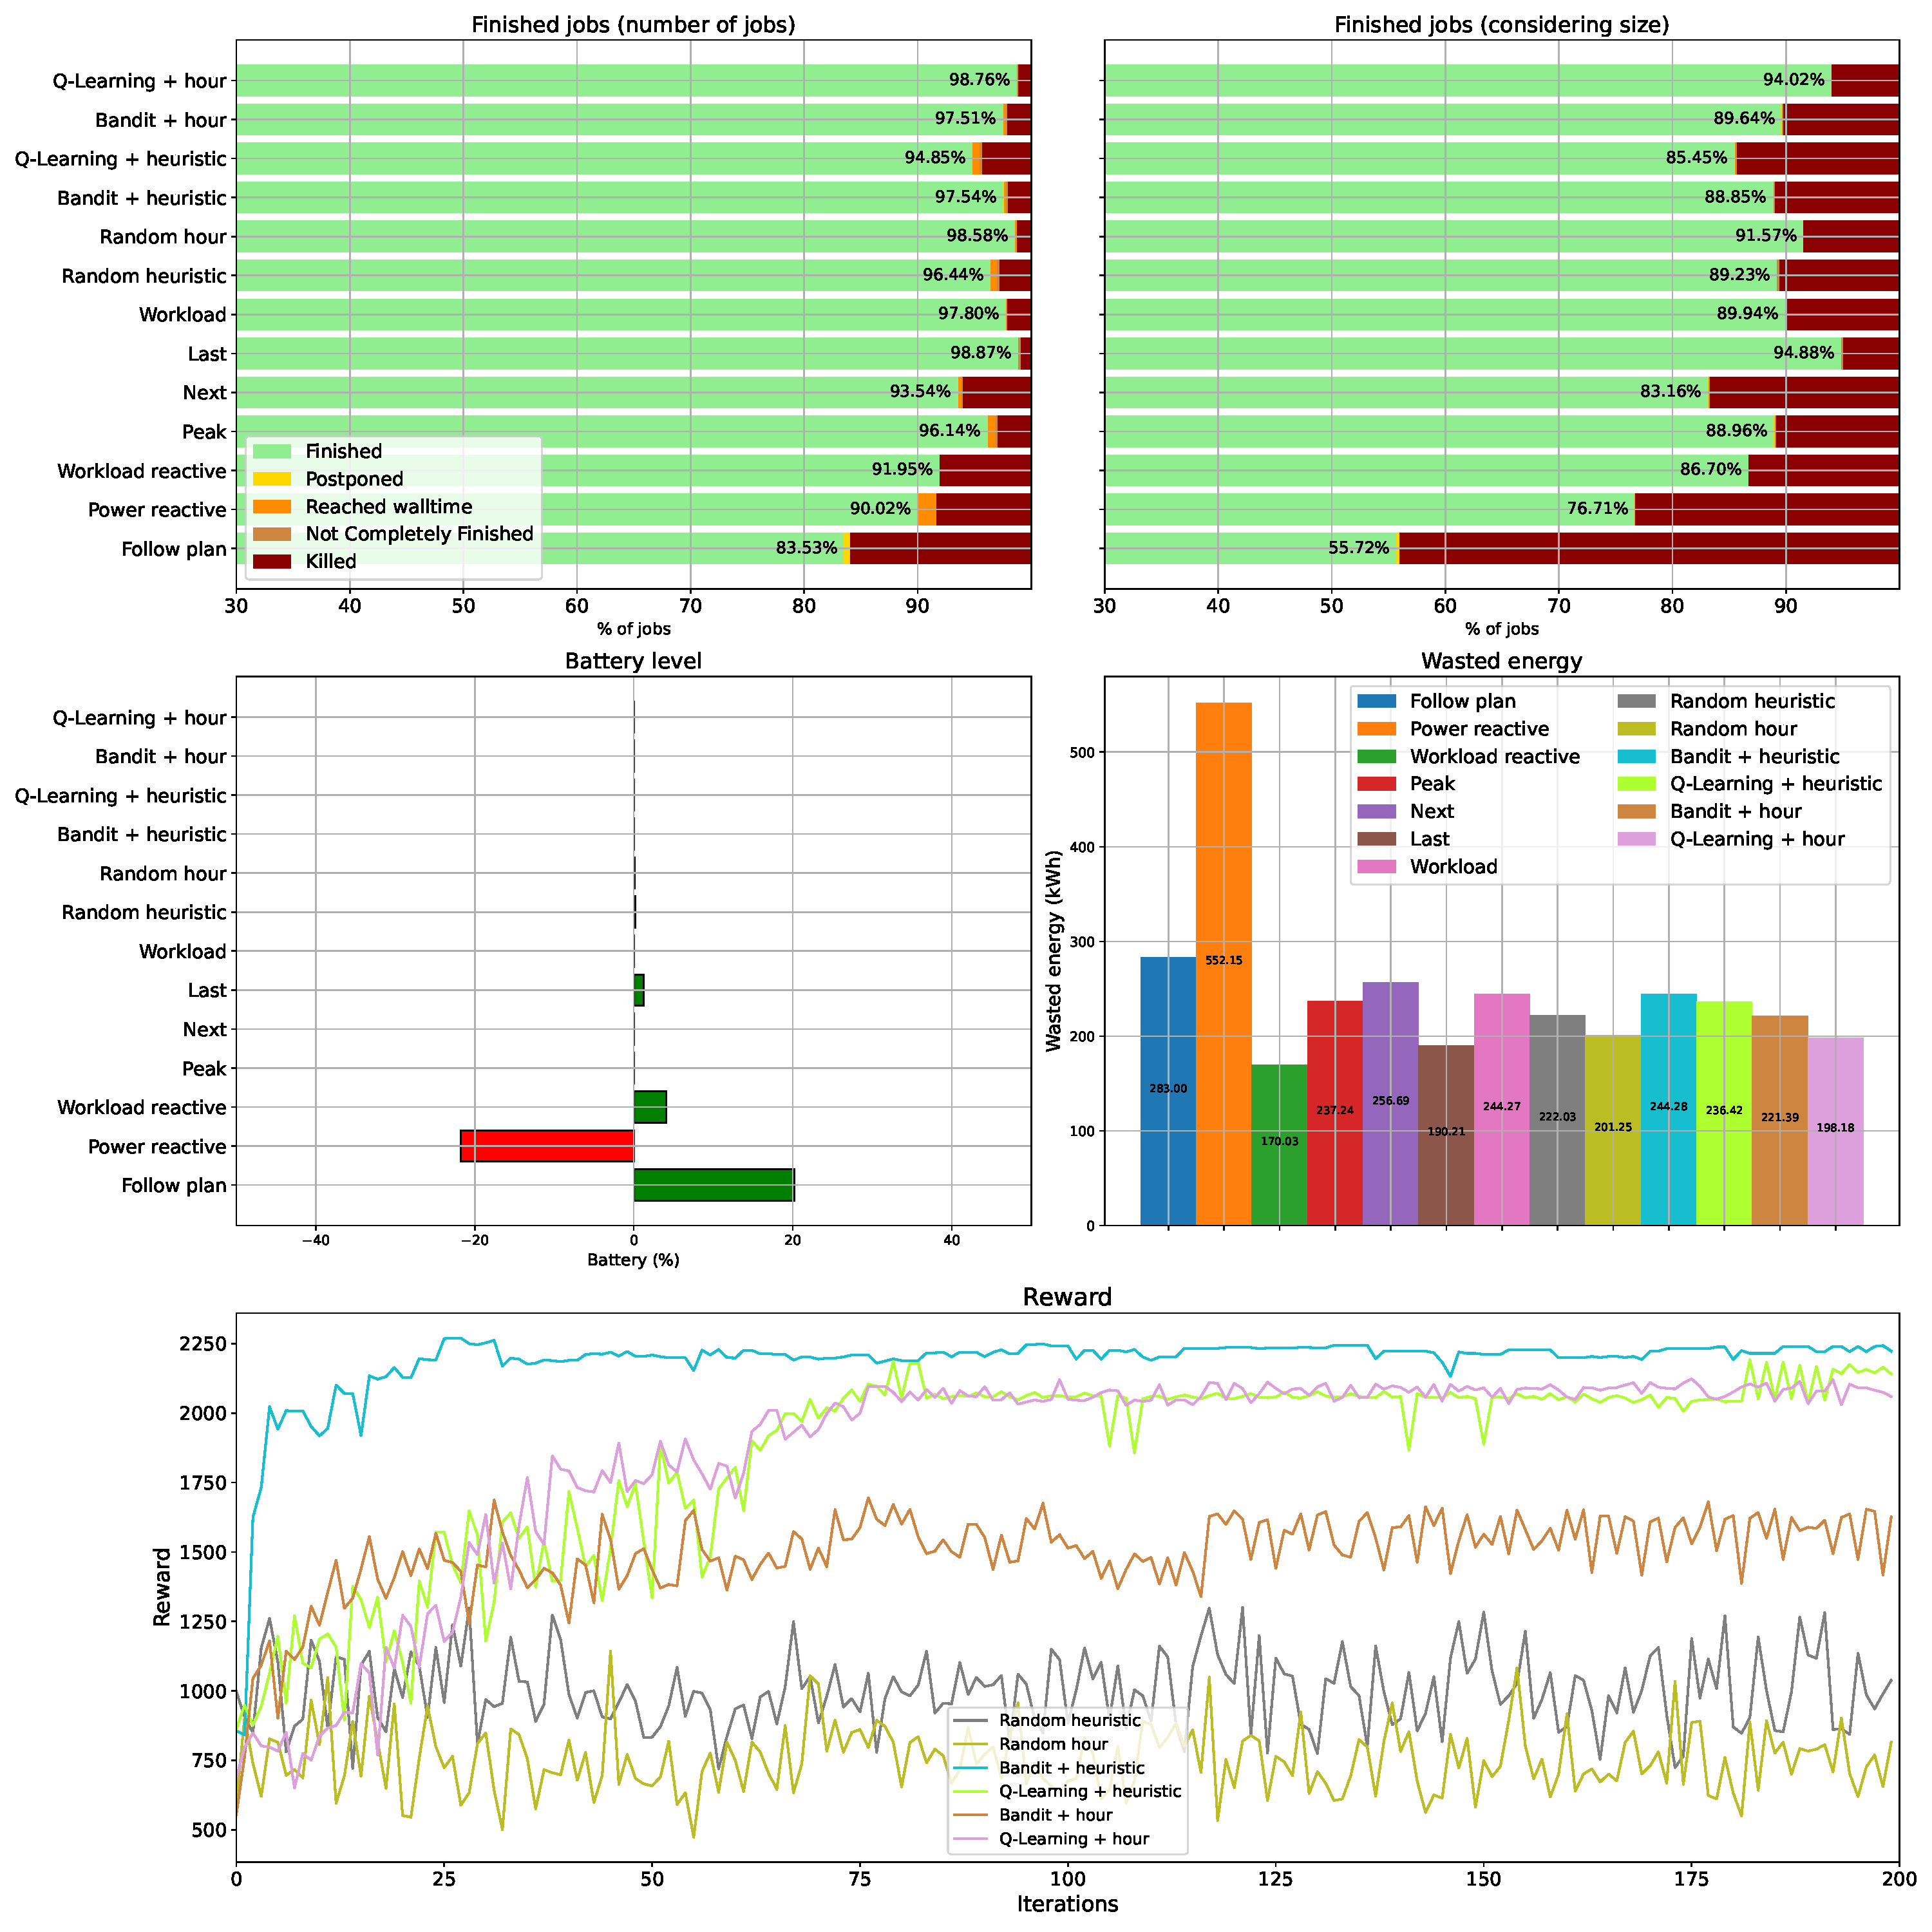
\includegraphics[scale=0.29]{Images/Learning_compensations/reward_started_profile_best_workload_1_with_noise_state_delta.pdf}
    \caption{Results of reward started jobs in critical case 1.}
    \label{fig:started_reward_results_critical_1}
\end{figure}

\begin{figure}[!htb]
    \centering
    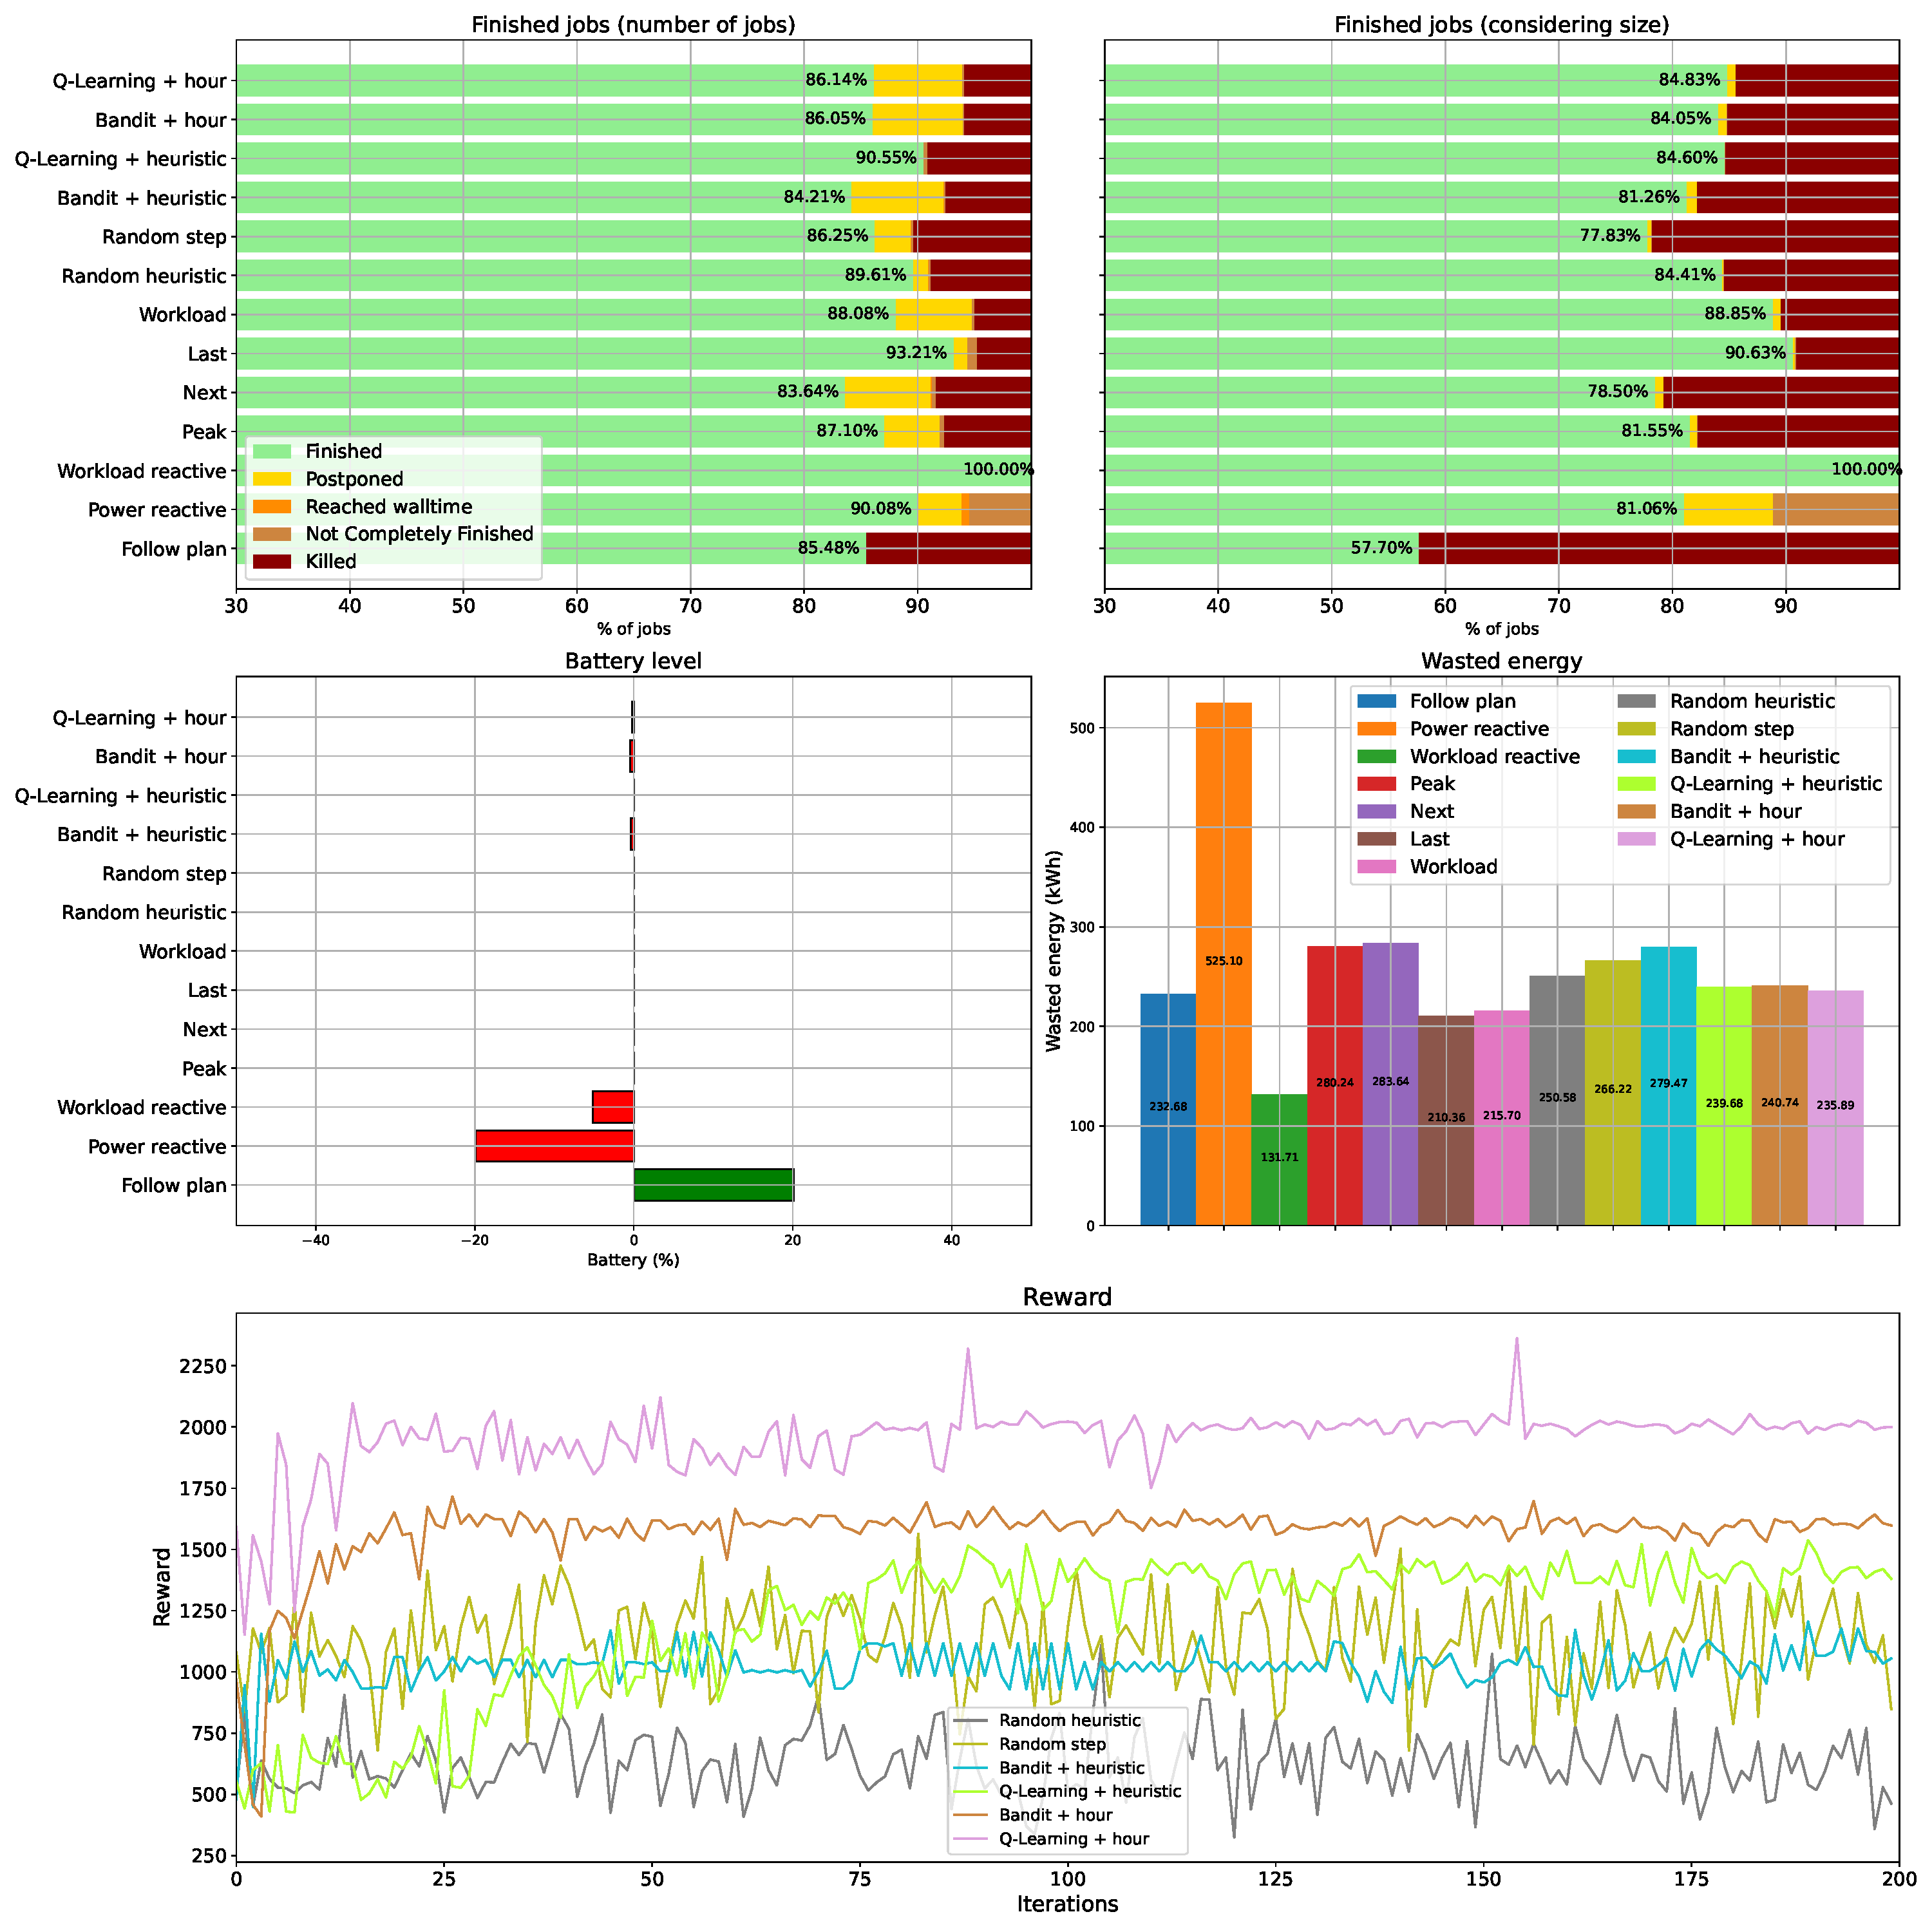
\includegraphics[scale=0.29]{Images/Learning_compensations/reward_started_profile_best_workload_2_with_noise_state_delta.pdf}
    \caption{Results of reward started jobs in critical case 2.}
    \label{fig:started_reward_results_critical_2}
\end{figure}

\begin{figure}[!htb]
    \centering
    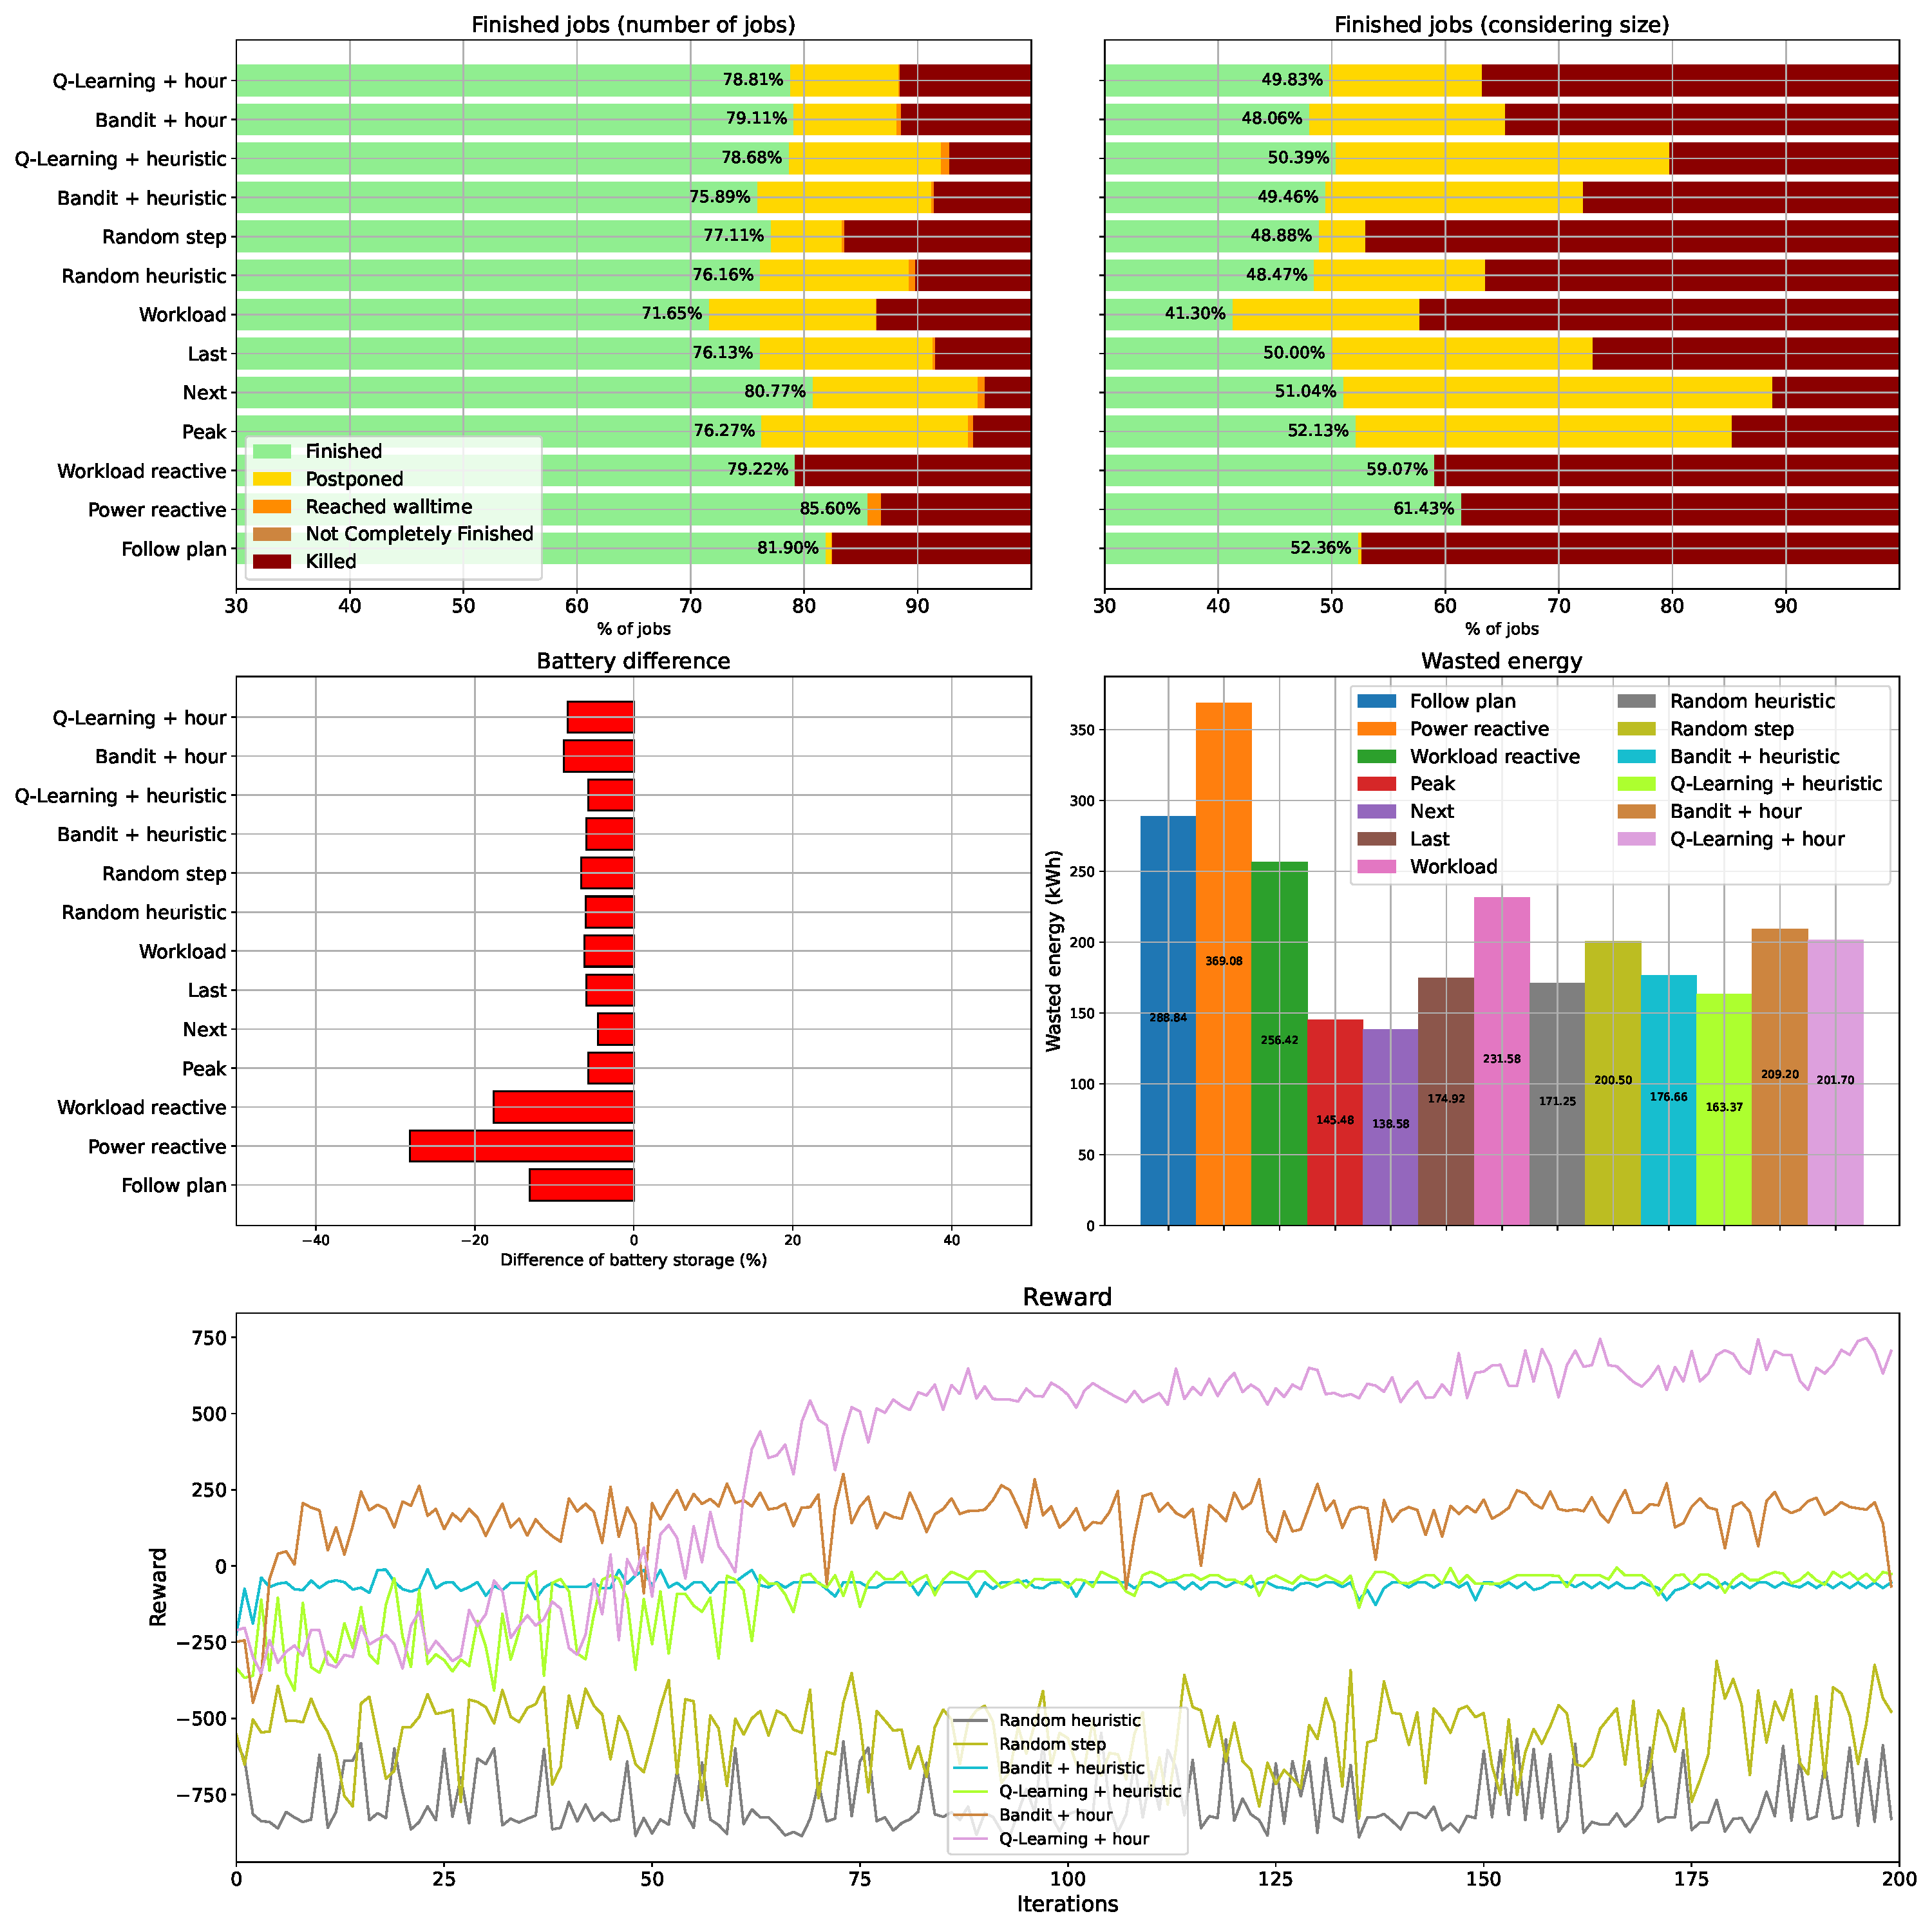
\includegraphics[scale=0.29]{Images/Learning_compensations/reward_started_profile_worst_workload_1_with_noise_state_delta.pdf}
    \caption{Results of reward started jobs in critical case 3.}
    \label{fig:started_reward_results_critical_3}
\end{figure}

\begin{figure}[!htb]
    \centering
    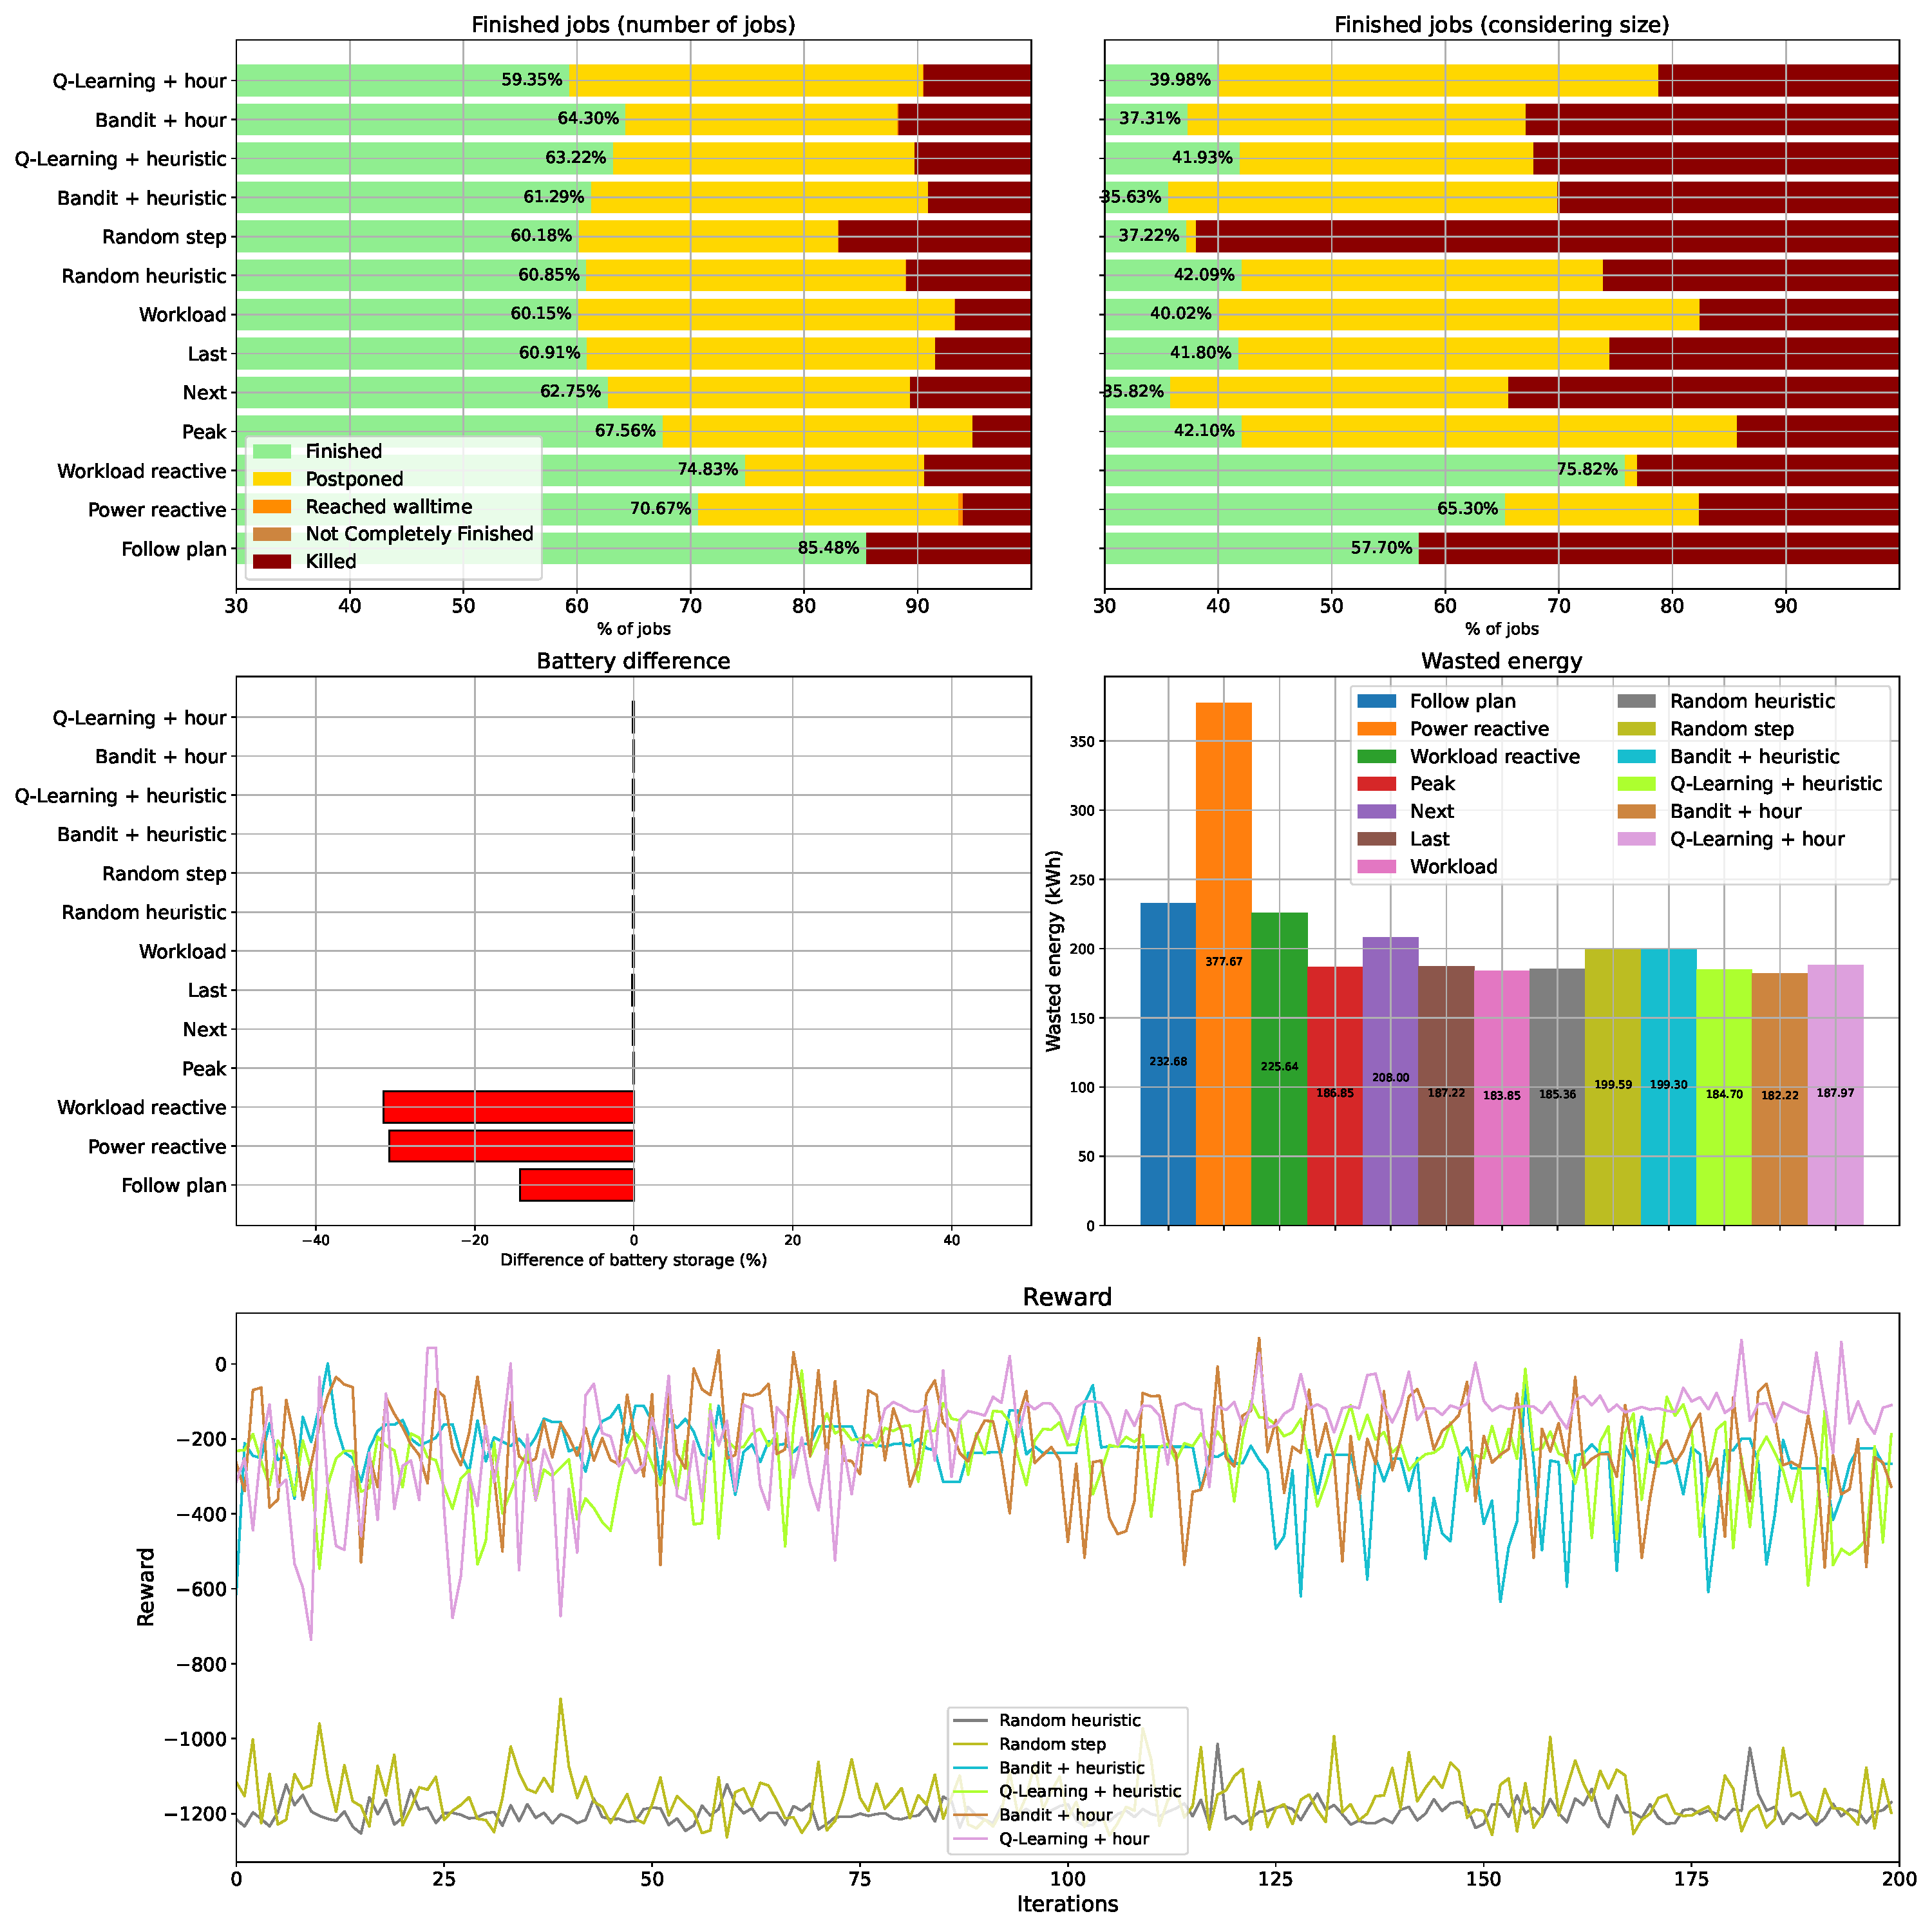
\includegraphics[scale=0.29]{Images/Learning_compensations/reward_started_profile_worst_workload_2_with_noise_state_delta.pdf}
    \caption{Results of reward started jobs in critical case 4.}
    \label{fig:started_reward_results_critical_4}
\end{figure}

Figure \ref{fig:started_reward_results_critical_1} shows that in critical case 1, all RL improved their reward over time. They started with similar rewards to random executions. However, at the end of 200 iterations, they improved the reward. This result shows that the algorithms find the decisions which give higher rewards. Considering the reward, the best algorithm is \emph{Bandit + heuristic}. \emph{Q-Learning + heuristic}, \emph{Q-Learning + hour}, and \emph{Bandit + hour} have very similar rewards, with \emph{Bandit + hour} having more variance than the other two. However, considering the finished jobs in number (first graph), the results indicate \emph{Q-Learning + hour} as the best one, with \emph{Bandit + hour} as the second one with a similar result. So, even if \emph{Bandit + heuristic} has the best reward, it does not mean it has the best global QoS. This result shows a problem in this reward, where just starting jobs does not guarantee they will finish. Additionally, the best RL result is still worst than the \emph{Last} policy in the finished jobs metric (both in number and size). \emph{Random step} has a similar result to the best RL algorithm, showing that even a random choice is a good option here. Considering the Battery level, all RL algorithms have the same results. Finally, both Bandit and Q-Learning algorithms expend more energy than \emph{Last} policy in this case.

The results of critical case 2 in Figure \ref{fig:started_reward_results_critical_2} show that both RL algorithms using the action of the hour have the highest reward. However, it is not translated to good QoS. These algorithms have worse Finished jobs in number than \emph{Q-Learning + heuristic}, \emph{Random step}, \emph{Random heuristic}, \emph{Workload}, \emph{Last}, and \emph{Peak} policies (ignoring the baselines). \emph{Q-Learning + heuristic} has the best number of finished jobs among the RL algorithms, with the third-best reward. However, it kills more jobs. \emph{Bandit + Heuristic} has the worst QoS among the RL algorithms. Both random algorithms finished several jobs, but they also have a high number of killed jobs. Considering the size, \emph{Q-Learning + hour} and \emph{Q-Learning + heuristic} finished more jobs than the other RL algorithms and the random, but they are still far from \emph{Workload} and \emph{Last} policies. Regarding the battery level, all RL algorithms ended close to the target level. Finally, \emph{Q-Learning + heuristic}, \emph{Bandit + hour}, and \emph{Q-Learning + hour} wasted less energy than the random algorithms but more than \emph{Last} and \emph{Workload} policies.

Starting the cases with less energy, Figure \ref{fig:started_reward_results_critical_3} illustrates the results of critical case 3. Here, again, all RL algorithms have higher rewards than both random algorithms. Again, the \emph{Q-Learning + hour} and \emph{Bandit + hour} have the best results among the RL algorithms. \emph{Bandit + hour} has a lower reward but a higher number of jobs finished. However, all RL algorithms have fewer finished jobs than \emph{Next} policy (in number and size). Besides, they kill more jobs than \emph{Next} and \emph{Peak} policies. These results show again that the RL could not learn which are the best policies to use. Considering the battery level, \emph{Q-Learning + hour} and \emph{Bandit + hour} use slightly more battery than the other policies. Nevertheless, they are all below the baselines. Finally, the wasted energy results of the RL algorithms are higher than the \emph{Peak} and \emph{Next} policies.

Figure \ref{fig:started_reward_results_critical_4} presents the last scenario, critical case 4. All RL algorithms have higher rewards than random heuristics. In this scenario, the reward varies a lot, showing that it still has indecision to define the best actions. \emph{Bandit + hour} has the highest number of finished jobs among the RL algorithms. However, it kills more than the other RL algorithms. No RL algorithm is better than the \emph{Peak} policy in finished and killed jobs in both number and size (ignoring the baselines). All RL algorithms finished with the battery level close to the target. Finally, only \emph{Bandit + hour} wasted less energy than \emph{Workload} (the best policy).

Consolidating the results of the Started Jobs Reward, Table \ref{tab:ranking_started} presents a ranking of the different tested scenarios. We highlight in green the top 3 results on each metric for each scenario. The bottom 3 results are in red. Both finished and killed jobs are considered in number. Killed jobs are: killed jobs + reach the walltime + not completely finished. For SoC, we assume the best results as the higher real SoC at the end of the time window. The learning algorithms could not improve the metrics, compared to the reactive algorithms and the policies from Chapter \ref{cha:power_compensations}. In the two scenarios with profile best-case, \emph{Last} has the best results, with no metric at bottom 3 and 7 metrics at top 3. On the other hand, in profile worst-case executions, \emph{Next} and \emph{Peak} are quite good. The RL algorithms have some results in top 3, but they generally stay out of the top 3 results. Regarding the reward, it is possible to notice that \emph{Q-Learning + hour} and \emph{Bandit + hour} improved the reward after 200 iterations. Usually, the reward from these cases has a distance from the random rewards after 200 iterations. This result indicates that the RL learning algorithms are learning the policies to choose the actions which give a high reward. However, having a high reward does not result in good global results (mainly finished/killed jobs). This reward reinforces the actions which put more energy into steps that start more jobs. However, starting jobs does not mean that they will finish. So, it can start several jobs but kill a lot also. Aiming to solve this problem (starting some jobs but not finishing them), we proposed the next reward.

% Please add the following required packages to your document preamble:
% \usepackage{multirow}

\begin{landscape}

\mbox{}\vfill

\begin{table*}[htp]
    \centering
    \caption{Consolidate average results in every scenario for reward started.}
    \label{tab:ranking_started}
    \scriptsize
    \begin{tabular}{c|l||l|l|l|l|l|l|l|l|l|l|l|l|l}
    \hline
    Scenario & Metric & \begin{tabular}[c]{@{}l@{}}Follow\\ plan\end{tabular} & \begin{tabular}[c]{@{}l@{}}Power\\ reactive\end{tabular} & \begin{tabular}[c]{@{}l@{}}Workload\\ reactive\end{tabular} & Peak & Next & Last & Load & \begin{tabular}[c]{@{}l@{}}Rand.\\ heuris.\end{tabular} & \begin{tabular}[c]{@{}l@{}}Rand.\\ step\end{tabular} & \begin{tabular}[c]{@{}l@{}}Bandit +\\ heuristic\end{tabular} & \begin{tabular}[c]{@{}l@{}}Q-Learn. +\\ heuristic\end{tabular} & \begin{tabular}[c]{@{}l@{}}Bandit +\\ hour\end{tabular} & \begin{tabular}[c]{@{}l@{}}Q-Learn. +\\ hour\end{tabular} \\ \hline \hline
    \multirow{4}{*}{\begin{tabular}[c]{@{}c@{}}Profile best-case \\ and\\ workload in \\ beginning\end{tabular}} & Finished jobs & {\cellcolor{red!75}}\nth{13} & {\cellcolor{red!50}}\nth{12} & {\cellcolor{red!25}}\nth{11} & \nth{7} & \nth{10} & {\cellcolor{green!75}}\nth{1} & \nth{5} & \nth{6} & {\cellcolor{green!25}}\nth{3} & \nth{8} & \nth{9} & \nth{4} & {\cellcolor{green!50}}\nth{2} \\ \cline{2-15} 
     & Killed jobs & {\cellcolor{red!75}}\nth{13} & {\cellcolor{red!50}}\nth{12} & {\cellcolor{red!25}}\nth{11} & \nth{7} & \nth{10} & {\cellcolor{green!75}}\nth{1} & \nth{5} & \nth{6} & {\cellcolor{green!25}}\nth{3} & \nth{8} & \nth{9} & \nth{4} & {\cellcolor{green!50}}\nth{2} \\ \cline{2-15} 
     & SoC & {\cellcolor{green!75}}\nth{1} & {\cellcolor{red!75}}\nth{13} & {\cellcolor{green!50}}\nth{2} & \nth{9} & {\cellcolor{red!50}}\nth{12} & {\cellcolor{green!25}}\nth{3} & \nth{7} & \nth{4} & \nth{5} & {\cellcolor{red!25}}\nth{11} & \nth{8} & \nth{10} & \nth{6} \\ \cline{2-15} 
     & Wasted energy & {\cellcolor{red!25}}\nth{11} & {\cellcolor{red!75}}\nth{13} & {\cellcolor{green!75}}\nth{1} & \nth{7} & \nth{10} & {\cellcolor{green!50}}\nth{2} & \nth{8} & \nth{6} & \nth{4} & {\cellcolor{red!50}}\nth{12} & \nth{9} & \nth{5} & {\cellcolor{green!25}}\nth{3} \\ \hline
    \multirow{4}{*}{\begin{tabular}[c]{@{}c@{}}Profile best-case \\ and\\ workload in end\end{tabular}} & Finished jobs & {\cellcolor{red!25}}\nth{11} & \nth{4} & {\cellcolor{green!75}}\nth{1} & \nth{7} & {\cellcolor{red!75}}\nth{13} & {\cellcolor{green!50}}\nth{2} & \nth{6} & \nth{5} & \nth{8} & {\cellcolor{red!50}}\nth{12} & {\cellcolor{green!25}}\nth{3} & \nth{10} & \nth{9} \\ \cline{2-15} 
     & Killed jobs & {\cellcolor{red!75}}\nth{13} & \nth{6} & {\cellcolor{green!75}}\nth{1} & \nth{8} & \nth{9} & {\cellcolor{green!25}}\nth{3} & {\cellcolor{green!50}}\nth{2} & \nth{10} & {\cellcolor{red!50}}\nth{12} & \nth{7} & {\cellcolor{red!25}}\nth{11} & \nth{4} & \nth{5} \\ \cline{2-15} 
     & SoC & {\cellcolor{green!75}}\nth{1} & {\cellcolor{red!75}}\nth{13} & {\cellcolor{red!50}}\nth{12} & \nth{4} & \nth{5} & \nth{6} & \nth{7} & {\cellcolor{green!25}}\nth{3} & \nth{8} & \nth{10} & {\cellcolor{green!50}}\nth{2} & {\cellcolor{red!25}}\nth{11} & \nth{9} \\ \cline{2-15} 
     & Wasted energy & \nth{4} & {\cellcolor{red!75}}\nth{13} & {\cellcolor{green!75}}\nth{1} & {\cellcolor{red!25}}\nth{11} & {\cellcolor{red!50}}\nth{12} & {\cellcolor{green!50}}\nth{2} & {\cellcolor{green!25}}\nth{3} & \nth{8} & \nth{9} & \nth{10} & \nth{6} & \nth{7} & \nth{5} \\ \hline
    \multirow{4}{*}{\begin{tabular}[c]{@{}c@{}}Profile worst-case \\ and\\ workload in \\ beginning\end{tabular}} & Finished jobs & {\cellcolor{green!50}}\nth{2} & {\cellcolor{green!75}}\nth{1} & \nth{4} & \nth{9} & {\cellcolor{green!25}}\nth{3} & {\cellcolor{red!25}}\nth{11} & {\cellcolor{red!75}}\nth{13} & \nth{10} & \nth{8} & {\cellcolor{red!50}}\nth{12} & \nth{7} & \nth{5} & \nth{6} \\ \cline{2-15} 
     & Killed jobs & {\cellcolor{red!50}}\nth{12} & \nth{10} & {\cellcolor{red!75}}\nth{13} & {\cellcolor{green!50}}\nth{2} & {\cellcolor{green!75}}\nth{1} & \nth{4} & \nth{9} & \nth{6} & {\cellcolor{red!25}}\nth{11} & \nth{5} & {\cellcolor{green!25}}\nth{3} & \nth{8} & \nth{7} \\ \cline{2-15} 
     & SoC & {\cellcolor{red!25}}\nth{11} & {\cellcolor{red!75}}\nth{13} & {\cellcolor{red!50}}\nth{12} & {\cellcolor{green!25}}\nth{3} & {\cellcolor{green!75}}\nth{1} & \nth{4} & \nth{7} & \nth{6} & \nth{8} & \nth{5} & {\cellcolor{green!50}}\nth{2} & \nth{10} & \nth{9} \\ \cline{2-15} 
     & Wasted energy & {\cellcolor{red!50}}\nth{12} & {\cellcolor{red!75}}\nth{13} & {\cellcolor{red!25}}\nth{11} & {\cellcolor{green!50}}\nth{2} & {\cellcolor{green!75}}\nth{1} & \nth{5} & \nth{10} & \nth{4} & \nth{7} & \nth{6} & {\cellcolor{green!25}}\nth{3} & \nth{9} & \nth{8} \\ \hline
    \multirow{4}{*}{\begin{tabular}[c]{@{}c@{}}Profile worst-case \\ and\\ workload in end\end{tabular}} & Finished jobs & {\cellcolor{green!75}}\nth{1} & {\cellcolor{green!25}}\nth{3} & {\cellcolor{green!50}}\nth{2} & \nth{4} & \nth{7} & \nth{9} & {\cellcolor{red!50}}\nth{12} & \nth{10} & {\cellcolor{red!25}}\nth{11} & \nth{8} & \nth{6} & \nth{5} & {\cellcolor{red!75}}\nth{13} \\ \cline{2-15} 
     & Killed jobs & {\cellcolor{red!50}}\nth{12} & {\cellcolor{green!50}}\nth{2} & \nth{6} & {\cellcolor{green!75}}\nth{1} & \nth{9} & \nth{4} & {\cellcolor{green!25}}\nth{3} & \nth{10} & {\cellcolor{red!75}}\nth{13} & \nth{5} & \nth{8} & {\cellcolor{red!25}}\nth{11} & \nth{7} \\ \cline{2-15} 
     & SoC & {\cellcolor{red!25}}\nth{11} & {\cellcolor{red!50}}\nth{12} & {\cellcolor{red!75}}\nth{13} & {\cellcolor{green!75}}\nth{1} & {\cellcolor{green!25}}\nth{3} & \nth{10} & \nth{4} & \nth{9} & \nth{8} & \nth{6} & \nth{5} & {\cellcolor{green!50}}\nth{2} & \nth{7} \\ \cline{2-15} 
     & Wasted energy & {\cellcolor{red!50}}\nth{12} & {\cellcolor{red!75}}\nth{13} & {\cellcolor{red!25}}\nth{11} & \nth{5} & \nth{10} & \nth{6} & {\cellcolor{green!50}}\nth{2} & \nth{4} & \nth{9} & \nth{8} & {\cellcolor{green!25}}\nth{3} & {\cellcolor{green!75}}\nth{1} & \nth{7} \\ \hline
    \end{tabular}
\end{table*}
\vfill
\end{landscape}

\clearpage

\subsection{Finished Jobs Reward}

The next reward aims to solve the problem of starting jobs and not finishing them. So, this reward reinforces the actions that help to finish more jobs. Figures \ref{fig:touched_reward_results_critical_1}, \ref{fig:touched_reward_results_critical_2}, \ref{fig:touched_reward_results_critical_3}, and \ref{fig:touched_reward_results_critical_4} present the results of this reward. 

\begin{figure}[!htb]
    \centering
    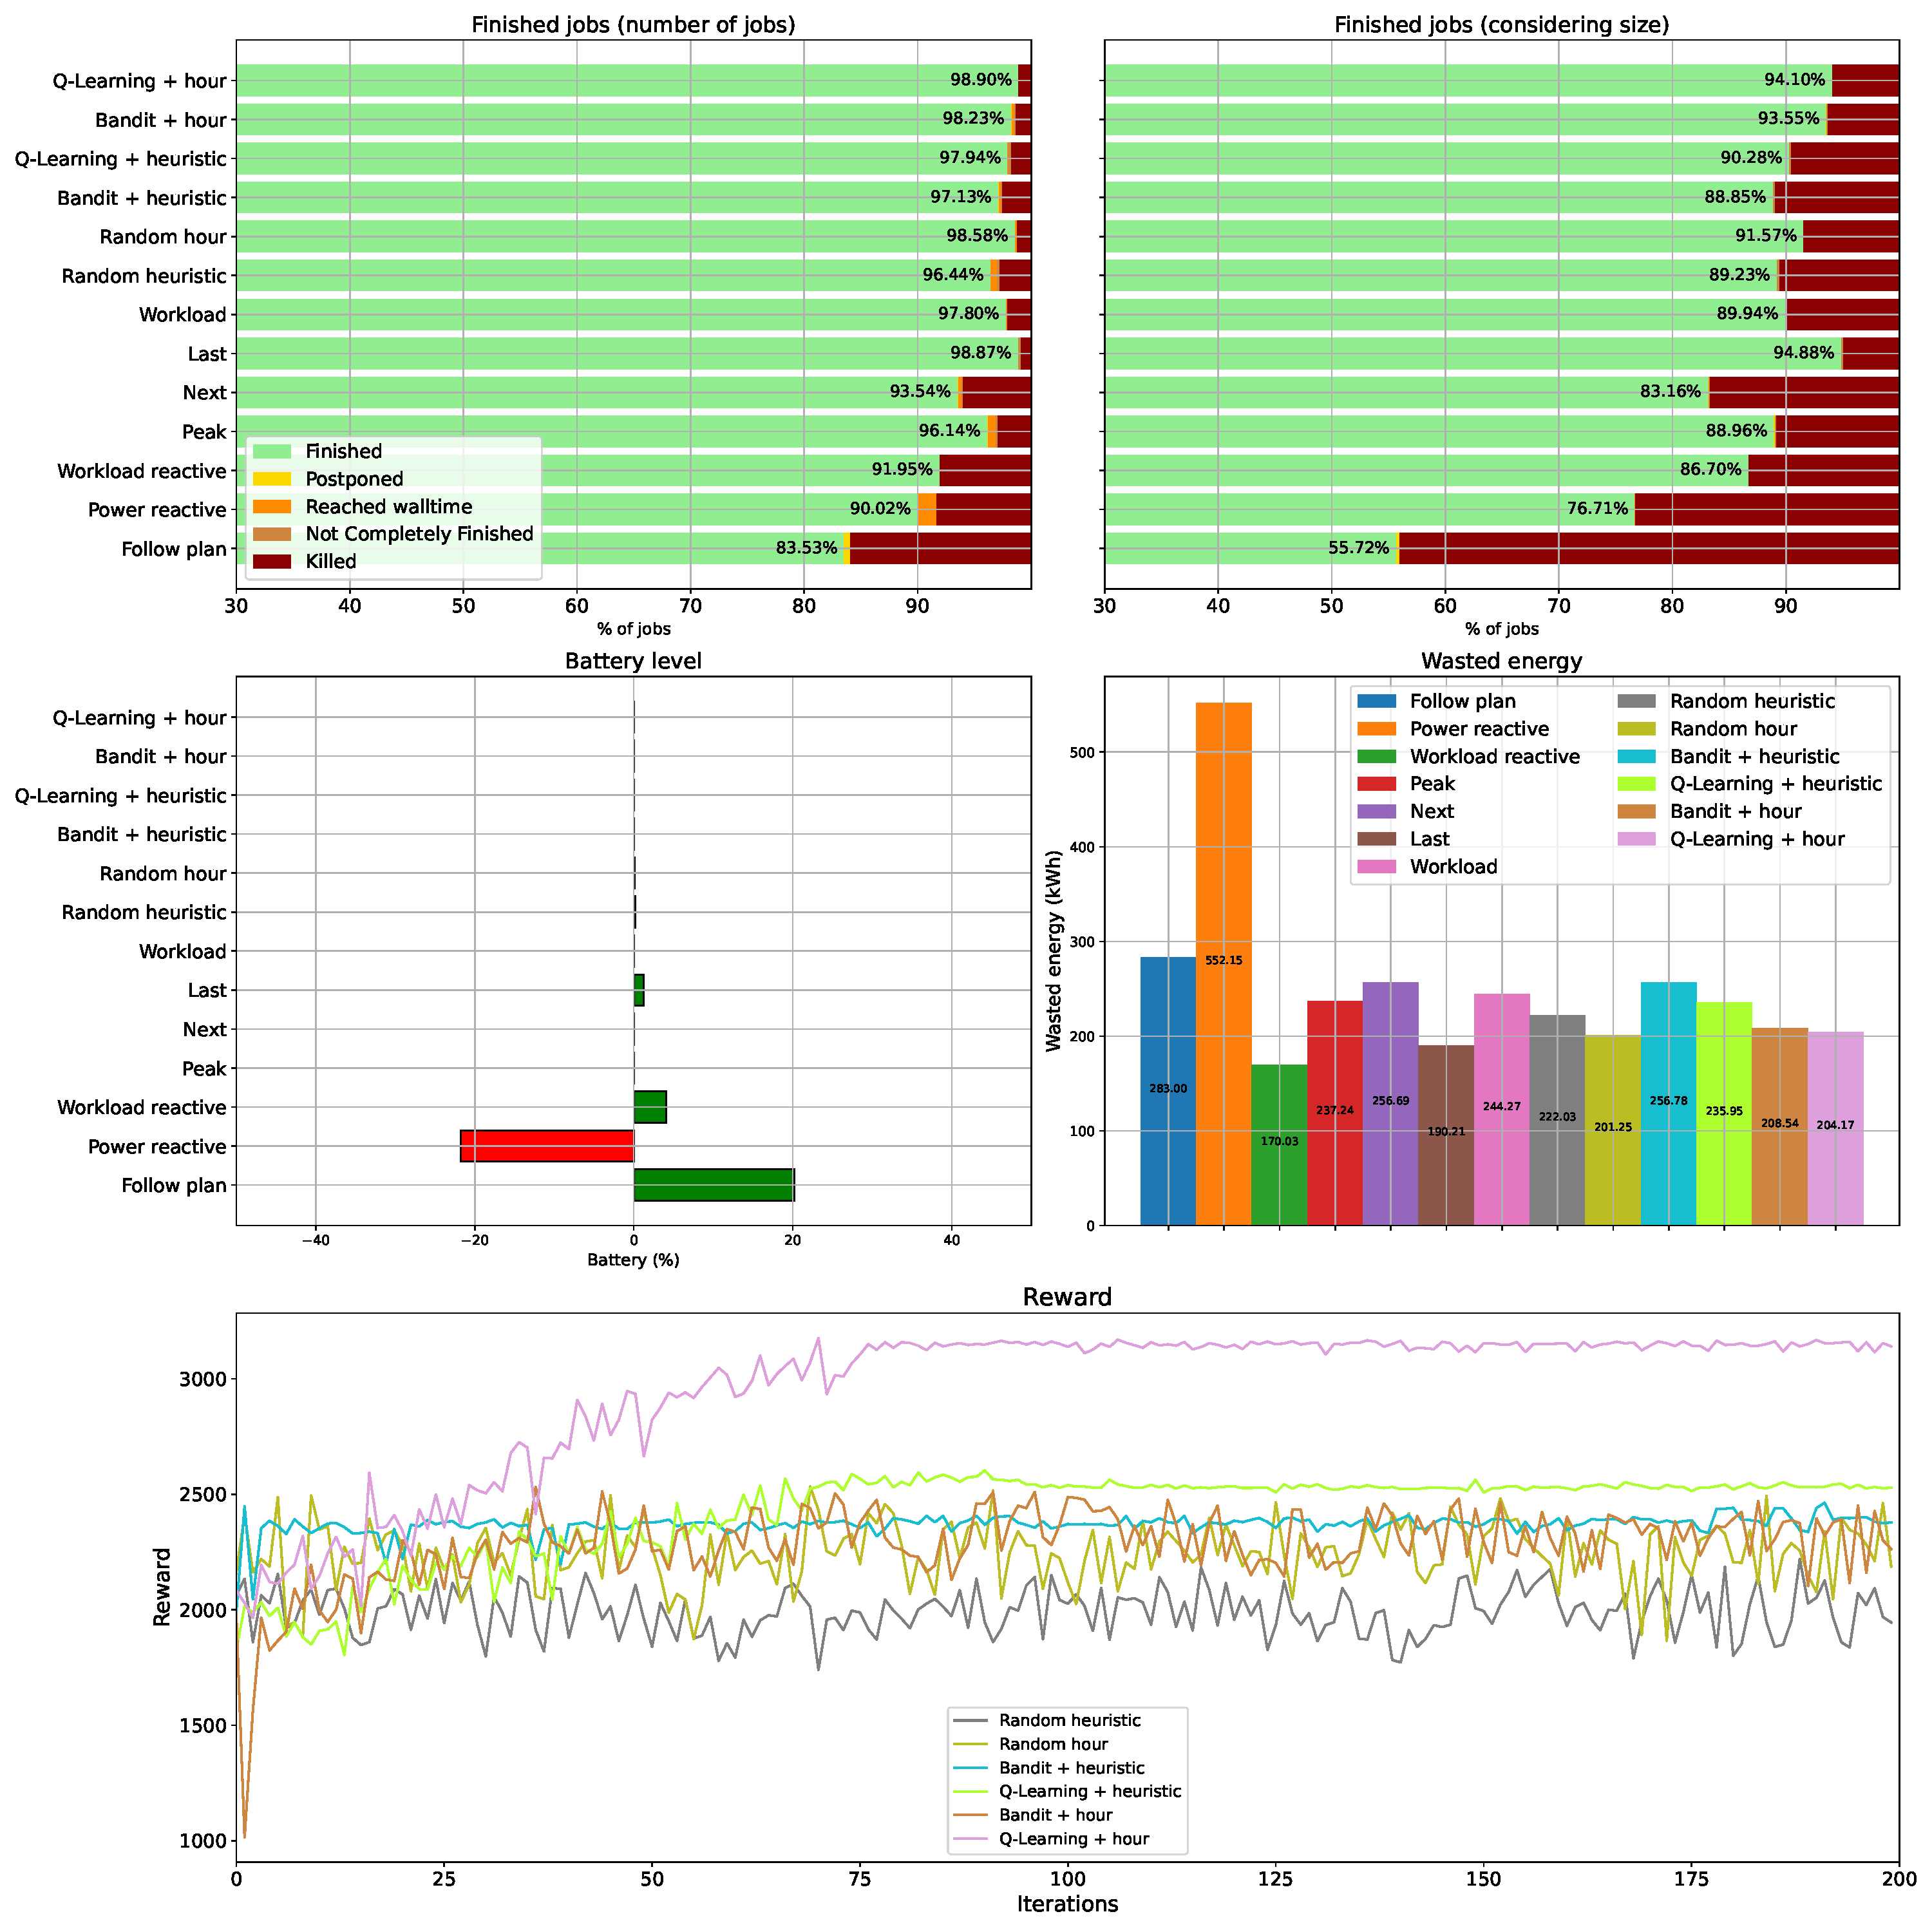
\includegraphics[scale=0.29]{Images/Learning_compensations/reward_finished_touched_profile_best_workload_1_with_noise_state_delta.pdf}
    \caption{Results of finished jobs reward in critical case 1.}
    \label{fig:touched_reward_results_critical_1}
\end{figure}

We introduce in this section a new graph in Figures \ref{fig:reward_from_jobs_critical_1}, \ref{fig:reward_from_jobs_critical_2}, \ref{fig:reward_from_jobs_critical_3}, and \ref{fig:reward_from_jobs_critical_4}. In these figures, the graphs on the top are from finished jobs, where blue+red means the total number of finished jobs, blue is the finished jobs included in the reward, and red is the finished jobs ignored in the reward. The higher the red+blue, the better. On the other hand, the bottom graphs are the killed jobs, where blue+red means the total number of killed jobs, blue is the jobs included in the reward, and red is the jobs finished but ignored by the reward. The higher the red+blue, the worse. The idea in these graphs is to see if, over the iterations (x-axis), the global finished jobs increase and the killed jobs reduce. Besides, these graphs illustrate if the reward reflects our objective of improving the global QoS (by improving locally). A job is considered ignored in the reward when no previous step impacts the power usage of the steps where it executes. For example, let's say a job executes from steps 50 to 52. A job is ignored in the reward if no previous step increases the power usage in steps 50, 51, and 52. The same for killed jobs.

\begin{figure}[!htb]
    \centering
    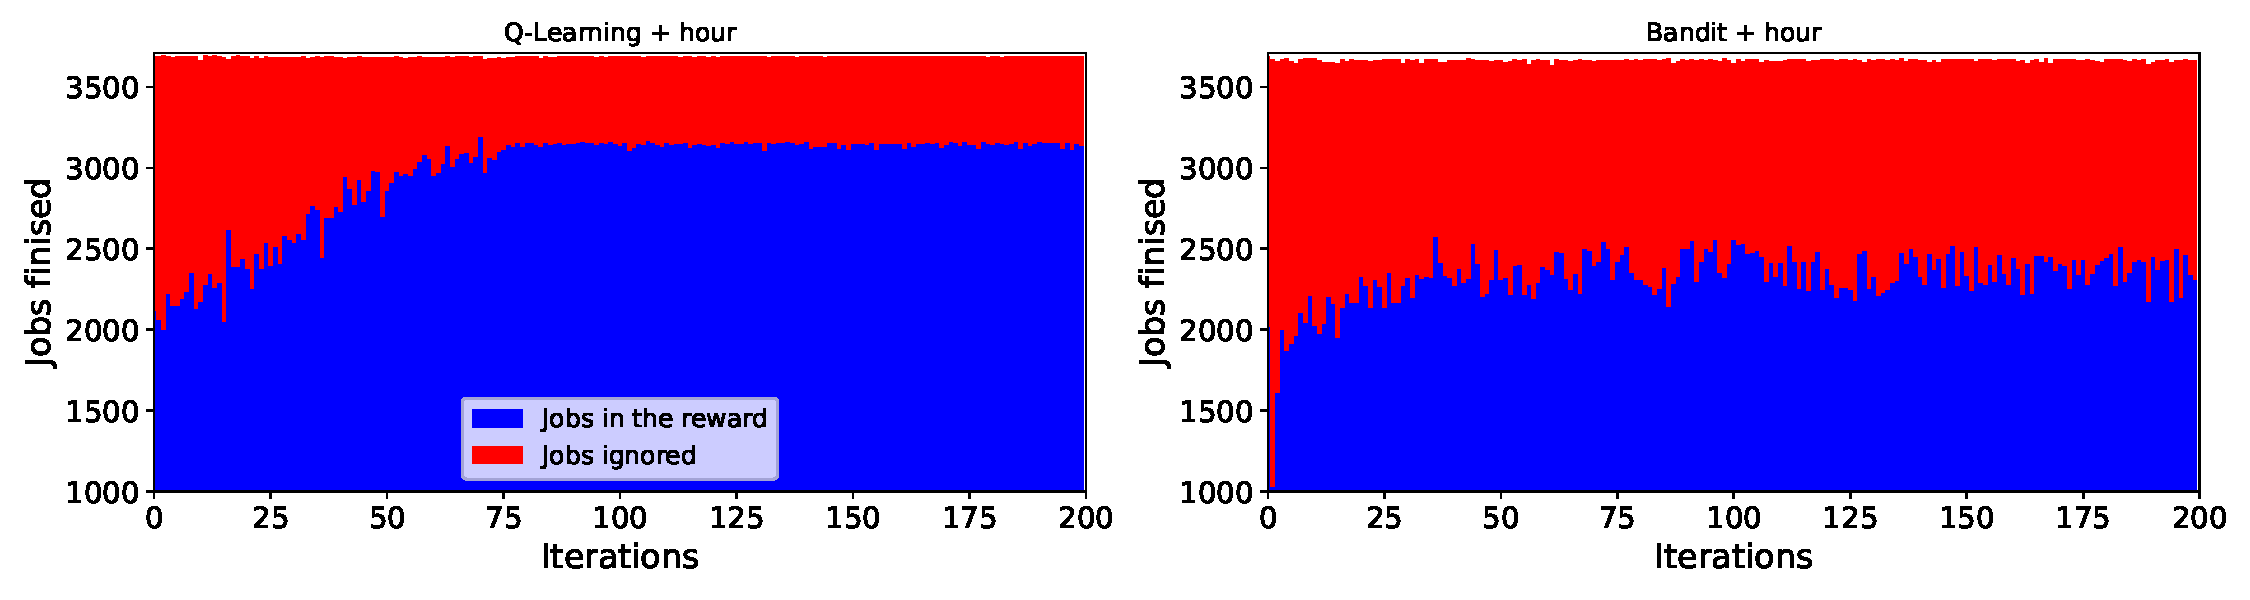
\includegraphics[scale=0.33]{Images/Learning_compensations/ignored_jobs_touched_scenario_1.pdf}
    \caption{The  jobs (finished and killed) included in the reward in critical case 1.}
    \label{fig:reward_from_jobs_critical_1}
\end{figure}

\begin{figure}[!htb]
    \centering
    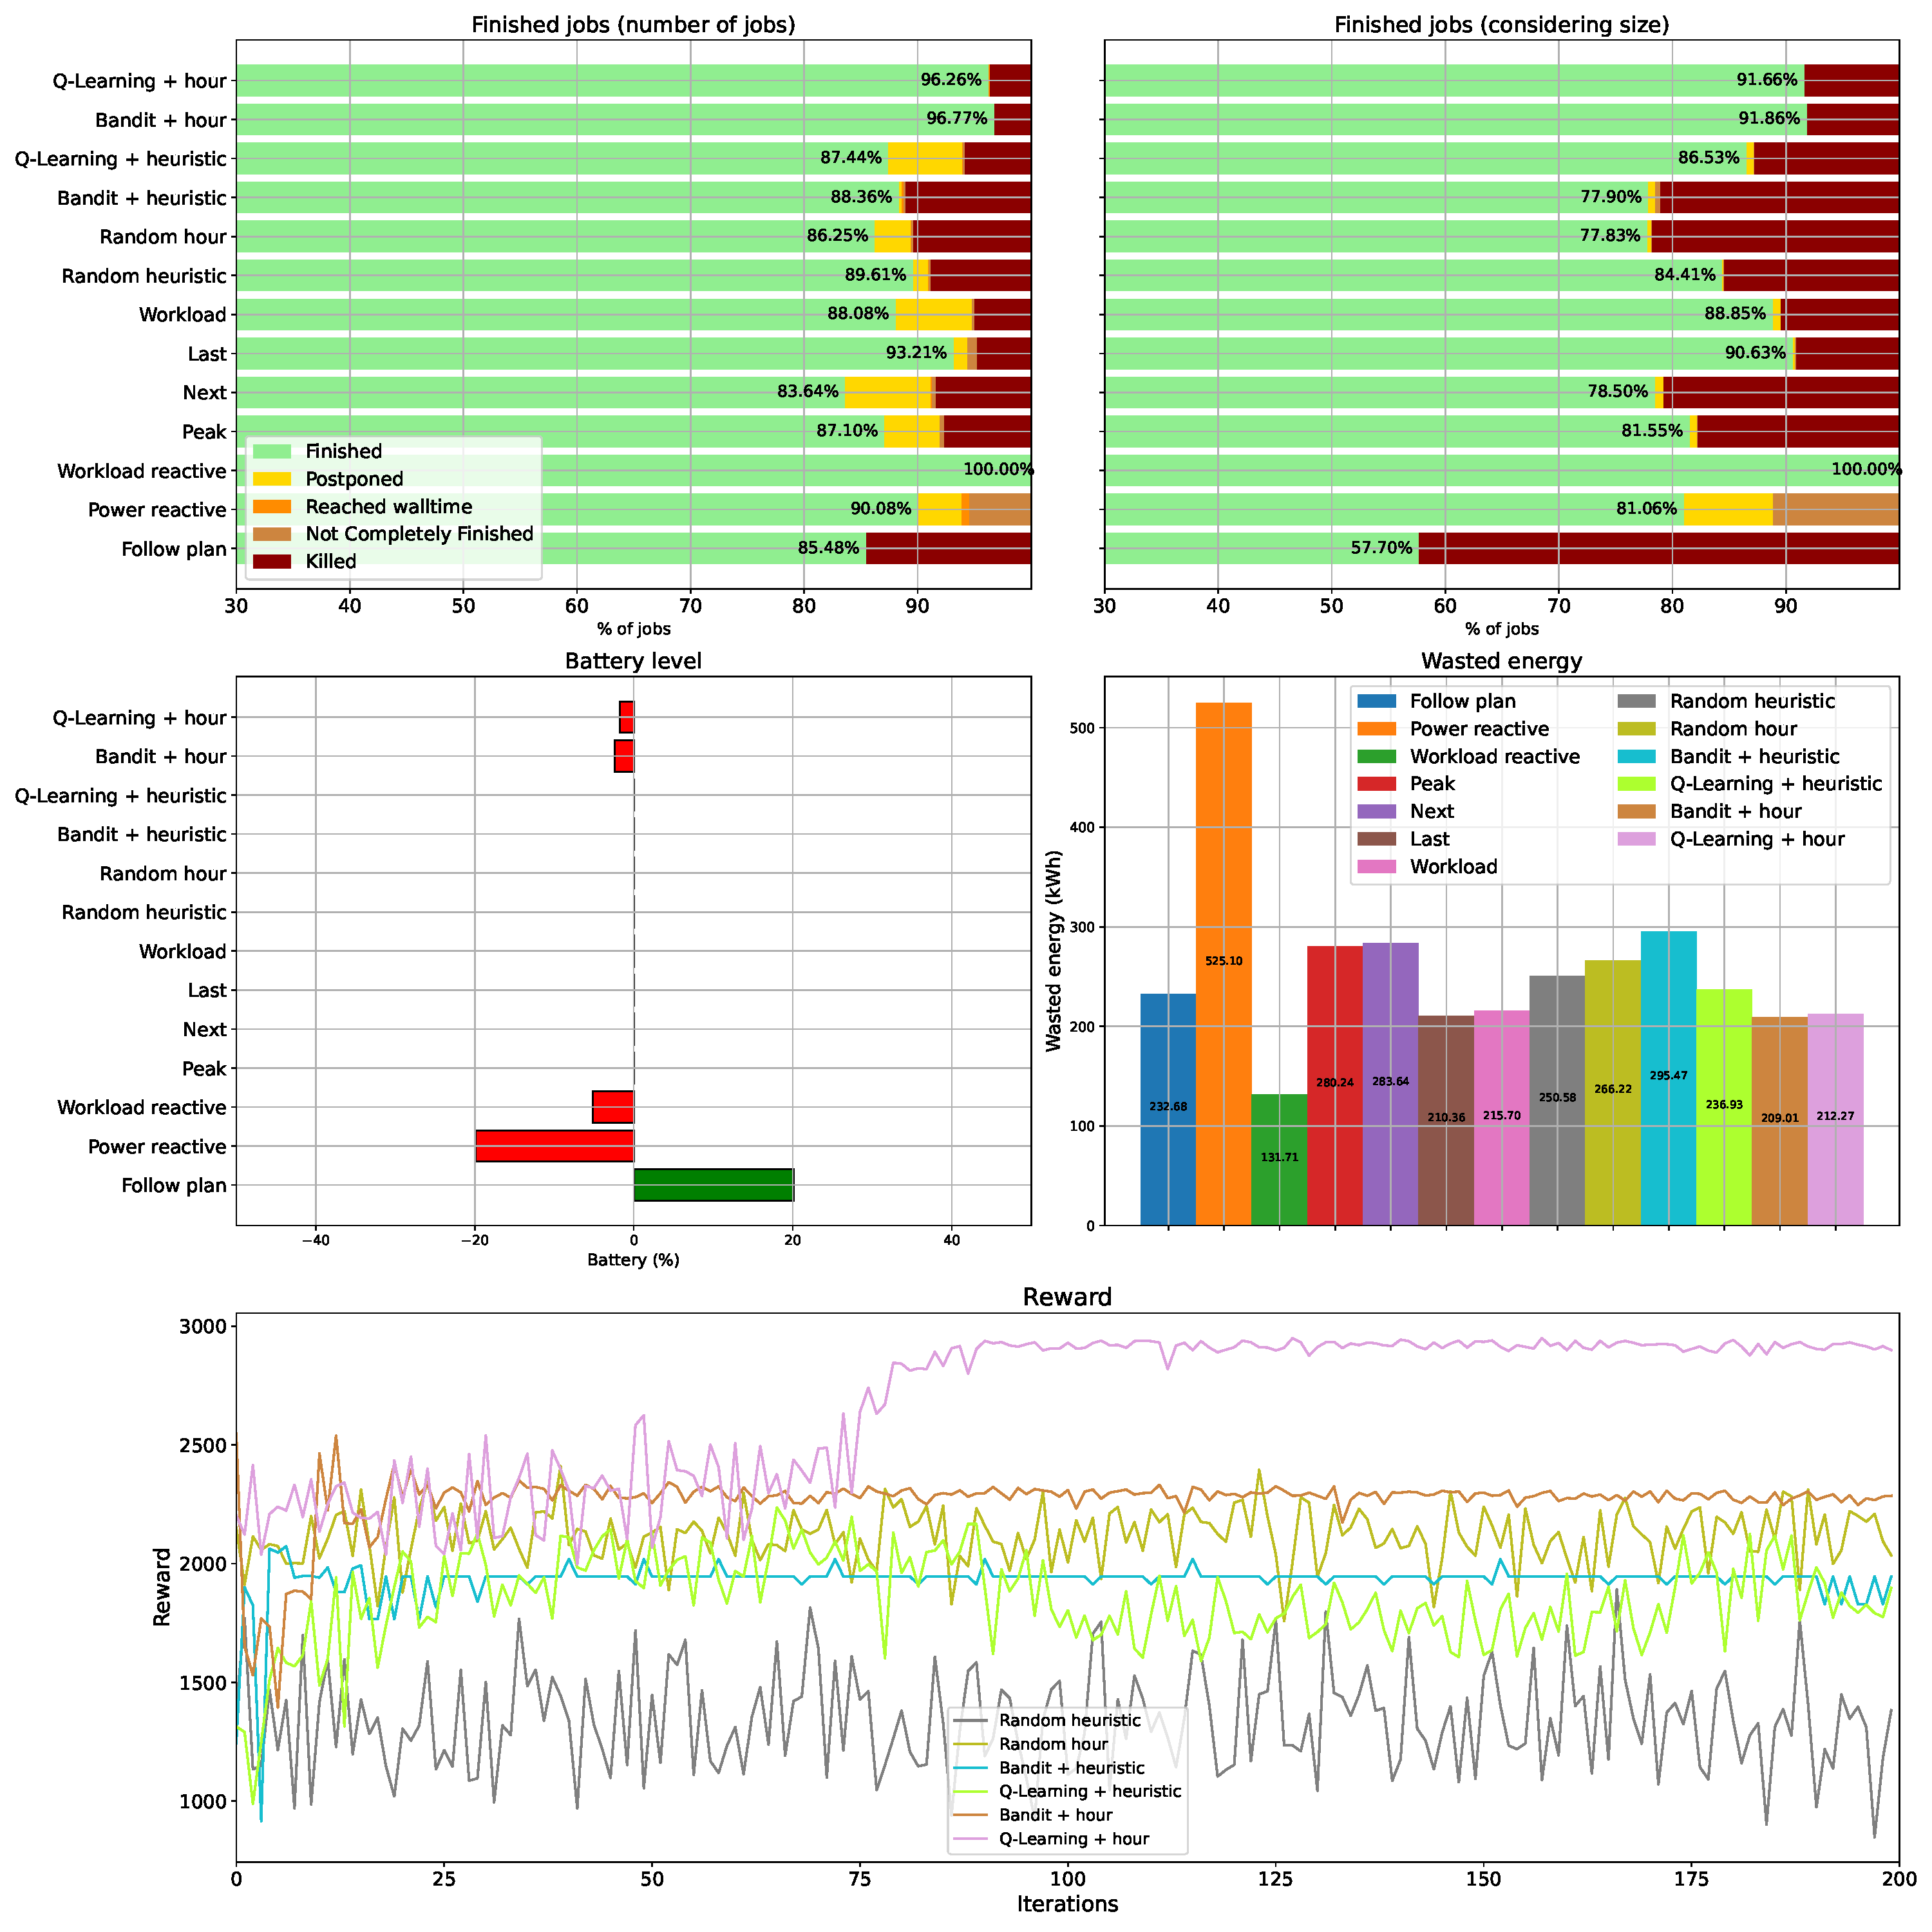
\includegraphics[scale=0.29]{Images/Learning_compensations/reward_finished_touched_profile_best_workload_2_with_noise_state_delta.pdf}
    \caption{Results of finished jobs reward in critical case 2.}
    \label{fig:touched_reward_results_critical_2}
\end{figure}

\begin{figure}[!htb]
    \centering
    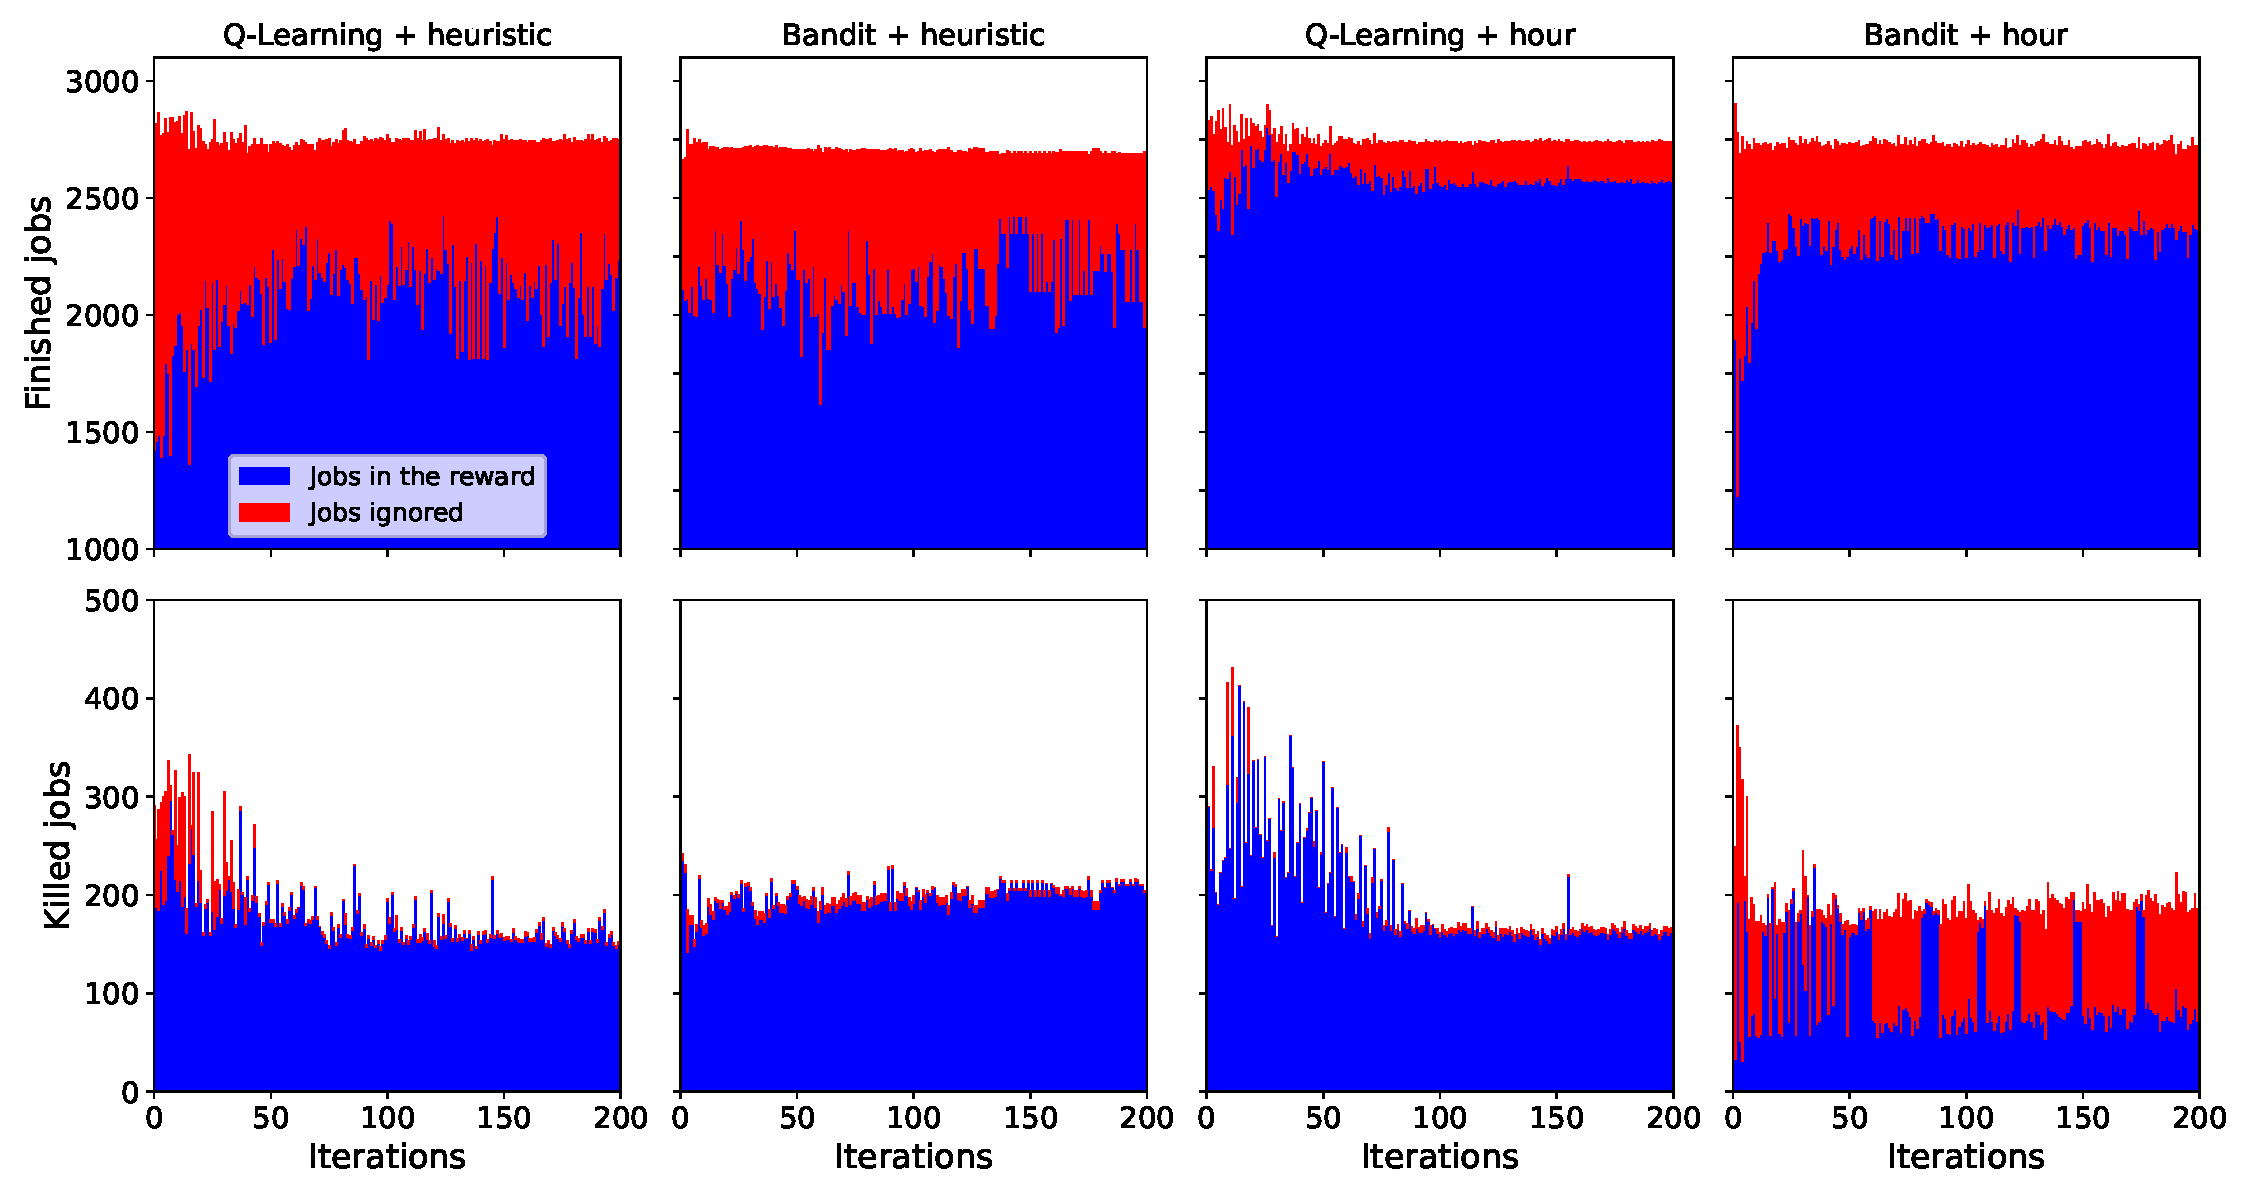
\includegraphics[scale=0.33]{Images/Learning_compensations/ignored_jobs_touched_scenario_2.pdf}
    \caption{The jobs (finished and killed) included in the reward in critical case 2.}
    \label{fig:reward_from_jobs_critical_2}
\end{figure}

Starting with critical case 1, Figure \ref{fig:touched_reward_results_critical_1} illustrates the results. The highest reward is from \emph{Q-Learning + hour}, which has the highest finished jobs in number and size among the RL algorithms. The second-best reward is \emph{Q-Learning + heuristic}, having also the second-best finished jobs (in number and size). However, we see a large difference between both rewards, which does not appear in the final finished jobs. Figure \ref{fig:reward_from_jobs_critical_1} highlights the problem. It is possible to notice that the reward's improvement of \emph{Q-Learning + hour} is not linked to more jobs finished, but due to more finished jobs included its reward. So, it puts energy into steps with more finished jobs just to receive the reward of them. \emph{Q-Learning + heuristic} "touches" fewer finished jobs, even finishing quite the same number of jobs. \emph{Q-Learning + heuristic}, \emph{Bandit + heuristic}, and \emph{Bandit + hour} do not increase the number of jobs finished, comparing the first iterations to the last ones, having constant finished jobs. Therefore, they do not improve the global finished jobs in this execution. \emph{Q-Learning + heuristic} is the only algorithm improving the global QoS comparing first iterations to the last ones (finished and killed jobs). Regarding the killed jobs, \emph{Q-Learning + hour} kills fewer jobs and almost every killed job is inside the reward. On the other hand, \emph{Q-Learning + heuristic} kills more jobs and has some killed jobs not included in the reward. Both Bandit algorithms have higher killed jobs and high reward variance, even in the last iterations. Going back to the results, \emph{Q-Learning + hour} presents quite the same result as the \emph{Last} policy in the number of finished jobs and lower finished jobs in size. Considering the battery, all RL algorithms are close to the target battery level. So, compared with \emph{Last}, the RL algorithms use more energy from the battery but not finishing more jobs. The wasted energy metric shows that the RL wasted more energy than the \emph{Last} policy. Hence, the more energy used by RL algorithms is wasted. We can observe that even doing a random algorithm is a good option in this scenario. \emph{Random step} has good finished jobs (in number), finishing more jobs than three of four RL algorithms. Furthermore, \emph{Random step} has the lowest wasted energy between random and RL algorithms.

Figure \ref{fig:touched_reward_results_critical_2} shows the results of critical case 2. In this scenario, \emph{Q-Learning + hour} has the highest reward, with \emph{Bandit + hour} being the second best. However, \emph{Q-Learning + heuristic} has the best number of finished jobs and killed jobs among the RL algorithms. Figure \ref{fig:reward_from_jobs_critical_2} shows that \emph{Q-Learning + hour} and \emph{Bandit + hour} touched more finished jobs than \emph{Q-Learning + heuristic}. Besides, \emph{Bandit + hour} touched less killed jobs. This algorithm "learns" to avoid some steps with killed jobs. So, it results in a higher reward, even with a lower QoS. Another important aspect is that \emph{Q-Learning + hour} reduces the number of finished jobs, comparing the first iterations to the last ones. This result indicates that this algorithm prefers to "touch" more finished jobs than finish more globally. Here, we can see that improving locally the reward does not mean that we will improve it globally. The same happened to \emph{Q-Learning + heuristic}. Going back to Figure \ref{fig:touched_reward_results_critical_2}, all RL algorithms are worst than \emph{Workload} and \emph{Last}, considering both finished and killed jobs. Even \emph{Random heuristic} is better than RL algorithms in finished jobs (in number), but it has higher killed jobs. Considering the battery level, the RL algorithm results are close to the target level. Finally, they wasted more energy than \emph{Last} and \emph{Workload} policies. 

\begin{figure}[!htb]
    \centering
    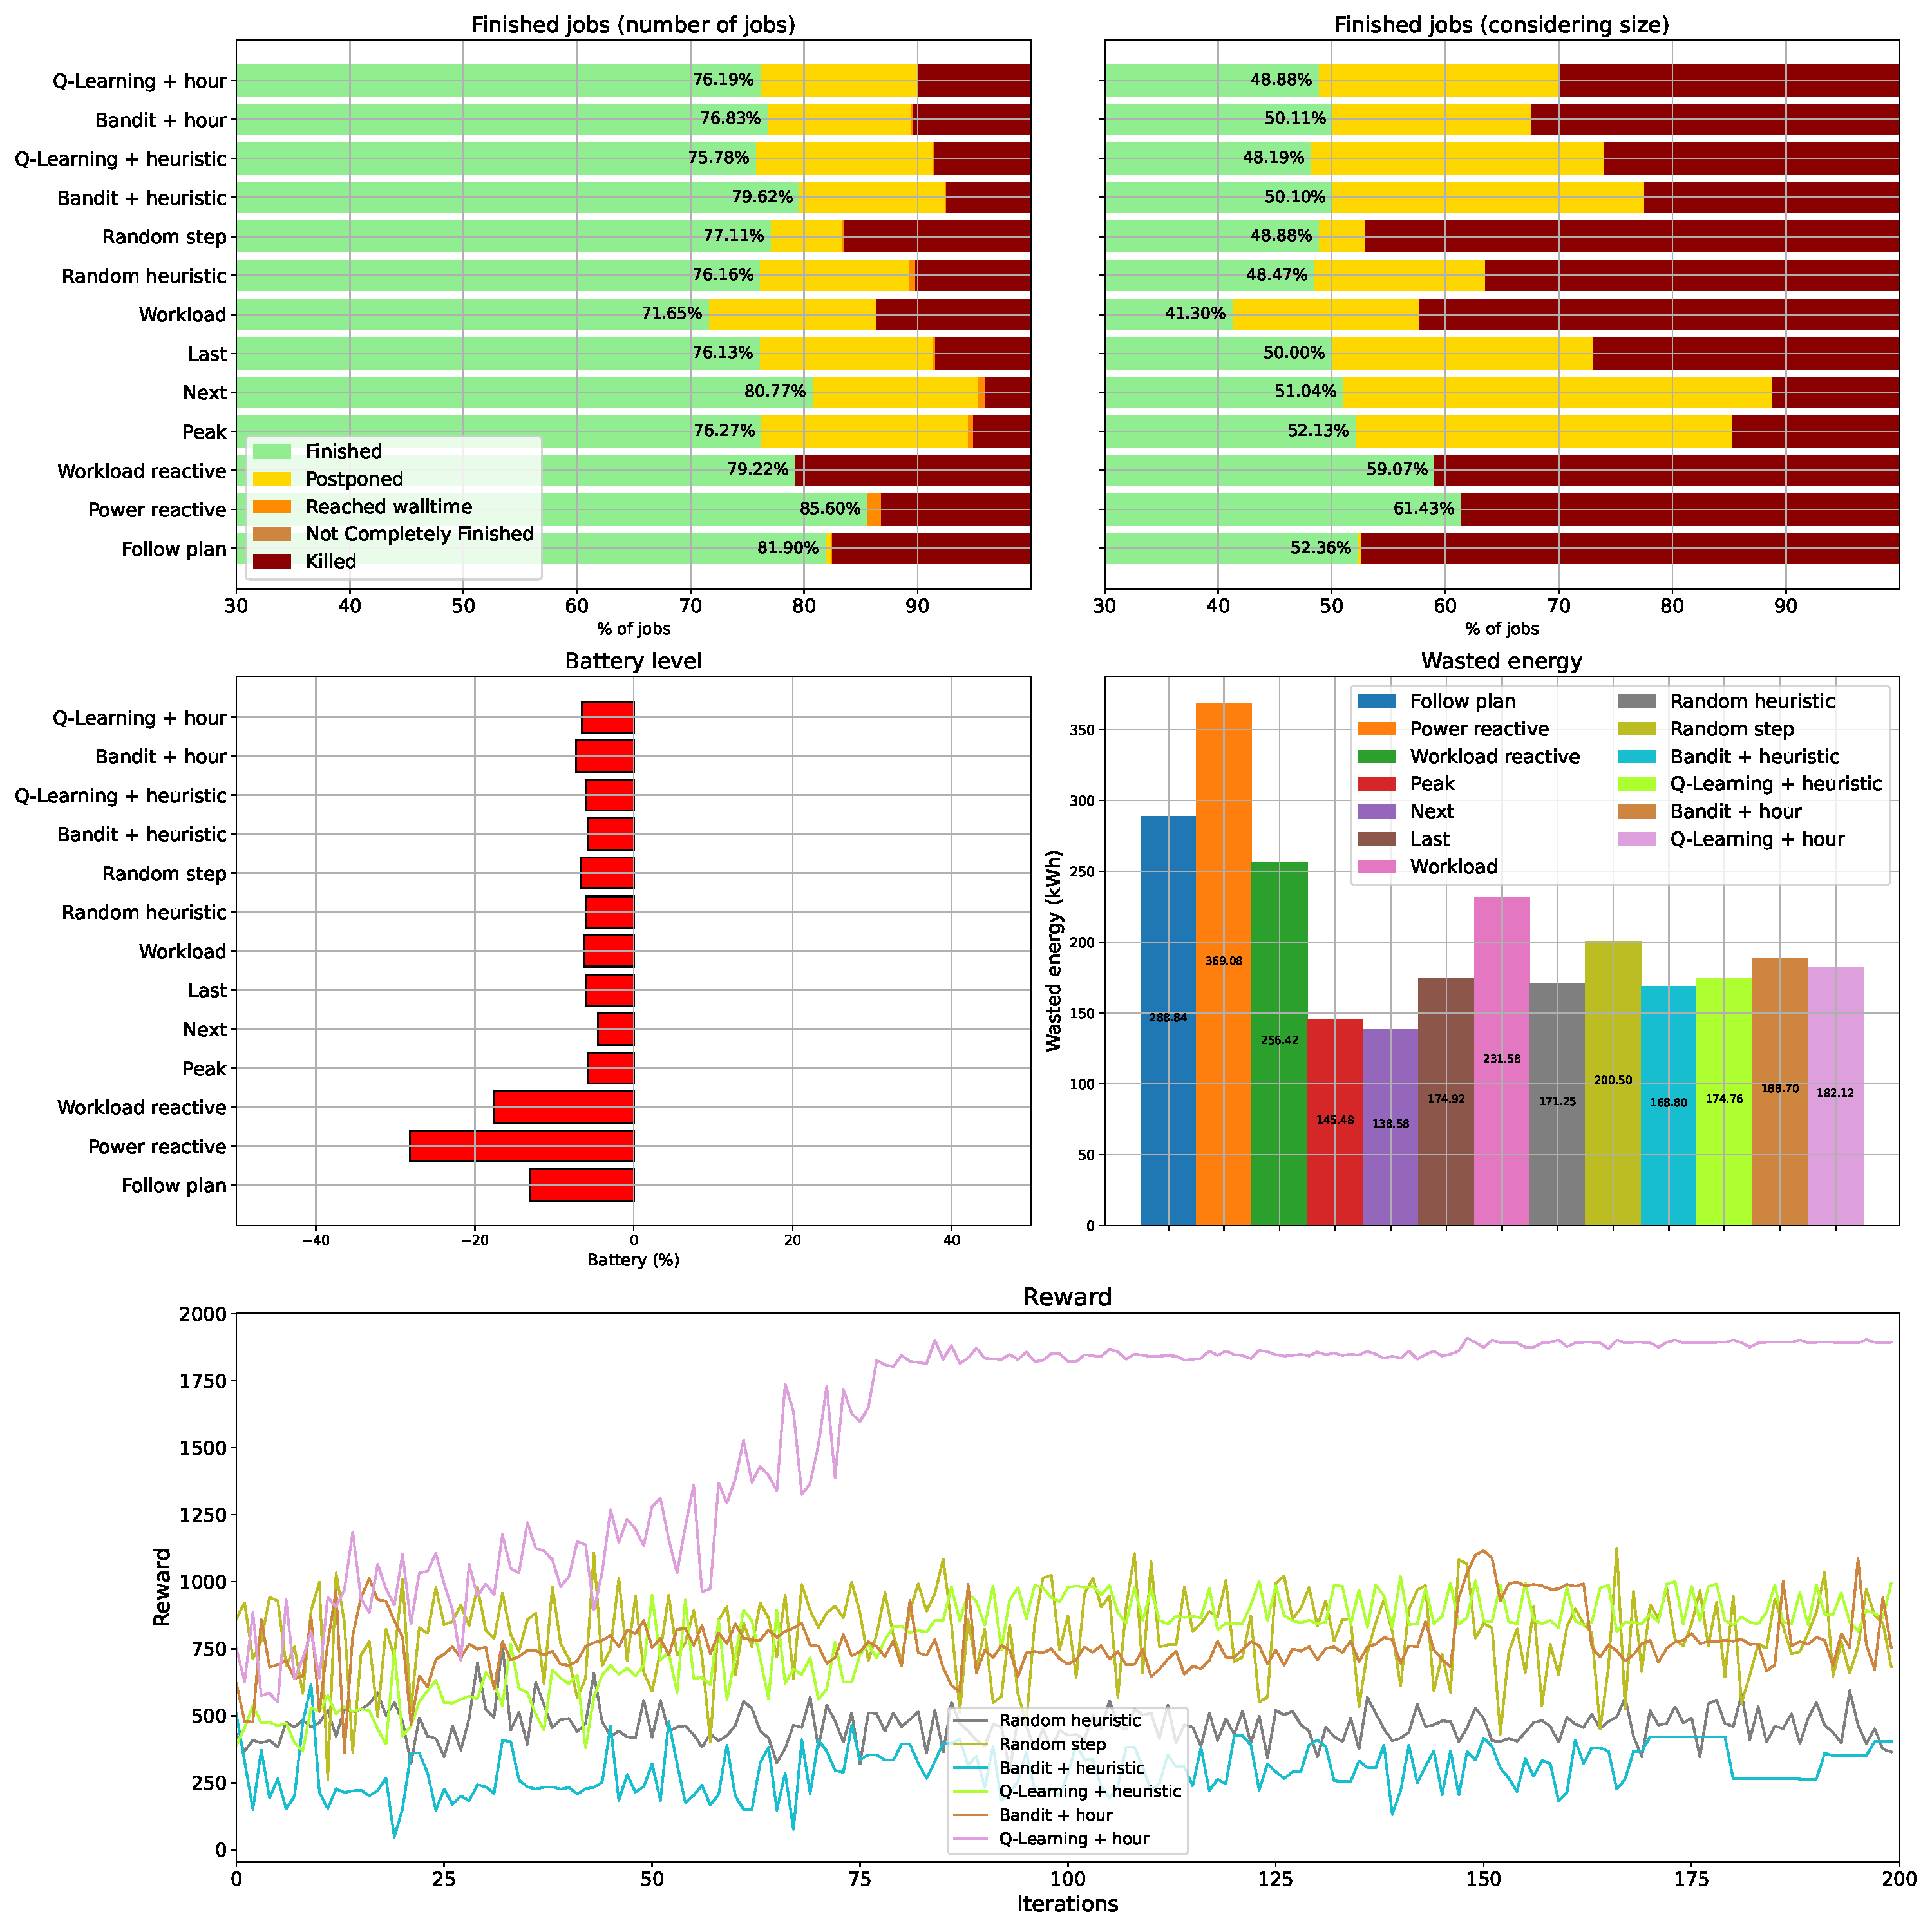
\includegraphics[scale=0.29]{Images/Learning_compensations/reward_finished_touched_profile_worst_workload_1_with_noise_state_delta.pdf}
    \caption{Results of finished jobs reward in critical case 3.}
    \label{fig:touched_reward_results_critical_3}
\end{figure}

\begin{figure}[!htb]
    \centering
    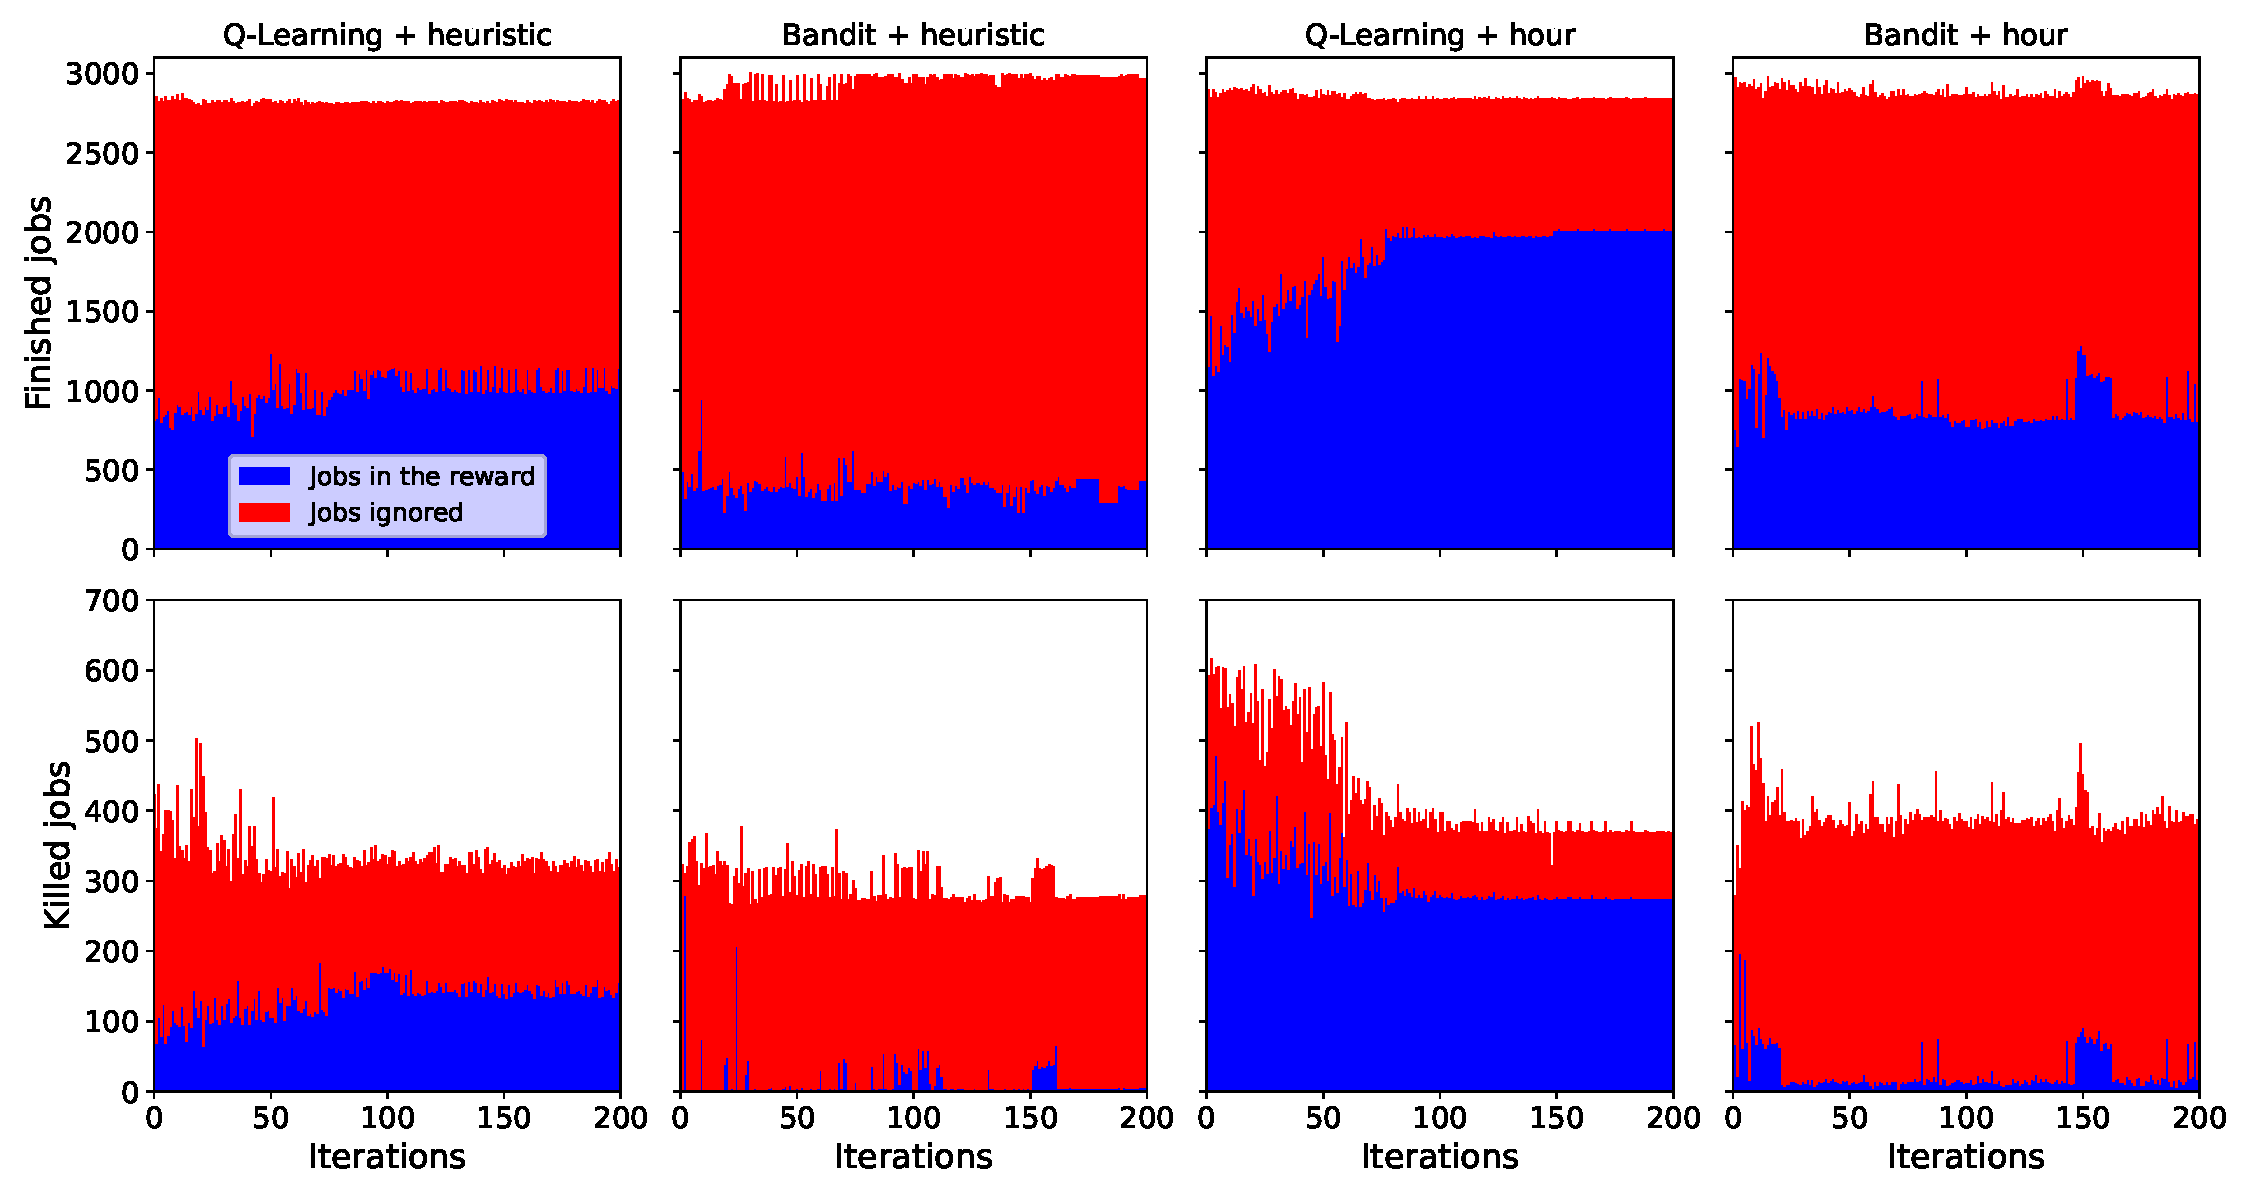
\includegraphics[scale=0.33]{Images/Learning_compensations/ignored_jobs_touched_scenario_3.pdf}
    \caption{The jobs (finished and killed) included in the reward in critical case 3.}
    \label{fig:reward_from_jobs_critical_3}
\end{figure}

Starting the cases with less energy, Figure \ref{fig:touched_reward_results_critical_3} shows the results of critical case 3. \emph{Q-Learning + hour} has the best reward but is not the best algorithm in finished/killed jobs metrics. The best result comes from \emph{Bandit + heuristic}, with the highest number of finished jobs and the lowest number of killed jobs among the RL algorithms. However, \emph{Bandit + heuristic} has the lowest reward. Figure \ref{fig:reward_from_jobs_critical_3} shows a higher global number of finished jobs and lower killed jobs in \emph{Bandit + heuristic} compared to the other algorithms. So, we can see that doing good local decisions does not mean good global results in our problem. Both \emph{Q-Learning + hour} touched more jobs than \emph{Bandit + heuristic}, increasing their reward. However, \emph{Q-Learning + hour} increases the number of touched finished jobs, which leads to a reduction in the global finished jobs. At least, this algorithm arrives to reduce the number of killed jobs in this scenario. Coming back to Figure \ref{fig:touched_reward_results_critical_3}, no RL is better than \emph{Next} policy in number of finished jobs and better than \emph{Peak} policy in size of finished jobs. Both \emph{Next} and \emph{Peak} are still the executions with the lowest killed jobs. Both random algorithms kill several jobs. So, random is not an option either. Considering the battery level, all RL algorithm results are close to the policies. Regarding wasted energy, all RL algorithms wasted more than \emph{Peak} and \emph{Next} policies. This scenario shows that even including QoS decisions in the algorithm, a renewable-only data center demands better battery management, like \emph{Next} policy. Maintaining the QoS above $SoC_{min}$ is the most important constraint in a scenario with less energy.

\begin{figure}[!htb]
    \centering
    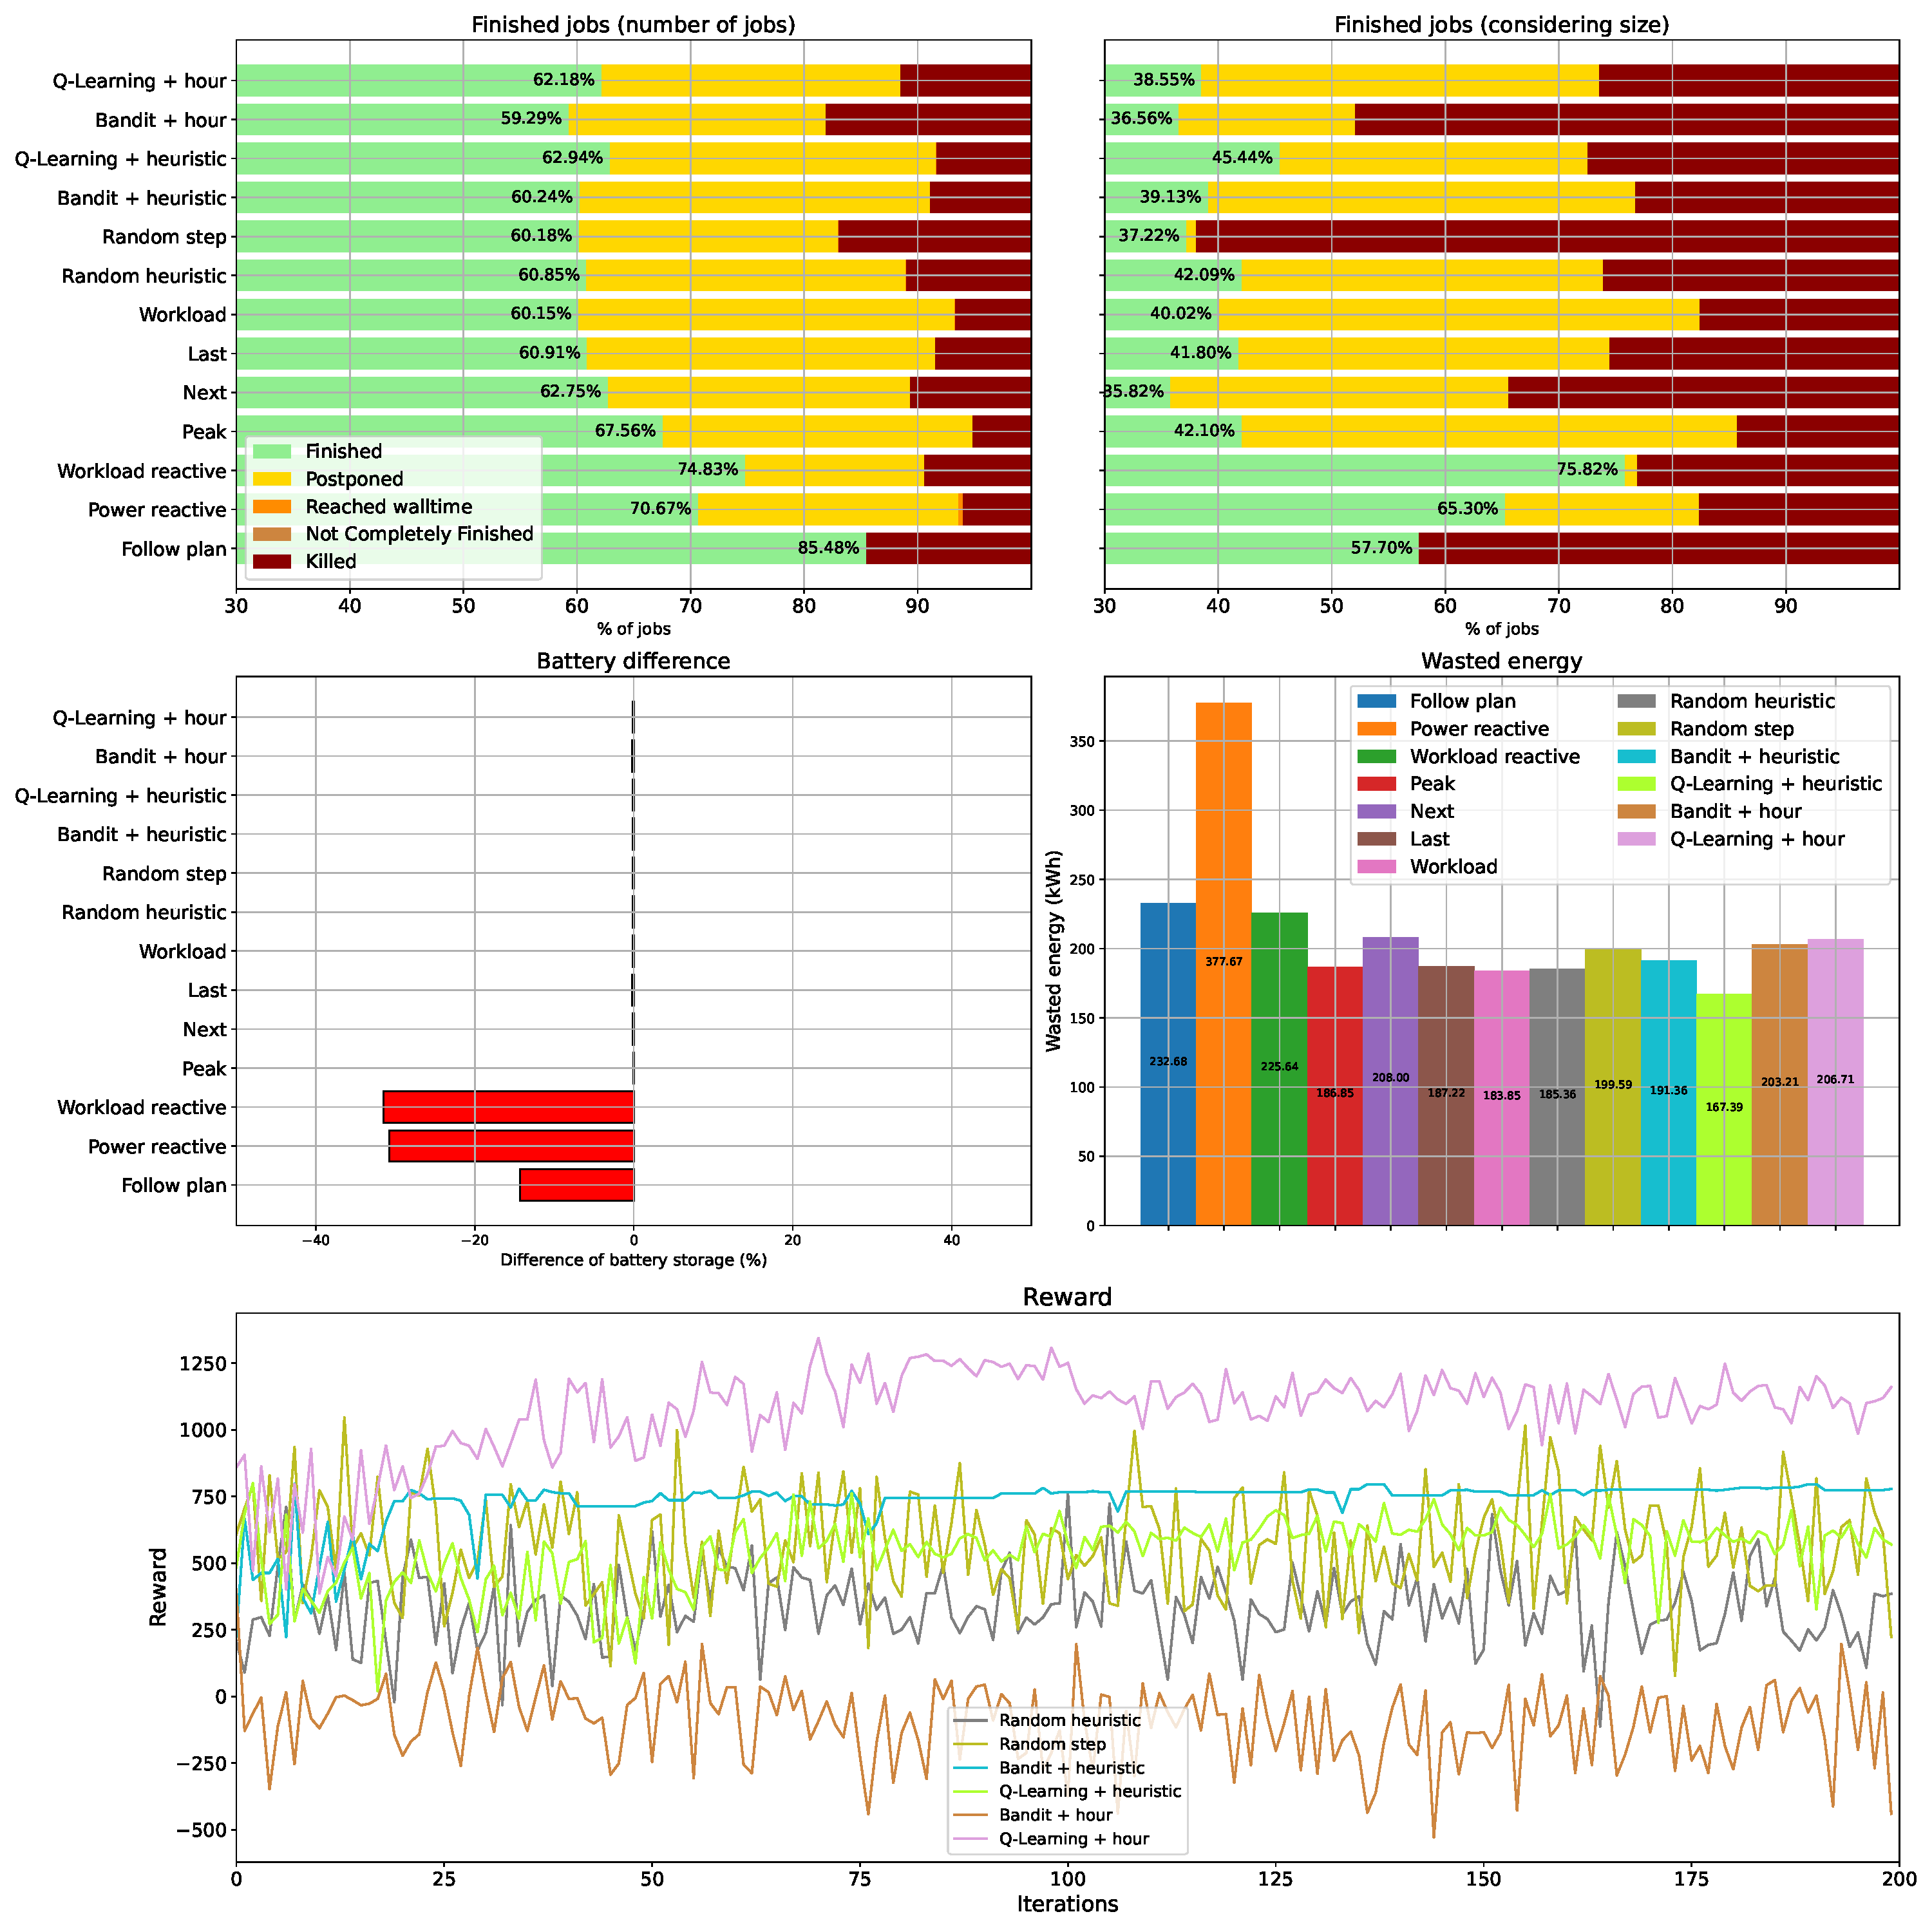
\includegraphics[scale=0.29]{Images/Learning_compensations/reward_finished_touched_profile_worst_workload_2_with_noise_state_delta.pdf}
    \caption{Results of finished jobs reward in critical case 4.}
    \label{fig:touched_reward_results_critical_4}
\end{figure}

\begin{figure}[!htb]
    \centering
    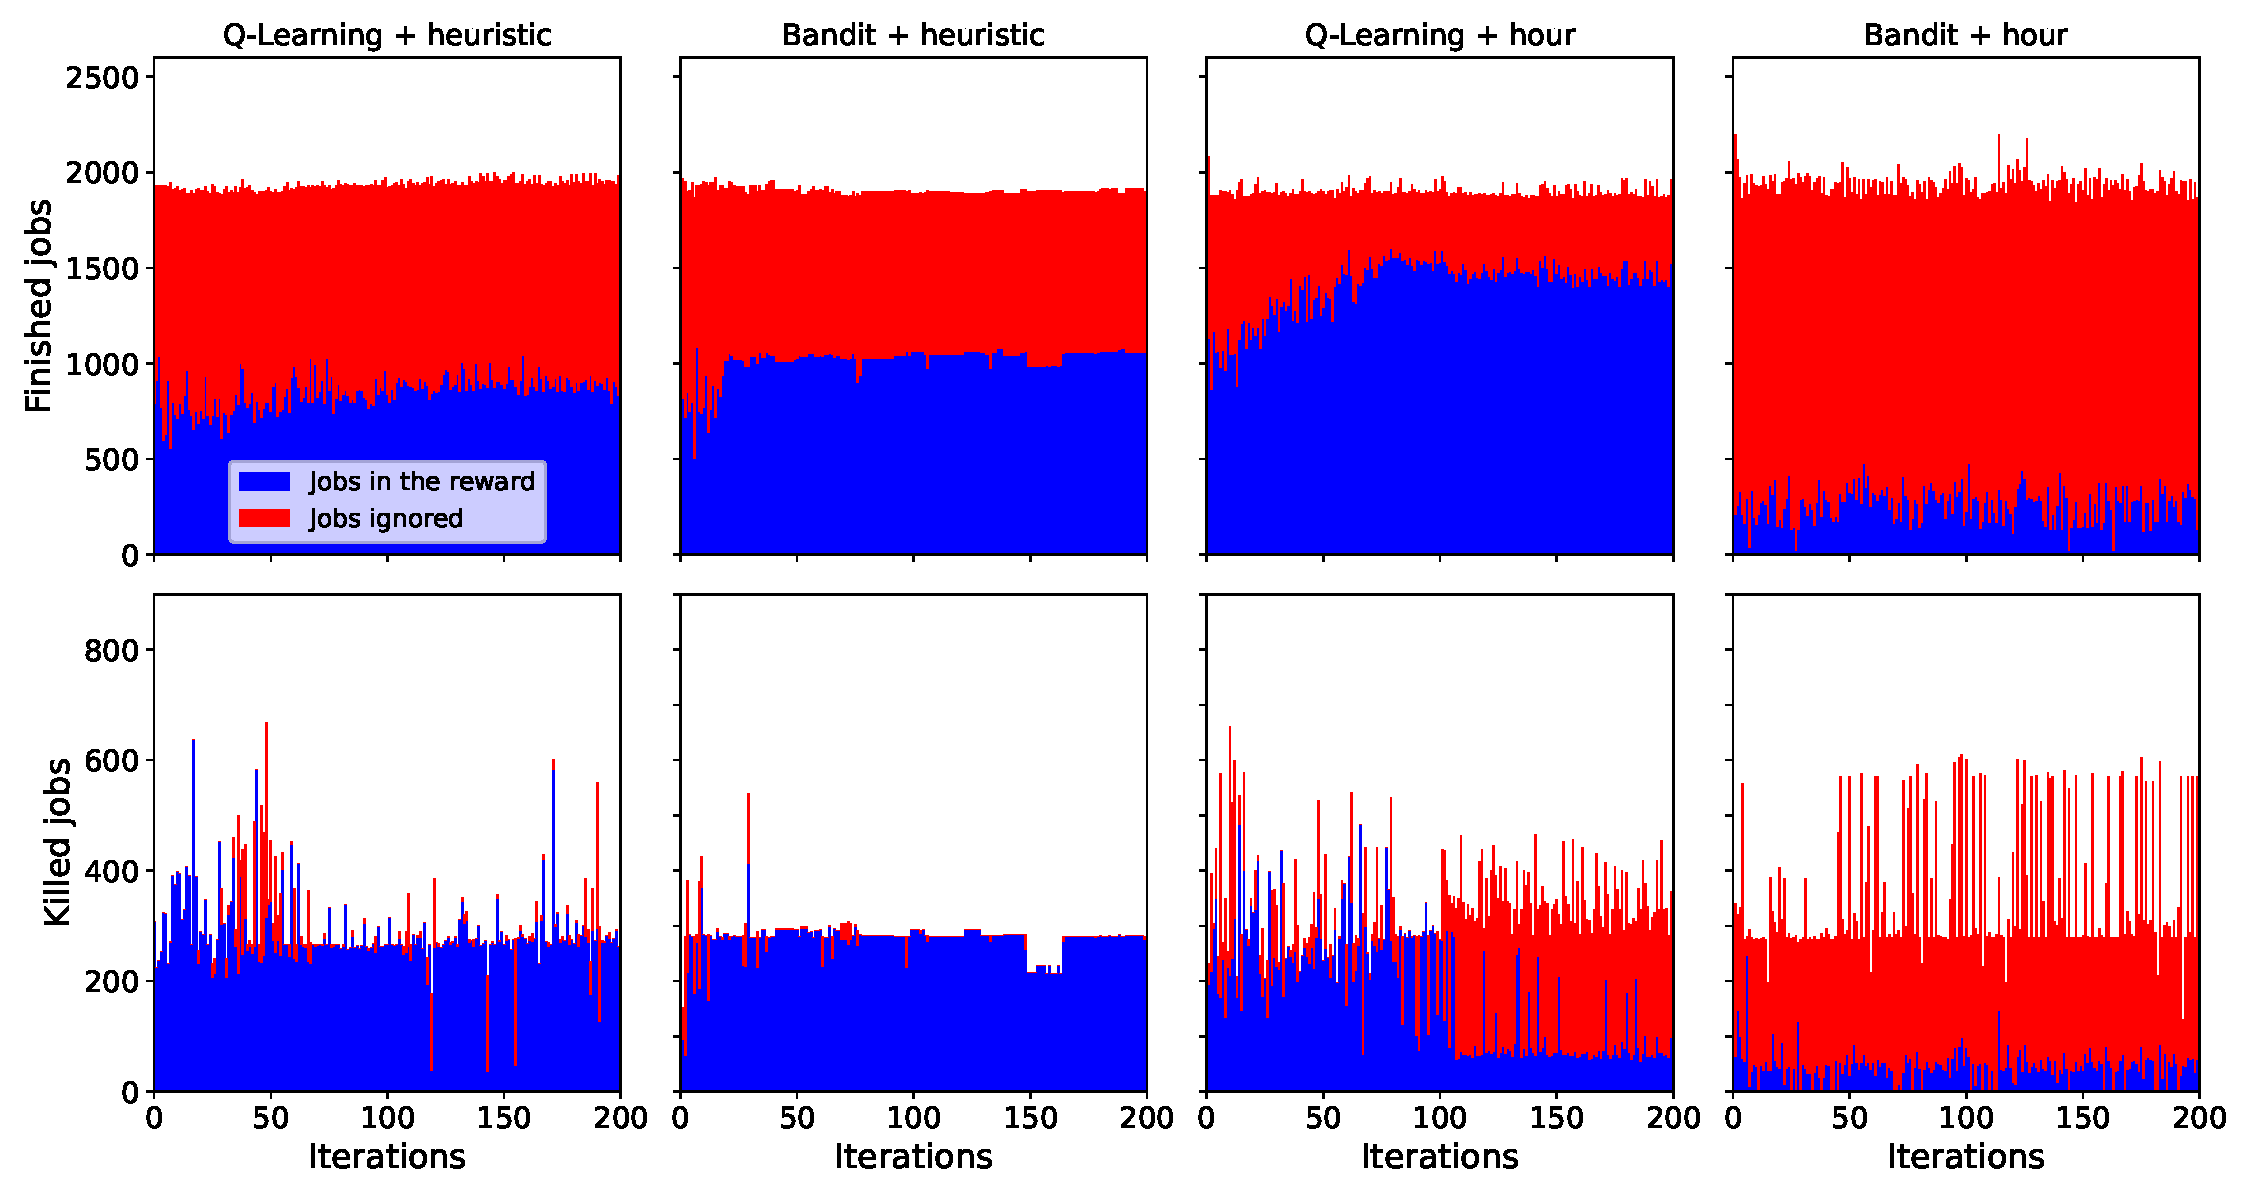
\includegraphics[scale=0.33]{Images/Learning_compensations/ignored_jobs_touched_scenario_4.pdf}
    \caption{The jobs (finished and killed) included in the reward in critical case 4.}
    \label{fig:reward_from_jobs_critical_4}
\end{figure}

Finally, the last results of critical case 4 are presented in Figure \ref{fig:touched_reward_results_critical_4}. This scenario also has less energy arriving. We can see that \emph{Q-Learning + hour} has the highest reward. It also has the second-best finished jobs among the RL. Again, the highest number of finished jobs come from the RL with not the highest reward, \emph{Q-Learning + heuristic}. Figure \ref{fig:reward_from_jobs_critical_4} illustrates that \emph{Q-Learning + heuristic} touches fewer jobs than \emph{Q-Learning + hour}, but finishes more. This shows again that the best local decisions (see the reward obtained by \emph{Q-Learning + hour}) do not improve the global QoS. In this case, \emph{Q-Learning + hour} improves more jobs but increases the number of killed jobs. It avoids the steps with these killed jobs, increasing its reward. However, both \emph{Q-Learning + hour} and \emph{Bandit + hour} do not stabilize the number of killed jobs, having high variation even in later iterations. Returning to Figure \ref{fig:touched_reward_results_critical_4}, \emph{Q-Learning + heuristic} has the best finished jobs considering the size, even better than the policies. However, it also kills more than \emph{Peak} and \emph{Workload}. Considering the battery level, again, all the RL algorithms are close to the target level. Finally, the \emph{Q-Learning + heuristic} presents the lowest wasted energy. This result is linked to the finished jobs considering the size, where this algorithm finished more than all policies. So, this algorithm arrives to maintain more big jobs running for longer, using the energy well.

Similarly to the previous reward, Table \ref{tab:ranking_finished} presents the final metrics of the algorithms. Again, the RL algorithms do not improve the results, having just some metrics at the top 3 and some at the bottom 3. The results majority of RL algorithms stay out of the top 3 and bottom 3 ranking. After presenting all results, Section \ref{sec:learning_discussion} discusses them more generally, indicating the problems of our RL model and proposing future possibilities in machine learning.

% Please add the following required packages to your document preamble:
% \usepackage{multirow}

\begin{landscape}

\mbox{}\vfill

\begin{table*}[htp]
    \centering
    \caption{Consolidate average results in every scenario for reward finished.}
    \label{tab:ranking_finished}
    \scriptsize
    \begin{tabular}{c|l||l|l|l|l|l|l|l|l|l|l|l|l|l}
    \hline
    Scenario & Metric & \begin{tabular}[c]{@{}l@{}}Follow \\ plan\end{tabular} & \begin{tabular}[c]{@{}l@{}}Power \\ reactive\end{tabular} & \begin{tabular}[c]{@{}l@{}}Workload\\ reactive\end{tabular} & Peak & Next & Last & Load & \begin{tabular}[c]{@{}l@{}}Rand.\\ heur.\end{tabular} & \begin{tabular}[c]{@{}l@{}}Rand.\\ step\end{tabular} & \begin{tabular}[c]{@{}l@{}}Bandit + \\ heuristic\end{tabular} & \begin{tabular}[c]{@{}l@{}}Q-Learn. + \\ heuristic\end{tabular} & \begin{tabular}[c]{@{}l@{}}Bandit + \\ hour\end{tabular} & \begin{tabular}[c]{@{}l@{}}Q-Learn. + \\ hour\end{tabular} \\ \hline\hline
    \multirow{4}{*}{\begin{tabular}[c]{@{}c@{}}Profile best-case \\ and \\ workload in \\ beginning\end{tabular}} & Finished jobs & {\cellcolor{red!75}}\nth{13} & {\cellcolor{red!50}}\nth{12} & {\cellcolor{red!25}}\nth{11} & \nth{9} & \nth{10} & {\cellcolor{green!75}}\nth{1} & \nth{5} & \nth{8} & {\cellcolor{green!25}}\nth{3} & \nth{7} & \nth{4} & \nth{6} & {\cellcolor{green!50}}\nth{2} \\ \cline{2-15} 
     & Killed jobs & {\cellcolor{red!75}}\nth{13} & {\cellcolor{red!50}}\nth{12} & {\cellcolor{red!25}}\nth{11} & \nth{9} & \nth{10} & {\cellcolor{green!75}}\nth{1} & \nth{5} & \nth{8} & {\cellcolor{green!25}}\nth{3} & \nth{7} & \nth{4} & \nth{6} & {\cellcolor{green!50}}\nth{2} \\ \cline{2-15} 
     & SoC & {\cellcolor{green!75}}\nth{1} & {\cellcolor{red!75}}\nth{13} & {\cellcolor{green!50}}\nth{2} & \nth{10} & {\cellcolor{red!50}}\nth{12} & {\cellcolor{green!25}}\nth{3} & \nth{7} & \nth{4} & \nth{5} & {\cellcolor{red!25}}\nth{11} & \nth{8} & \nth{9} & \nth{6} \\ \cline{2-15} 
     & Wasted energy & {\cellcolor{red!50}}\nth{12} & {\cellcolor{red!75}}\nth{13} & {\cellcolor{green!75}}\nth{1} & \nth{7} & \nth{10} & {\cellcolor{green!50}}\nth{2} & \nth{8} & \nth{6} & {\cellcolor{green!25}}\nth{3} & {\cellcolor{red!25}}\nth{11} & \nth{5} & \nth{9} & \nth{4} \\ \hline\hline
    \multirow{4}{*}{\begin{tabular}[c]{@{}c@{}}Profile best-case \\ and \\ workload in end\end{tabular}} & Finished jobs & {\cellcolor{red!50}}\nth{12} & {\cellcolor{green!25}}\nth{3} & {\cellcolor{green!75}}\nth{1} & \nth{7} & {\cellcolor{red!75}}\nth{13} & {\cellcolor{green!50}}\nth{2} & \nth{5} & \nth{4} & \nth{10} & {\cellcolor{red!25}}\nth{11} & \nth{6} & \nth{9} & \nth{8} \\ \cline{2-15} 
     & Killed jobs & {\cellcolor{red!75}}\nth{13} & \nth{7} & {\cellcolor{green!75}}\nth{1} & \nth{9} & \nth{10} & \nth{5} & {\cellcolor{green!25}}\nth{3} & {\cellcolor{red!25}}\nth{11} & {\cellcolor{red!50}}\nth{12} & \nth{8} & {\cellcolor{green!50}}\nth{2} & \nth{6} & \nth{4} \\ \cline{2-15} 
     & SoC & {\cellcolor{green!75}}\nth{1} & {\cellcolor{red!75}}\nth{13} & {\cellcolor{red!50}}\nth{12} & {\cellcolor{green!25}}\nth{3} & \nth{4} & \nth{6} & \nth{7} & {\cellcolor{green!50}}\nth{2} & \nth{9} & \nth{8} & \nth{10} & \nth{5} & {\cellcolor{red!25}}\nth{11} \\ \cline{2-15} 
     & Wasted energy & \nth{5} & {\cellcolor{red!75}}\nth{13} & {\cellcolor{green!75}}\nth{1} & {\cellcolor{red!25}}\nth{11} & {\cellcolor{red!50}}\nth{12} & {\cellcolor{green!50}}\nth{2} & {\cellcolor{green!25}}\nth{3} & \nth{8} & \nth{10} & \nth{9} & \nth{4} & \nth{7} & \nth{6} \\ \hline\hline
    \multirow{4}{*}{\begin{tabular}[c]{@{}c@{}}Profile worst-case \\ and \\ workload in \\ beginning\end{tabular}} & Finished jobs & {\cellcolor{green!50}}\nth{2} & {\cellcolor{green!75}}\nth{1} & \nth{5} & \nth{8} & {\cellcolor{green!25}}\nth{3} & {\cellcolor{red!25}}\nth{11} & {\cellcolor{red!75}}\nth{13} & \nth{10} & \nth{6} & \nth{4} & {\cellcolor{red!50}}\nth{12} & \nth{7} & \nth{9} \\ \cline{2-15} 
     & Killed jobs & {\cellcolor{red!50}}\nth{12} & \nth{10} & {\cellcolor{red!75}}\nth{13} & {\cellcolor{green!50}}\nth{2} & {\cellcolor{green!75}}\nth{1} & \nth{5} & \nth{9} & \nth{8} & {\cellcolor{red!25}}\nth{11} & {\cellcolor{green!25}}\nth{3} & \nth{4} & \nth{7} & \nth{6} \\ \cline{2-15} 
     & SoC & {\cellcolor{red!25}}\nth{11} & {\cellcolor{red!75}}\nth{13} & {\cellcolor{red!50}}\nth{12} & {\cellcolor{green!25}}\nth{3} & {\cellcolor{green!75}}\nth{1} & \nth{4} & \nth{7} & \nth{6} & \nth{9} & {\cellcolor{green!50}}\nth{2} & \nth{5} & \nth{10} & \nth{8} \\ \cline{2-15} 
     & Wasted energy & {\cellcolor{red!50}}\nth{12} & {\cellcolor{red!75}}\nth{13} & {\cellcolor{red!25}}\nth{11} & {\cellcolor{green!50}}\nth{2} & {\cellcolor{green!75}}\nth{1} & \nth{6} & \nth{10} & \nth{4} & \nth{9} & {\cellcolor{green!25}}\nth{3} & \nth{5} & \nth{8} & \nth{7} \\ \hline\hline
    \multirow{4}{*}{\begin{tabular}[c]{@{}c@{}}Profile worst-case \\ and \\ workload in end\end{tabular}} & Finished jobs & {\cellcolor{green!75}}\nth{1} & {\cellcolor{green!25}}\nth{3} & {\cellcolor{green!50}}\nth{2} & \nth{4} & \nth{6} & \nth{8} & {\cellcolor{red!50}}\nth{12} & \nth{9} & {\cellcolor{red!25}}\nth{11} & \nth{10} & \nth{5} & {\cellcolor{red!75}}\nth{13} & \nth{7} \\ \cline{2-15} 
     & Killed jobs & {\cellcolor{red!25}}\nth{11} & {\cellcolor{green!50}}\nth{2} & \nth{7} & {\cellcolor{green!75}}\nth{1} & \nth{8} & \nth{5} & {\cellcolor{green!25}}\nth{3} & \nth{9} & {\cellcolor{red!50}}\nth{12} & \nth{6} & \nth{4} & {\cellcolor{red!75}}\nth{13} & \nth{10} \\ \cline{2-15} 
     & SoC & {\cellcolor{red!25}}\nth{11} & {\cellcolor{red!50}}\nth{12} & {\cellcolor{red!75}}\nth{13} & {\cellcolor{green!75}}\nth{1} & {\cellcolor{green!50}}\nth{2} & \nth{10} & \nth{4} & \nth{7} & \nth{6} & \nth{5} & \nth{8} & \nth{9} & {\cellcolor{green!25}}\nth{3} \\ \cline{2-15} 
     & Wasted energy & {\cellcolor{red!50}}\nth{12} & {\cellcolor{red!75}}\nth{13} & {\cellcolor{red!25}}\nth{11} & \nth{4} & \nth{10} & \nth{5} & {\cellcolor{green!50}}\nth{2} & {\cellcolor{green!25}}\nth{3} & \nth{7} & \nth{6} & {\cellcolor{green!75}}\nth{1} & \nth{8} & \nth{9} \\ \hline
    \end{tabular}
\end{table*}

\vfill
\end{landscape}

\clearpage


% \clearpage

% \subsection{Finished Jobs Spread Reward}

% \begin{figure}[!htb]
%     \centering
%     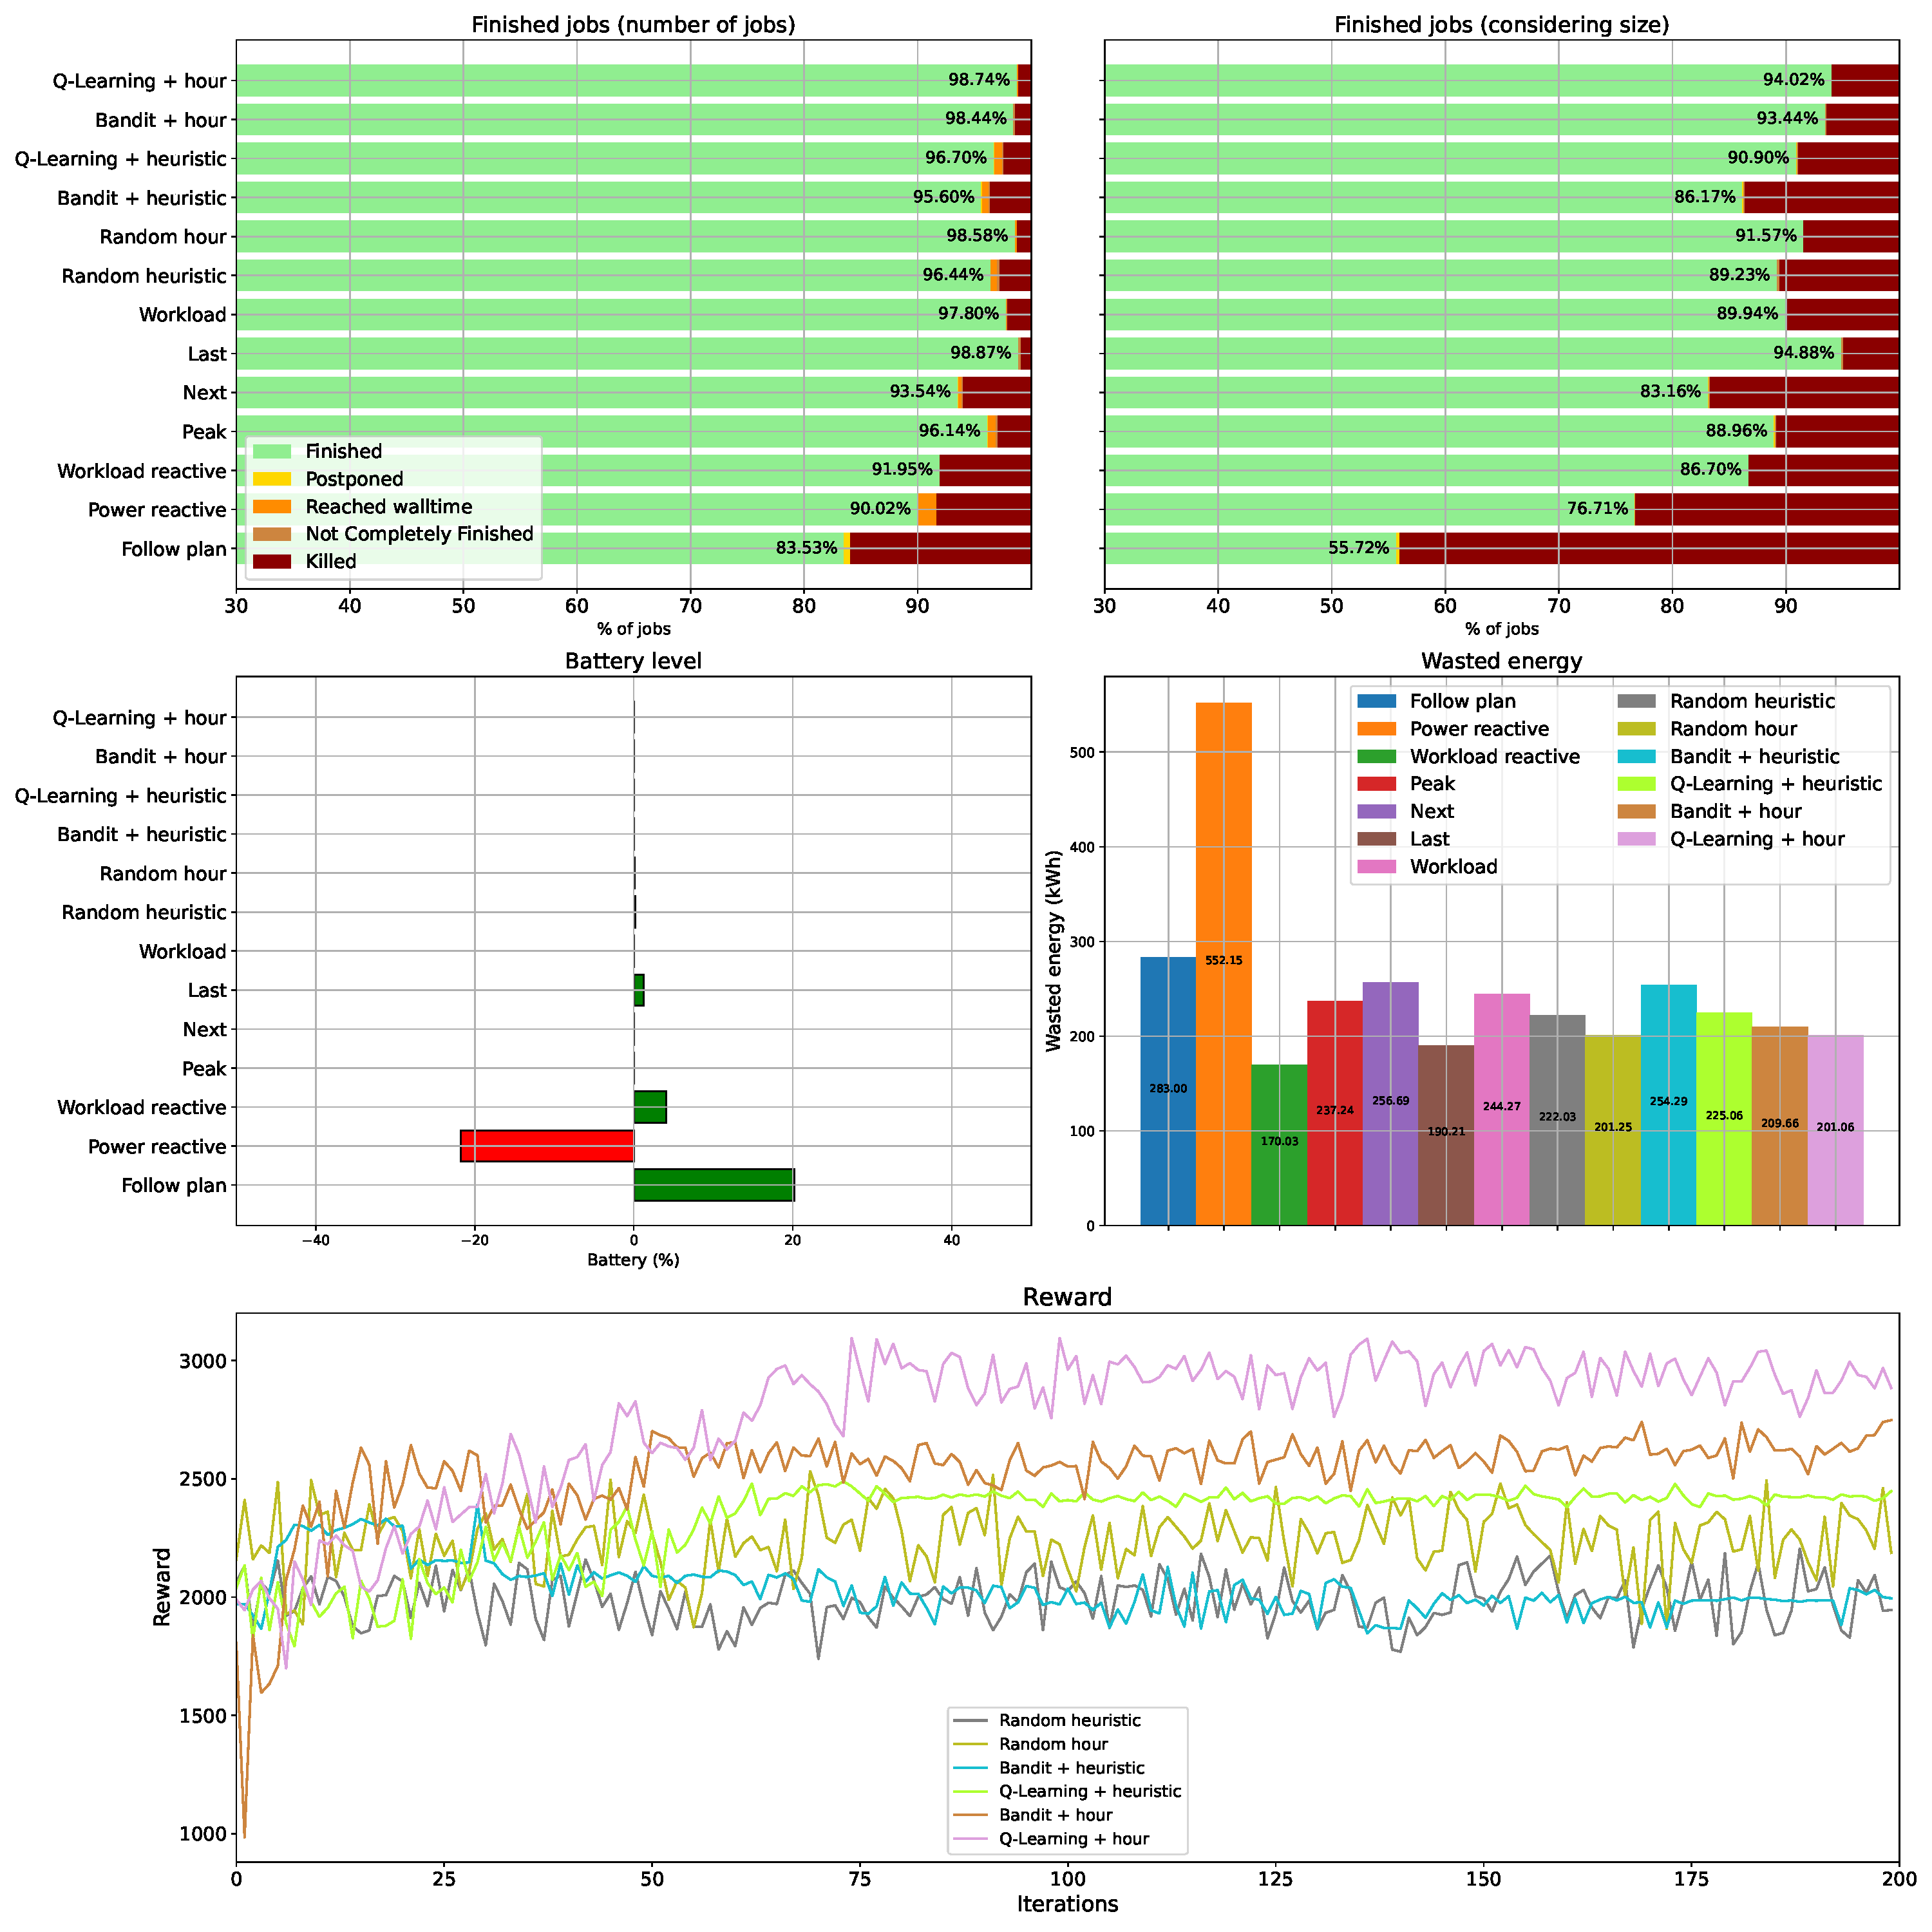
\includegraphics[scale=0.29]{Images/Learning_compensations/reward_finished_spread_profile_best_workload_1_with_noise_state_delta.pdf}
%     \caption{Results of reward finished jobs spread reward in critical case 1.}
%     \label{fig:spread_reward_results_critical_1}
% \end{figure}

% \begin{figure}[!htb]
%     \centering
%     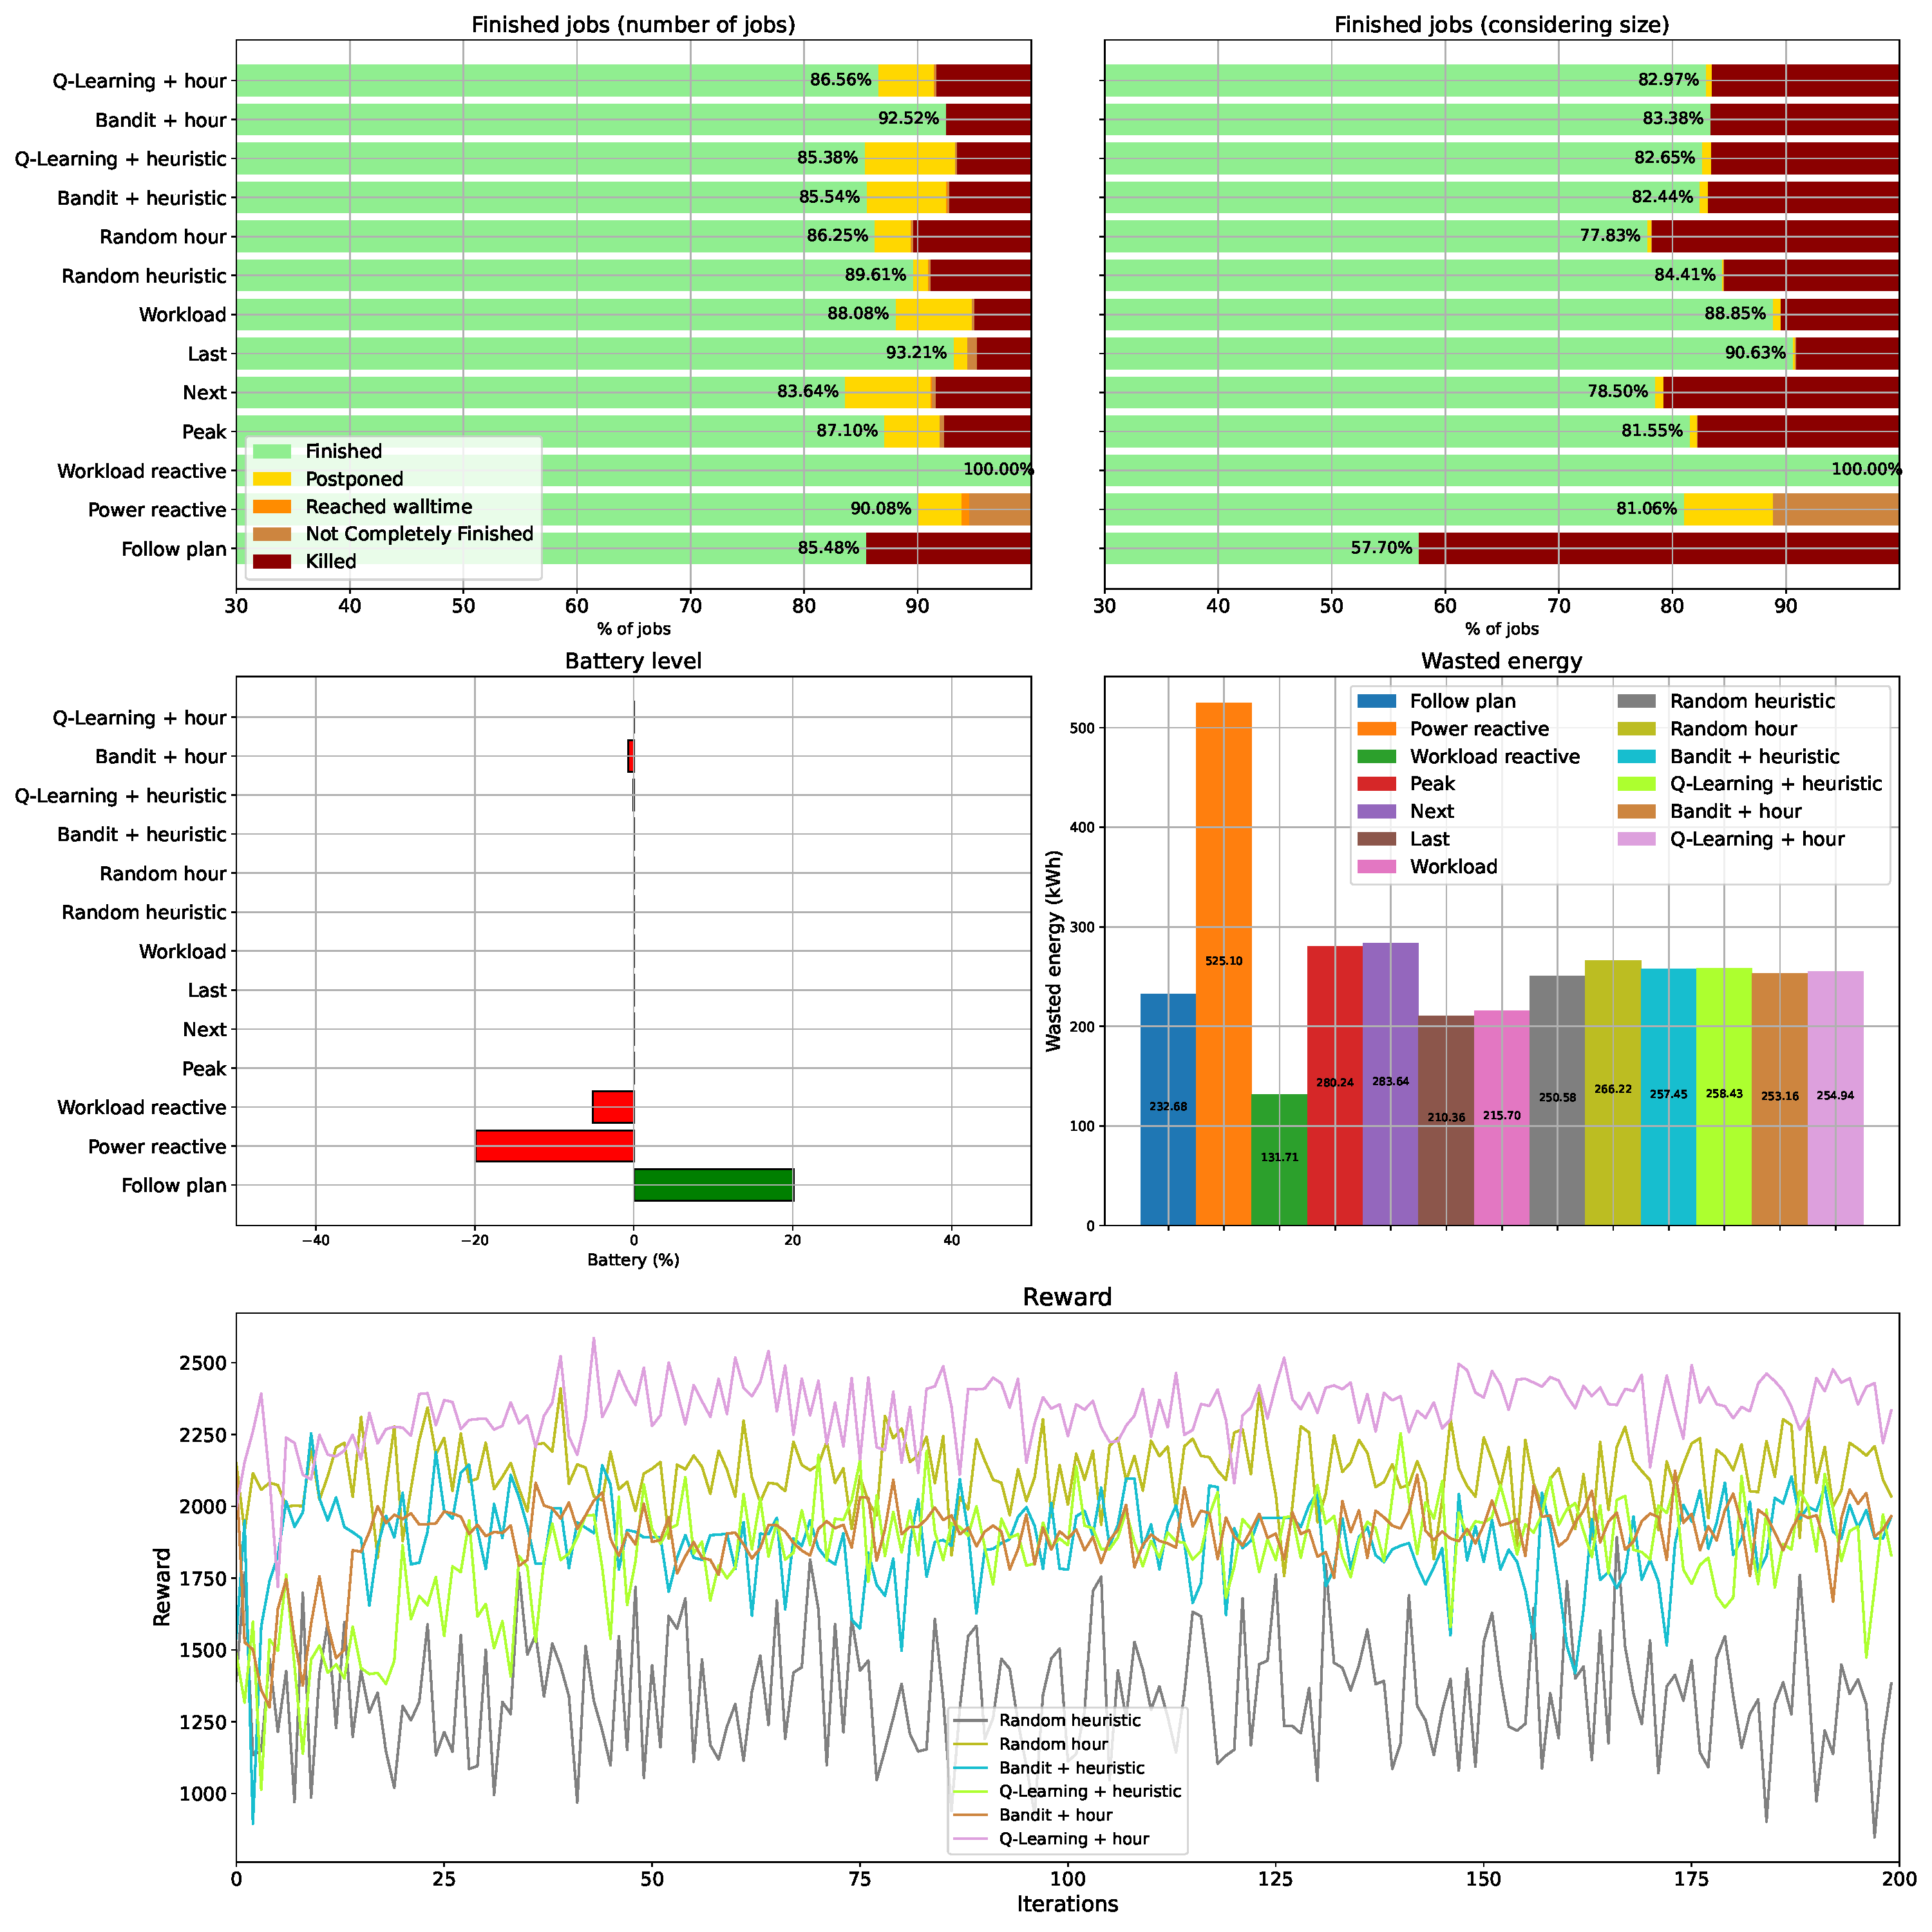
\includegraphics[scale=0.29]{Images/Learning_compensations/reward_finished_spread_profile_best_workload_2_with_noise_state_delta.pdf}
%     \caption{Results of reward finished jobs spread reward in critical case 2.}
%     \label{fig:spread_reward_results_critical_2}
% \end{figure}

% \begin{figure}[!htb]
%     \centering
%     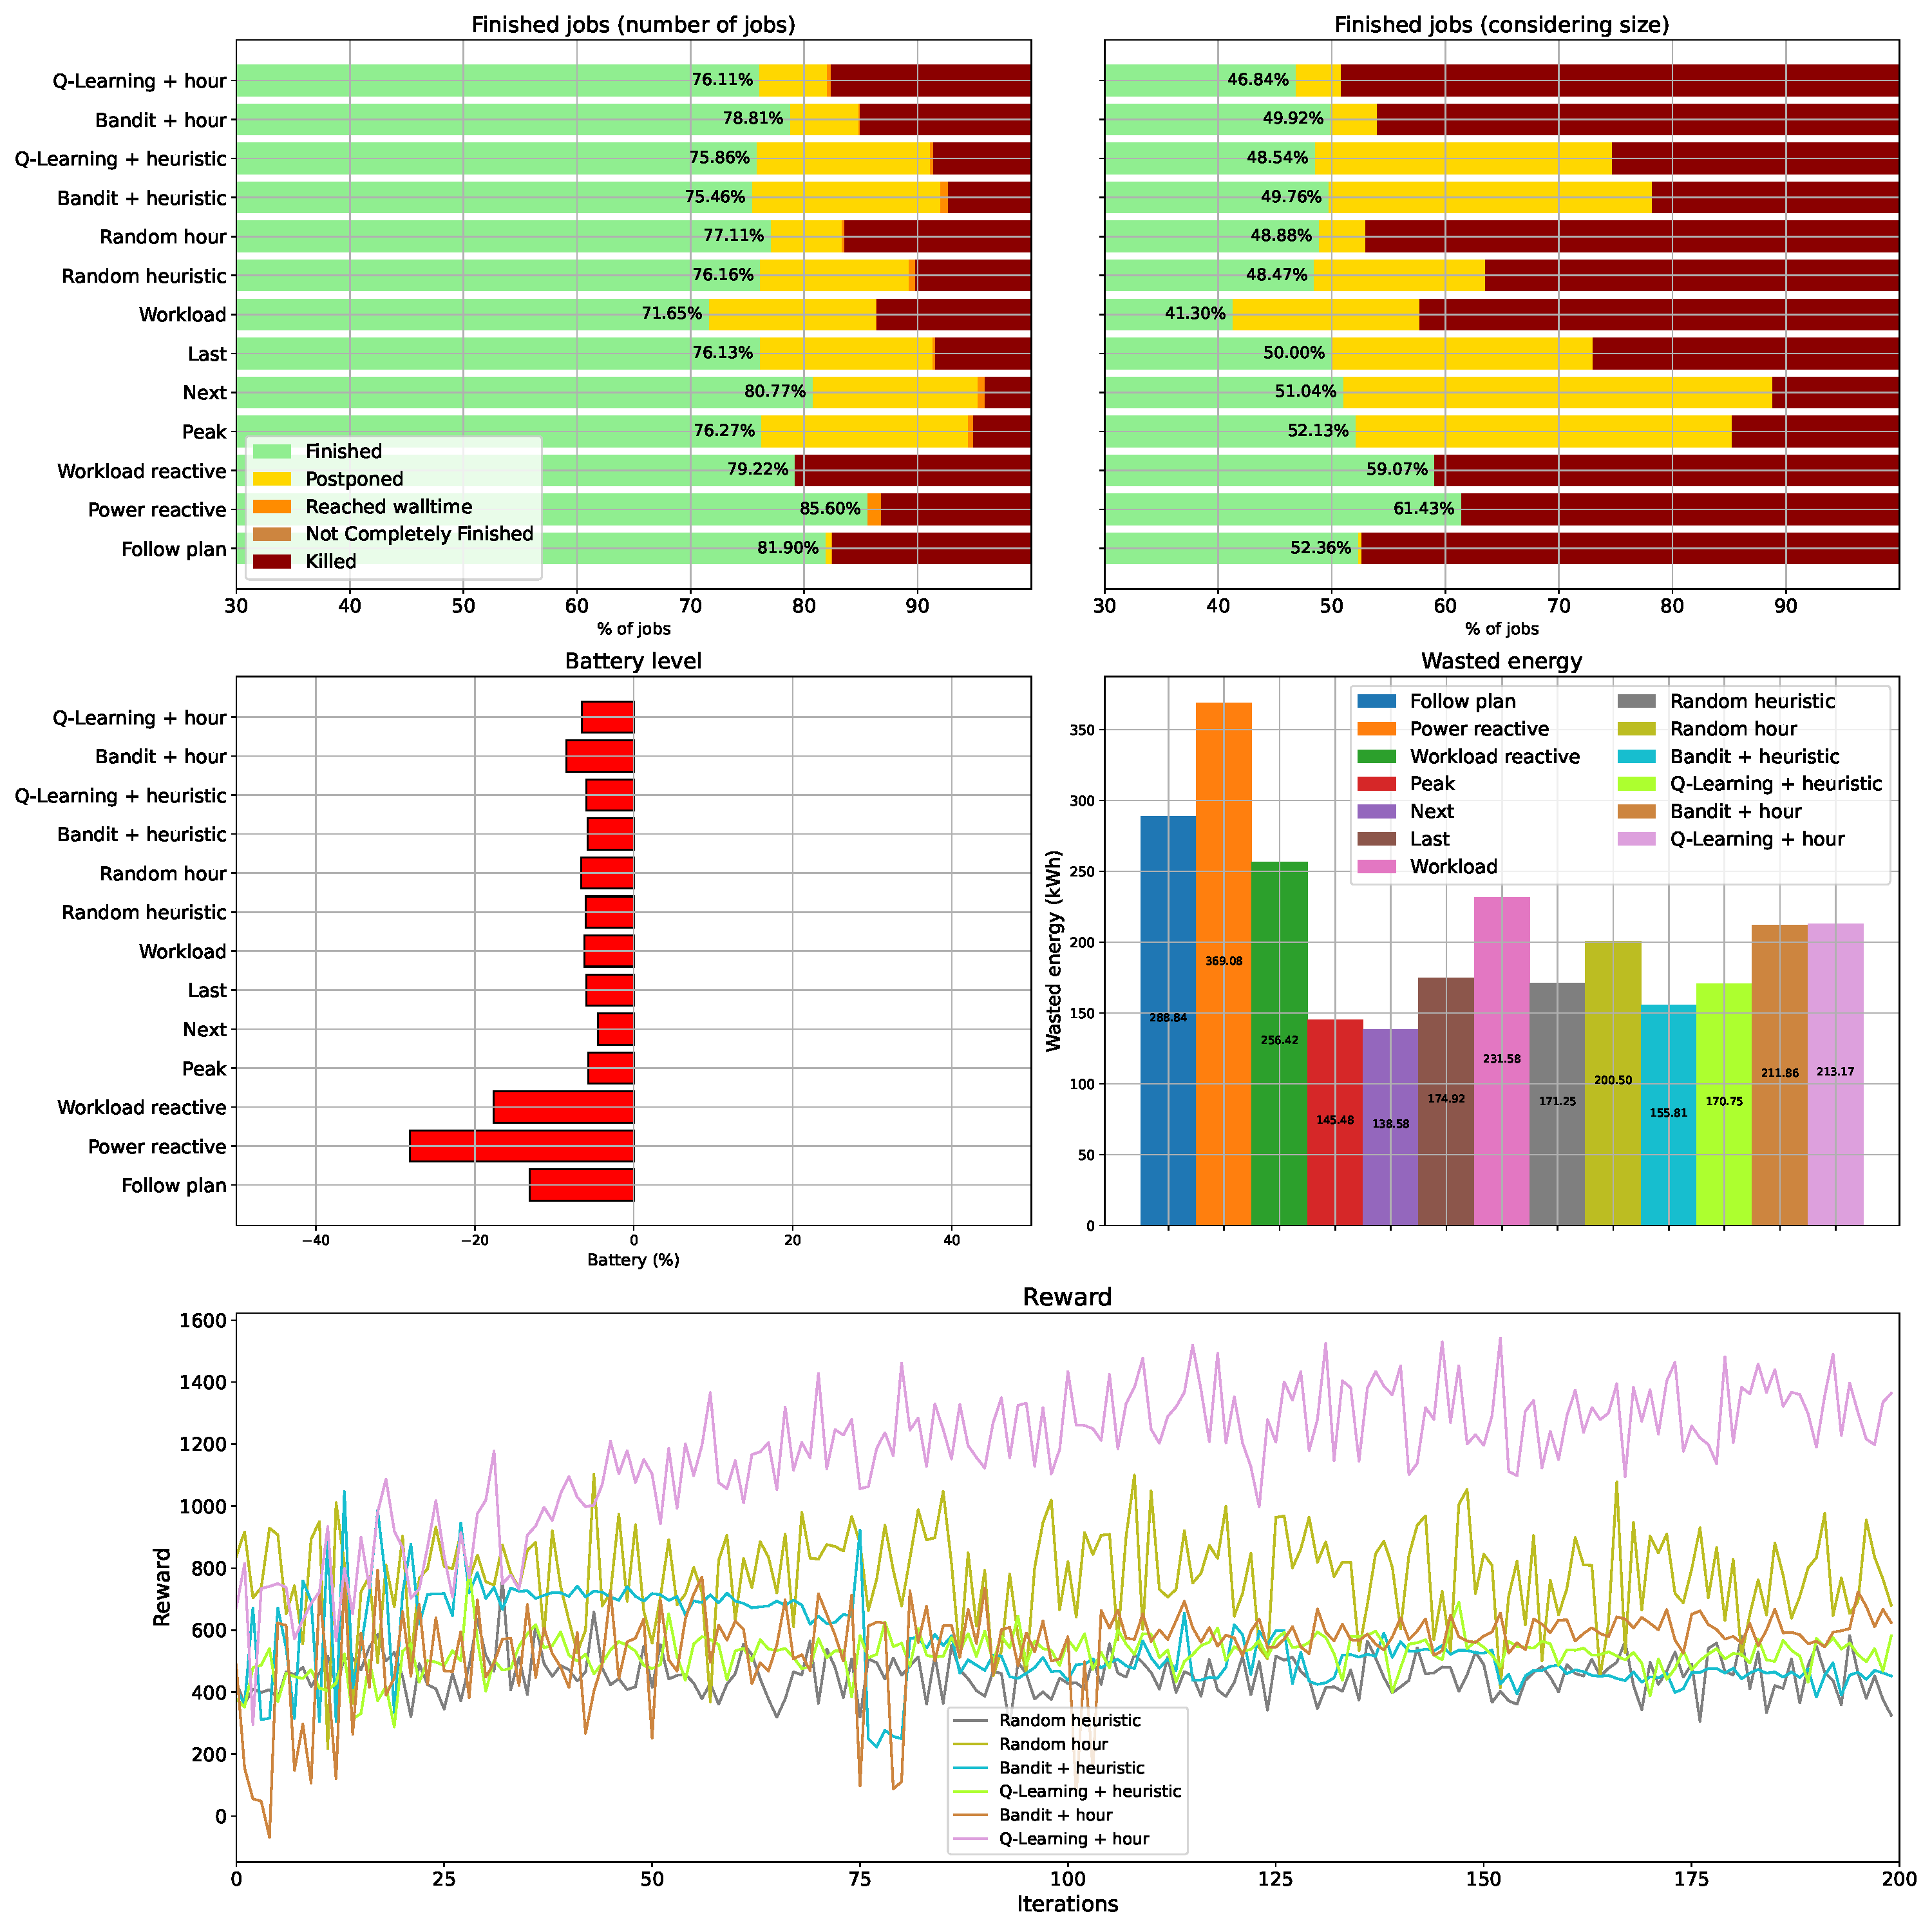
\includegraphics[scale=0.29]{Images/Learning_compensations/reward_finished_spread_profile_worst_workload_1_with_noise_state_delta.pdf}
%     \caption{Results of reward finished jobs spread reward in critical case 3.}
%     \label{fig:spread_reward_results_critical_3}
% \end{figure}

% \begin{figure}[!htb]
%     \centering
%     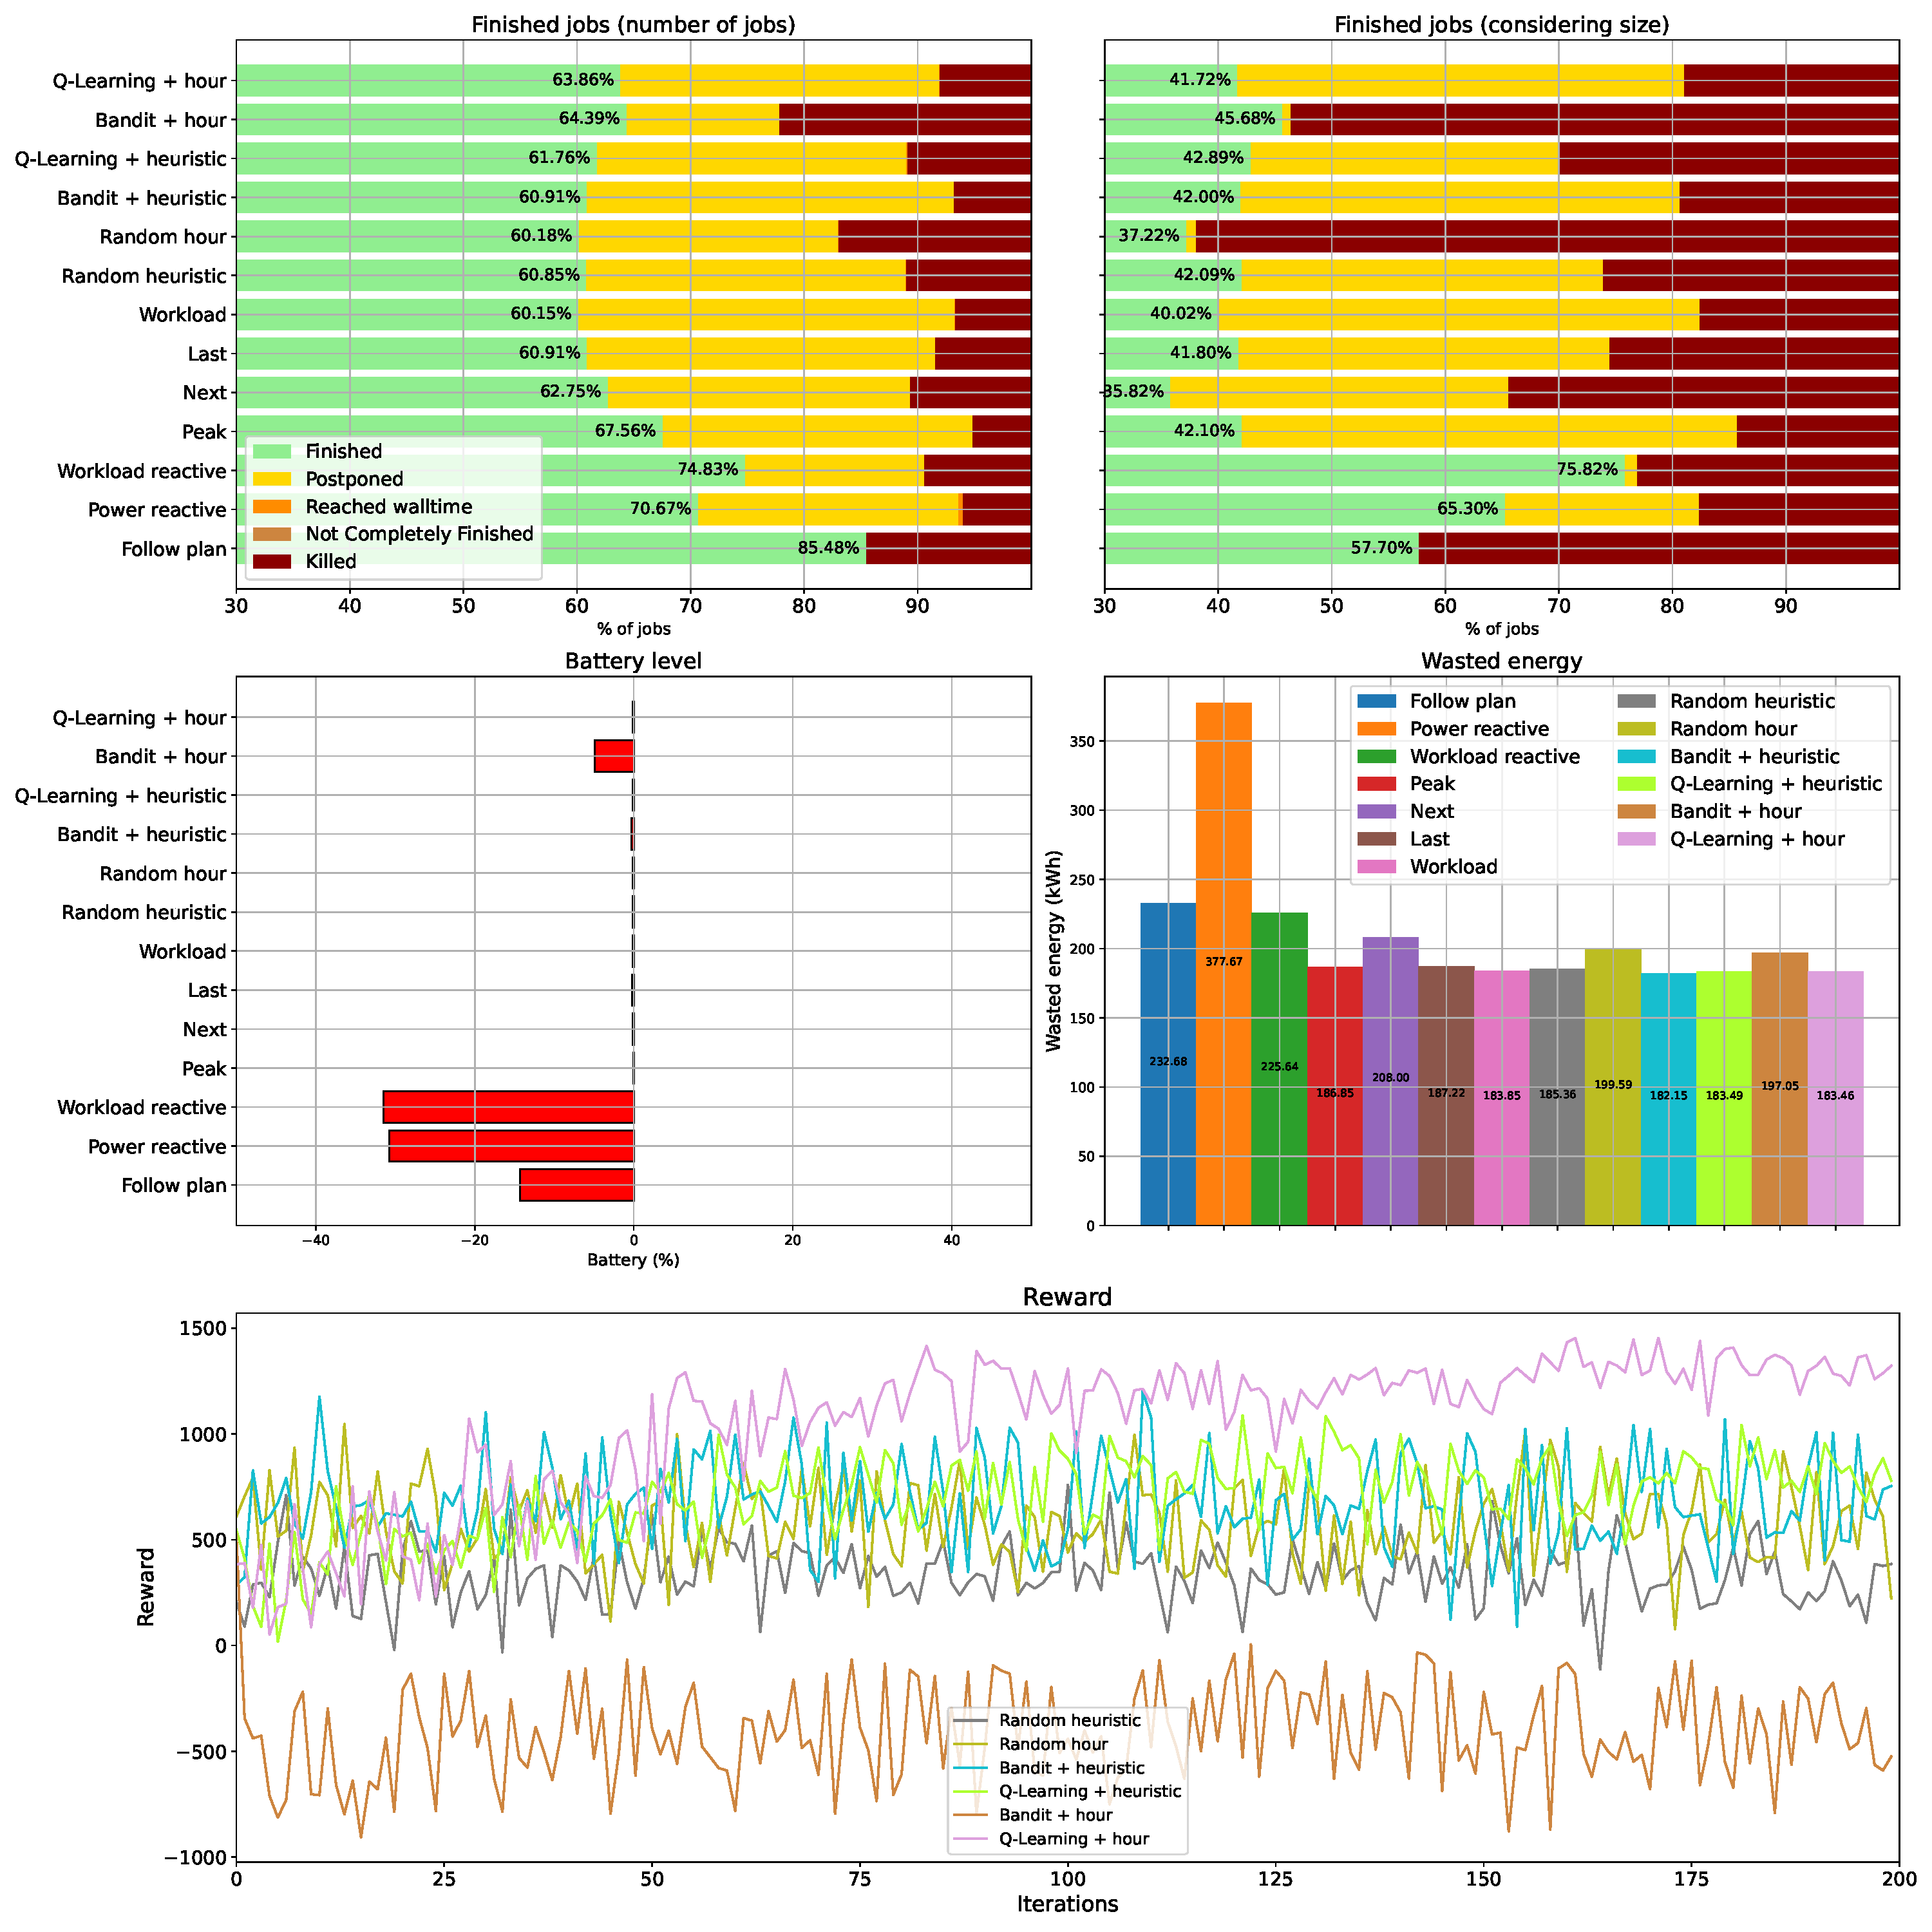
\includegraphics[scale=0.29]{Images/Learning_compensations/reward_finished_spread_profile_worst_workload_2_with_noise_state_delta.pdf}
%     \caption{Results of reward finished jobs spread reward in critical case 4.}
%     \label{fig:spread_reward_results_critical_4}
% \end{figure}

\clearpage

\subsection{Discussion}
\label{sec:learning_discussion}

After presenting and briefly discussing the results of the Reinforcement Learning algorithms in critical scenarios, this section analyzes the RL proposal deeper. We chose the critical scenarios to start with because they have more room for improvement than the random cases. The idea is that if the RL could improve in these scenarios, we could take a step further and apply RL in a scenario with more uncertainty. We proposed 200 iterations in each critical scenario, letting the RL test the different approaches to deal with them. However, even in this simplified test, our RL model was not sufficient to improve the QoS. In every case, at least one policy is better than the RL algorithms. Tables \ref{tab:ranking_started} and \ref{tab:ranking_finished} show that RL did not improve the final metrics, even after several iterations. Several reasons help to explain these results. First, we verified a difference between Bandit and Q-Learning algorithms learning. Usually, Q-Learning has a slower learning curve, going from bad rewards in the beginning but increasing over the iterations. On the other hand, Bandit does not have this learning curve. The reason is linked to the algorithm idea. While Q-Learning has a different Q-value for each state, Bandit defines a unique linear function for all states. For example, let's consider only the step variable as the state. Q-Learning can define that the best action in step 1 is \emph{Next}, in step 2 is \emph{Last}, and in step 3 is \emph{Next} again. On the other hand, Bandit defines a linear function, making it harder to do the same variation. However, while Q-Learning needs several iterations to try all action possibilities in all states, Bandit has the linear function for all states in the first iteration. Therefore, Q-Learning is slower to learn but can find the best action for each state, while Bandit is faster but must have a linear relation between state and reward. 

Our proposed RL model also introduces some problems. The three concepts (state, action, and reward) present issues. Starting with the reward, it is possible to verify in the experiments that our reward does not represent well our environment. More specifically, it rewards the decisions considering the local impact (finish more and kill less) and does not include the global QoS. This behavior introduces two problems. First, since we share the reward of finishing/killing jobs among all the steps which impacted the jobs, the RL algorithm prefers to modify steps with fewer modifications from other steps. For example, choosing \emph{Next} action would give a higher reward to the step because it receives all the reward from the step without sharing it with the other steps. The second problem is that our model only considers the jobs impacted by the actions. So, RL finds ways to impact more jobs, even with no need to receive more rewards. However, this behavior can lead to QoS degradation, such as in Figure \ref{fig:reward_from_jobs_critical_3} of \emph{Q-Learning + hour} algorithm. This algorithm increases the reward but reduces the total finished jobs. Aiming to solve this reward problem, we could change the reward model to use the global finished jobs for all actions. Nevertheless, this new reward would demand a higher learning time (more iterations) to try all combinations of actions, which can be impeditive in an online system. 

Another problem with the reward is that it is not an immediate reward. This problem means we do not know the action's reward right after applying it since it changes a future step. We discover the reward only after running the future step impacted by the compensation. Therefore, this can make it even harder to learn the best actions quickly. Besides, it is difficult to find the best share of reward for each action since several actions can impact the same future step. Regarding the action, we tested two actions: heuristic and hour. We noticed that the hour action has more freedom to choose the best action. Usually, \emph{Q-Learning + hour} is among the best results. We could not use the compensation step as action since it increases the action space, demanding higher learning time (more iterations). Future work can introduce a more flexible action space. 

Finally, the last problem of our model is the state space. We defined a simplified state space to reduce the learning time. However, this state space could include some QoS metrics, such as queue length, slowdown, waiting time, etc. Another big problem that the state could solve is related to the SoC. As mentioned before, the scheduler kills the jobs when the SoC arrives at $SoC_{min}$. So, it chooses future steps without knowing the impact of the action on the SoC. It would be interesting to introduce the expected SoC time series in the state. However, time series has too much information for the RL state, demanding a migration to a more complex algorithm, such as Deep Reinforcement Learning. This algorithm introduces a neural network to find the relation between a complex state to the expected reward. However, this kind of algorithm demands more learning time and more computational effort to maintain. Since it is heavier than a simple RL, this kind of algorithm also expends more energy, which is the opposite of what we look for. 

Regarding the impact of the moment of job arrival and having more or less energy, we could see that critical case 1 with more energy and jobs in the beginning was the best result of RL (see Figures \ref{fig:started_reward_results_critical_1} and \ref{fig:touched_reward_results_critical_1}), being close to the best algorithm (\emph{Last} policy). However, this case is the simplest one, with even \emph{Random Step} having good results. The other results show that even with several repetitions (iterations), RL could not learn the best moment to place the compensations. For example, in critical case 2, we expected the RL to have similar results to the \emph{Last} policy since the jobs arrived in the end. However, this was not the case. The cases with less energy were even worse, having distant results from the best policies.

Another problem that could be solved by changing the learning algorithm is decision dependency. Decision dependency means that the actions are chained. So, the best actions in the last steps depend on the first steps actions. These chained decisions, linked to the global reward, turn this problem really hard to solve using a simple RL algorithm. Additionally, we still maintain scheduling and compensation divided. So, the scheduling can start new jobs even if the SoC is in a dangerous place or if the battery does not have the energy to maintain this job running until the end. A new algorithm should mix compensations and scheduling decisions, improving the decisions. Due to the complexity of all these elements, our next approach will be a new heuristic that mixes all these aspects. Chapter \ref{cha:heuristic} presents this heuristic.

\section{Conclusion}
This chapter presented a new model for solving the compensation problem using Reinforcement Learning algorithms. We presented two algorithms: Bandit and Q-Learning. The algorithms analyze the state, trying to find the best compensation steps. We proposed two rewards linked to QoS. Then, we presented the results and a discussion. The results show that our problem could not be solved by a simple RL algorithm due to the different constraints. Therefore, the next chapter presents a new heuristic, which mixes compensations and scheduling decisions.